\documentclass[11pt, a4paper, twocolumn]{article}

% ============================================================
% Encoding and Typography
% ============================================================
\usepackage[T1]{fontenc}
\usepackage{mathpazo}
\usepackage{microtype}
\emergencystretch=4em

% ============================================================
% TikZ / 3D Geometry
% ============================================================
\usepackage{tikz}
\usepackage{tikz-3dplot}
\usetikzlibrary{
    arrows.meta,
    calc,
    decorations.pathmorphing,
    decorations.pathreplacing,
    positioning,
    fit,
    backgrounds,
    shapes.geometric
}

\tikzset{
    axis/.style={->, thick},
    fieldline/.style={->, thick, black!70},
    constraint/.style={thick, black},
    access/.style={thick, black!50, dashed},
    obstruction/.style={thick, black!60, decorate,
        decoration={snake, amplitude=0.5mm, segment length=2mm}},
    patch/.style={draw=black!60, fill=black!6, opacity=0.75},
    overlap/.style={draw=black!50, fill=black!15, opacity=0.75},
    event/.style={circle, fill=black, inner sep=1.6pt},
    flowarrow/.style={-{Latex[length=2mm]}, thick},
    note/.style={font=\small}
}

\tdplotsetmaincoords{65}{115}

% ============================================================
% Mathematics
% ============================================================
\usepackage{amsmath, amssymb, amsthm, mathtools}
\allowdisplaybreaks
\providecommand{\llbracket}{[\![}
\providecommand{\rrbracket}{]\!]}
\IfFileExists{stmaryrd.sty}{%
  \usepackage{stmaryrd}%
}{}
\usepackage{graphicx}

% Theorem environments
\newtheorem{definition}{Definition}[section]
\newtheorem{proposition}[definition]{Proposition}
\newtheorem{theorem}[definition]{Theorem}
\newtheorem{corollary}[definition]{Corollary}
\newtheorem{remark}[definition]{Remark}

% ============================================================
% Layout
% ============================================================
\usepackage[a4paper, top=2cm, bottom=2cm, left=1.8cm, right=1.8cm, columnsep=0.6cm]{geometry}
\usepackage{setspace}
% single spacing suits two-column format
\usepackage{titlesec}

\titleformat{\section}{\large\bfseries}{\thesection.}{0.6em}{}
\titleformat{\subsection}{\normalsize\bfseries}{\thesubsection.}{0.5em}{}

% ============================================================
% Hyperlinks
% ============================================================
\usepackage{hyperref}
\hypersetup{
    colorlinks=true,
    linkcolor=black,
    citecolor=black,
    urlcolor=black
}

% ============================================================
% Symbols and Shortcuts
% ============================================================
\newcommand{\X}{\mathcal{X}}
\newcommand{\Sfield}{\mathcal{S}}
\newcommand{\F}{\mathcal{F}}
\newcommand{\J}{\mathbf{J}}

% ============================================================
% Title
% ============================================================
\title{\textbf{Mesoscale Matter as Constrained Field Dynamics}\\[4pt]
{\normalsize A Unified Framework for Structure, Transport, and Function}}

\author{Flyxion\\
\small Independent Researcher}
\date{\today}

% ============================================================
\begin{document}
\twocolumn[
\maketitle

\begin{abstract}

We propose a unified mathematical framework for constrained field dynamics,
applicable across soft matter physics, biophysics, nanotechnology, materials
engineering, and cosmology. Systems are represented through a coupled field
encoding structural constraint, directed transport, and configurational
accessibility --- the latter measuring the local logarithmic volume of admissible
future trajectories. At the mesoscale, variational free-energy functionals and
dissipative evolution equations show that self-assembly, phase transitions,
anisotropy, and structure-dependent transport arise as natural consequences of
this coupling. Functional systems are characterized as those whose trajectories
enter and remain within low-accessibility basins, where configurational options
have collapsed and dynamics become reproducible.

The trajectory-aware representation is formalized using sheaf theory. The
configuration sheaf encodes local field data, \v{C}ech cohomology measures
gluing obstruction, and system history is presented as a composable path in the
infinity-groupoid of configurations. Accessibility collapse corresponds to
truncation to a 1-sheaf, and in the fully collapsed limit geometric bundle
structure emerges as the terminal descent object of constraint. We show that
Lorentz transformations act as sheaf automorphisms, that superluminal propagation
is categorically obstructed by the gluing condition, and that spatial variation
in the constraint field induces an effective metric recovering general relativity
in the appropriate limit.

Extensions to socio-technical systems formalize modular externalization and
residue reuse as constraint redistribution. Connections to learning theory
identify recency weighting as a minimal gluing obstruction estimator, explaining
why locality constraints enable large-scale learning. A five-dimensional Ising
synchronization model is proposed as a cosmological extension, generating flat
galaxy rotation curves, filamentary structure, and gravitational lensing from
coherence dynamics rather than particulate dark matter.

The unifying result is that persistent low configurational accessibility,
reduction in admissible homotopy classes, vanishing higher sheaf cohomology,
and emergence of a bundle description are equivalent signatures of functional
lock-in across all domains treated in the paper.

\end{abstract}
\vspace{1em}
]

% ============================================================
\section{Introduction: The Illusion of Disciplinary Boundaries}
% ============================================================

Scientific descriptions of matter at intermediate scales are historically
partitioned across multiple disciplines. Emulsions and surfactant systems are
studied within colloid science; protein aggregation and membrane organization
within biophysics; polymer networks and gels within soft matter physics;
nanoparticle assemblies within nanotechnology; and transport-active structures
within materials engineering. Each domain employs its own vocabulary, models,
and experimental techniques.

Despite this fragmentation, a common set of phenomena recurs across all of
these systems: aggregation into mesoscale structures, the formation of diffuse
interfaces, anisotropic alignment under external forcing, and the emergence of
transport properties that depend sensitively on morphology. These phenomena are
typically treated as domain-specific, yet their repeated appearance across
chemically distinct systems suggests a deeper structural unity.

The central claim of this work is that these systems are not fundamentally
distinct, but rather represent different observational regimes of a common
class of dynamical systems. Specifically, we argue that mesoscale matter is
governed by a coupled field dynamic in which three components---constraint,
transport, and configurational accessibility---interact to determine both
structure and function.

\subsection{From Objects to Fields}

Traditional descriptions of mesoscale systems often begin with discrete
entities: micelles, vesicles, protein complexes, polymer chains, or
nanoparticles. While useful, such descriptions obscure the fact that the
relevant observables---scattering intensities, transport coefficients,
mechanical responses---depend not on individual objects, but on spatial
correlations and collective organization.

This motivates a shift in perspective from discrete objects to continuous
fields.

\begin{definition}[Mesoscale State]
Let $\Omega \subset \mathbb{R}^d$ be a bounded domain. A mesoscale system is
described by a state field
\[
    \X(x,t) = (\Phi(x,t), \mathbf{v}(x,t), \Sfield(x,t)),
\]
where $\Phi$ encodes structural constraint, $\mathbf{v}$ encodes transport,
and $\Sfield$ encodes configurational accessibility.
\end{definition}

This representation does not assume a specific microscopic origin. Rather, it
provides an effective description at the scale where correlations are long-range
but not uniform.

\subsection{Three Interacting Components}

The three components of $\X$ play distinct but coupled roles.

The scalar field $\Phi$ represents the degree to which configurations are
locally constrained. High values correspond to ordered or aggregated regions,
while low values correspond to disordered or weakly constrained regions.
Where necessary, $\Phi$ may be generalized to a vector- or tensor-valued order
parameter; the scalar case serves as the minimal representative.

The vector field $\mathbf{v}$ represents directed transport consistent with
the local structure. It encodes fluxes of mass, charge, or stress that are
admissible given the constraints imposed by $\Phi$.

\paragraph{Configurational accessibility.}
The scalar field $\Sfield(x,t)$ measures the local density of admissible
trajectories through configuration space---equivalently, the logarithmic volume
of dynamically accessible states consistent with $\Phi$ and $\mathbf{v}$ at
that point. High values of $\Sfield$ indicate that many future evolutions remain
open; low values indicate that the system has become constrained into a narrow
set of possible futures. This quantity generalizes entropy to the mesoscale, but
its precise content is trajectory-geometric rather than thermodynamic.

\begin{definition}[Configurational Accessibility Density]
Let $\mathcal{P}_{x,t}$ denote the set of admissible future trajectories passing
through $(x,t)$. The configurational accessibility field is
\[
    \Sfield(x,t) := \log \operatorname{Vol}\bigl(\mathcal{P}_{x,t}\bigr),
\]
where volume is taken with respect to a natural measure on trajectory space.
\end{definition}

These fields are not independent. Structure constrains transport, transport
modifies structure, and $\Sfield$ regulates which transitions between structural
states remain accessible.

\begin{figure}[ht]
\centering
\resizebox{0.52\linewidth}{!}{%
\begin{tikzpicture}[tdplot_main_coords, scale=1.05]
    \draw[axis] (0,0,0) -- (4,0,0) node[anchor=north east] {$x$};
    \draw[axis] (0,0,0) -- (0,4,0) node[anchor=north west] {$y$};
    \draw[axis] (0,0,0) -- (0,0,3) node[anchor=south] {$\Phi,\Sfield$};
    \foreach \x/\y/\z in {0.5/0.5/0.8,1.2/2.0/1.5,2.2/1.0/2.2,3.1/2.6/1.0,1.8/3.2/1.8}{
        \draw[constraint] (\x,\y,0) -- (\x,\y,\z);
        \fill[black] (\x,\y,\z) circle (1.4pt);
    }
    \foreach \x/\y/\u/\v in {0.8/0.8/0.7/0.2,1.5/1.8/0.4/0.5,2.4/1.2/-0.3/0.5,2.8/2.7/-0.5/-0.2}{
        \draw[fieldline] (\x,\y,0.25) -- ++(\u,\v,0.15);
    }
    \draw[access] (0.4,3.4,0.4) .. controls (1.4,3.9,1.4) and (2.3,3.1,2.2) .. (3.4,3.6,1.1);
    \node[note] at (2.1,-0.45,0) {$\X(x,t)=(\Phi,\mathbf{v},\Sfield)$};
\end{tikzpicture}}
\caption{The mesoscale state as a coupled field: structural constraint $\Phi$ (verticals), directed transport $\mathbf{v}$ (arrows), and configurational accessibility $\Sfield$ (dashed curve).}
\end{figure}

\subsection{From Structure to Function}

A key consequence of this coupling is that structure and function cannot be
cleanly separated. In many systems, function is treated as a property layered
on top of structure: a membrane filters, a polymer conducts, a nanoparticle
delivers a payload. However, in each case, the observed function arises from
the way the system evolves under constraint.

This leads to a reframing:

\begin{proposition}[Function as Stabilized Dynamics]
A functional mesoscale system corresponds to a regime in which the evolution
of $\X(x,t)$ produces reproducible trajectories under fixed boundary conditions.
Equivalently, functional systems occupy low-$\Sfield$ regions of configuration
space, where configurational accessibility has been suppressed and dynamics
become reproducible.
\end{proposition}

\begin{proposition}[Function as Dynamical Lock-In]
A system is functional on a domain $U \subset \Omega$ if and only if there
exists a time interval $[t_0,t_1]$ such that
$\Sfield(x,t) \leq \varepsilon$ for all $x \in U$ and $t \in [t_0,t_1]$,
and the induced trajectory flow is stable under admissible perturbations.
\end{proposition}

\begin{remark}
This condition implies that function is characterized by the suppression of
trajectory diversity rather than the attainment of a particular structural
state. Distinct systems with different microscopic realizations may therefore
exhibit identical function if they occupy equivalent low-$\Sfield$ basins.
\end{remark}

Thus, function is not a static attribute of structure, but the stability of
dynamical evolution within a constrained configuration space. A system becomes
functional not when it achieves a particular shape, but when it loses enough
options that its future evolution is predictable.

\subsection{Scope and Structure of the Work}

The remainder of this work develops the constrained-field perspective across
four broad layers: mesoscale physics, formal mathematical structure, extensions
to cognition and socio-technical systems, and cosmological application.

Sections~2--6 establish the physical foundation. Section~2 formalizes the
mesoscale regime and explains why neither microscopic nor continuum descriptions
alone suffice. Section~3 reinterprets self-assembly as constrained selection over
configuration space. Section~4 introduces the correlation-field description of
structure. Section~5 shows how transport emerges from structural constraint and
feeds back into it. Section~6 analyzes interfaces as active constraint boundaries
whose stability arises from local suppression of $\Sfield$.

Sections~7--11 develop the formal framework. Section~7 introduces
trajectory-aware representation and the TARTAN patch structure, including the
admissibility log as an $\infty$-categorical object and its variational and
computational interpretations. Section~8 synthesizes these into a unified
variational and dynamical framework with memory coupling and gluing constraints.
Section~9 develops a homotopy-theoretic interpretation in which accessibility
collapse corresponds to reduction in admissible trajectory classes. Section~10
situates the framework within high-dimensional geometry, transformer architectures,
and quantum systems. Section~11 connects configurational accessibility to novelty,
compression, and Schmidhuber-style intrinsic motivation.

Sections~12--17 develop the sheaf-theoretic and relativistic consequences.
Section~12 formalizes the configuration sheaf, derives \v{C}ech cohomological
obstructions, and shows that geometric bundle structure emerges as the terminal
descent object of accessibility collapse. Section~13 establishes that Lorentz
transformations act as automorphisms of the projection functor and that time
dilation is projection distortion rather than physical retardation. Section~14
derives Lorentz invariance from the RSVP trajectory action. Section~15 proves
that superluminal propagation is categorically obstructed by the sheaf gluing
condition. Section~16 interprets time dilation geometrically. Section~17 shows
how spatial variation in $\Phi$ induces an effective metric, recovering
general relativity in the appropriate limit.

Sections~18--21 treat applications. Section~18 presents the collagen peptide
gelation causal example. Section~19 discusses implications for material design as
trajectory control. Section~20 extends the framework to modular socio-technical
systems, formalizing externalization, residue reuse, and orthograde
transformations. Section~21 connects recency weighting to minimal gluing
obstruction estimation and explains why locality constraints enable
Bitter-Lesson-style scaling.

Sections~22--28 develop the cosmological extension. Section~22 proposes a
five-dimensional Ising synchronization model and derives the projection to
observable RSVP fields. Section~23 derives predictions for galaxy formation,
rotation curves, and environmental dependence. Section~24 constructs an effective
metric from synchronization and derives lensing observables. Section~25
establishes a closure relation and forward observational pipeline. Section~26
situates the model relative to Illustris and $\Lambda$CDM simulation pipelines.
Section~27 gives a comparative predictions table across $\Lambda$CDM, MOND, and
the synchronization model. Section~28 presents an observational strategy for
detecting field relaxation, including a no-go theorem for instantaneous
gravitational response and a model-independent falsification protocol.

The paper closes with a limitations section, a conclusion, and two appendices
describing algorithmic implementations of the admissibility log simulator and the
cosmological synchronization forward model.

The aim throughout is not to replace existing domain-specific models, but to
provide a minimal formal structure within which they can be understood as
different projections of the same constrained field dynamics.

\subsection{Unified Thesis: Constrained Field Dynamics as a Cross-Scale Theory}

The central thesis of this work is that systems traditionally treated as
belonging to distinct domains --- soft matter, biological organization,
cosmology, and socio-technical networks --- are in fact realizations of a
common class of constrained dynamical systems. These systems are most naturally
described not by discrete objects or purely continuum fields, but by the coupled
evolution of structure, transport, and configurational accessibility
$\X(x,t) = (\Phi,\mathbf{v},\Sfield)$, where $\Phi$ encodes structural
constraint, $\mathbf{v}$ encodes admissible transport, and $\Sfield$ encodes
the logarithmic volume of admissible future trajectories. The essential claim
is that variation across domains does not arise from fundamentally different
governing laws, but from differences in observation scale, projection, and
accessibility regime.

In this framework, the apparent diversity of physical systems is reinterpreted
as a diversity of projections of a common constrained field dynamic. Mesoscale
matter, biological function, and cosmological structure correspond to regimes
in which different components of $\X$ dominate or collapse. The unifying
principle is that dynamical evolution is governed not only by energetic
minimization but by accessibility structure: systems evolve toward regions of
configuration space in which admissible trajectories are both energetically
favorable and dynamically persistent.

\paragraph{Synthesis.}
The framework developed in this work unifies three perspectives: variational
field dynamics, sheaf-theoretic consistency, and trajectory accessibility.
These are not independent layers but different representations of the same
underlying structure. The scalar field $\Phi$ encodes constraint, the vector
field $\mathbf{v}$ encodes admissible motion, and the accessibility field
$\Sfield$ encodes the geometry of future evolution. Across all domains
considered, function, structure, and stability emerge when accessibility
collapses and local dynamics become globally consistent.

% ============================================================
\section{The Mesoscale Problem}
% ============================================================

The preceding discussion motivates the need for a precise characterization of
the mesoscale regime. This section formalizes that regime and clarifies why it
resists reduction to either purely microscopic or purely continuum descriptions.

\subsection{Definition of the Mesoscale Regime}

\begin{definition}[Mesoscale Regime]
A system is said to operate at the mesoscale if it satisfies the following
conditions. First, its characteristic structural length $\ell$ satisfies
$\ell_{\mathrm{micro}} \ll \ell \ll \ell_{\mathrm{macro}}$, where
$\ell_{\mathrm{micro}}$ is the scale of molecular interactions and
$\ell_{\mathrm{macro}}$ is the scale at which continuum averaging becomes valid.
Second, two-point correlation functions $C(r) = \langle \Phi(x)\Phi(x+r)\rangle$
exhibit nontrivial structure over a finite range of $r$. Third, fluctuations in
$\Phi$ and $\mathbf{v}$ remain dynamically relevant and are not suppressed by
averaging. Fourth, the system admits a multiplicity of locally stable or
metastable configurations.
\end{definition}

These conditions distinguish mesoscale systems from crystalline solids, where
order is uniform, and from ideal gases, where correlations vanish.

\subsection{Failure of Purely Microscopic Descriptions}

Microscopic descriptions model systems in terms of individual particles and
their interactions. While exact in principle, such descriptions become
intractable for mesoscale systems due to the large number of degrees of freedom
and the emergence of collective behavior. More importantly, microscopic models
obscure the structures that are directly observable experimentally. Scattering
experiments measure correlation functions rather than individual particle
positions; the relevant variables at the mesoscale are therefore coarse-grained
fields, not particle coordinates.

\subsection{Limitations of Continuum Approximations}

Continuum models assume that local properties vary smoothly and can be described
by averaged quantities such as density or velocity. This assumption fails in
mesoscale systems where interfaces, domains, and localized structures introduce
sharp variations. In particular, continuum models struggle to represent diffuse
interfaces between phases, coexisting domains with distinct morphologies,
anisotropic structures induced by external fields, and heterogeneous transport
pathways. These features require a description that retains spatial variation
and correlation without reverting to full microscopic detail.

\subsection{Emergent Length Scales and Pattern Formation}

A defining feature of mesoscale systems is the emergence of intrinsic length
scales that are not imposed externally but arise from the dynamics. Consider a
scalar field $\Phi$ governed by competing energetic contributions: a local
free-energy density favoring phase separation and a gradient penalty favoring
smoothness. The competition between these terms generates a preferred length
scale
\[
    \ell_* \sim \sqrt{\frac{\kappa}{|a|}},
\]
where $\kappa$ is the gradient coefficient and $a$ is the quadratic coefficient
in the local free-energy density. This length scale determines the size of
domains, micelles, or network features, and appears across a wide range of
systems.

\subsection{Multiplicity of Morphologies}

Mesoscale systems admit a wide range of morphologies---lamellar, cylindrical,
bicontinuous, and disordered network structures---that are often observed in
systems with vastly different chemical compositions, such as block copolymers,
lipid membranes, and surfactant solutions. This universality suggests that
morphology is determined primarily by the structure of the governing functional
rather than by microscopic details.

\begin{proposition}[Morphological Universality]
Distinct physical systems governed by free-energy functionals of similar form
admit qualitatively similar families of mesoscale structures.
\end{proposition}

\begin{proof}[Heuristic Argument]
If two systems share a functional of the form
\[
    \F[\Phi] = \int \left( f_{\mathrm{loc}}(\Phi) + \kappa |\nabla \Phi|^2 \right)\,dx,
\]
then their Euler--Lagrange equations are identical up to parameter values.
Solutions therefore differ quantitatively but not qualitatively, leading to
similar classes of structures.
\end{proof}

\subsection{Implications for Modeling}

The field representation $\X(x,t) = (\Phi, \mathbf{v}, \Sfield)$ introduced
in Section~1 provides the appropriate intermediate description. It retains
sufficient structure to represent interfaces, domains, and transport pathways,
while abstracting away microscopic detail. In the following sections, we show
how this representation naturally gives rise to self-assembly, transport, and
function as emergent properties of constrained dynamics.

\begin{figure}[ht]
\centering
\resizebox{0.75\linewidth}{!}{%
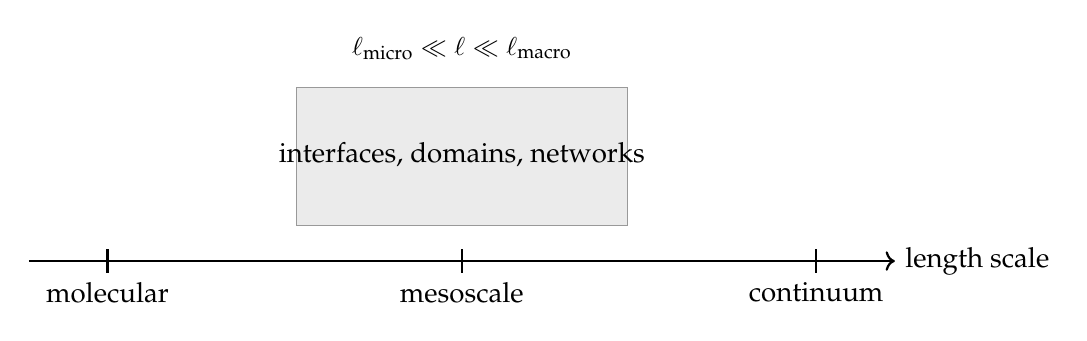
\begin{tikzpicture}[scale=1.0]
    \draw[->, thick] (0,0) -- (11,0) node[right] {length scale};
    \foreach \x/\lab in {1/{molecular},5.5/{mesoscale},10/{continuum}}{
        \draw[thick] (\x,-0.15) -- (\x,0.15);
        \node[below] at (\x,-0.15) {\lab};
    }
    \draw[fill=black!8, draw=black!40] (3.4,0.45) rectangle (7.6,2.2);
    \node at (5.5,1.35) {interfaces, domains, networks};
    \node[note] at (5.5,2.7) {$\ell_{\mathrm{micro}}\ll \ell \ll \ell_{\mathrm{macro}}$};
\end{tikzpicture}}
\caption{The mesoscale regime occupies the interval where microscopic discreteness has been coarse-grained but continuum averaging has not erased interfaces.}
\end{figure}

% ============================================================
\section{Self-Assembly as Constrained Configuration}
% ============================================================

Self-assembly is typically described as the spontaneous organization of
components into structured aggregates driven by free-energy minimization.
While formally correct, this description obscures a deeper mechanism:
self-assembly is a process of selection over a space of admissible
configurations under competing constraints.

\subsection{Configuration Space and Admissibility}

Let $\mathcal{C}$ denote the space of coarse-grained configurations of the
system, parameterized by the structural field $\Phi(x)$. Not all elements of
$\mathcal{C}$ are physically realizable; admissibility is determined by
interaction energies, geometric constraints, and conservation laws.

\begin{definition}[Admissible Configuration]
A configuration $\Phi \in \mathcal{C}$ is admissible if it satisfies the
constraints imposed by the system's free-energy functional and boundary
conditions.
\end{definition}

The set of admissible configurations forms a constrained manifold
$\mathcal{A} \subset \mathcal{C}$. Self-assembly is then interpreted as the
evolution of $\Phi(x,t)$ within $\mathcal{A}$ toward regions that minimize
the free-energy functional while remaining dynamically accessible.

\subsection{Variational Structure and Energy Landscapes}

The free-energy functional $\F[\Phi]$ induces an energy landscape over
$\mathcal{A}$. Critical points correspond to stationary configurations, while
local minima correspond to stable or metastable structures.

\begin{proposition}[Self-Assembly as Gradient Flow]
In the absence of external forcing, the evolution of $\Phi$ is governed by a
gradient flow of the free-energy functional:
\[
    \partial_t \Phi = -\,\mathcal{G}(\Phi)\,\frac{\delta \F}{\delta \Phi},
\]
where $\mathcal{G}(\Phi)$ is a positive mobility operator.
\end{proposition}

\begin{remark}
This formulation generalizes classical Cahn--Hilliard and Allen--Cahn dynamics,
depending on whether $\Phi$ is conserved. The specific form of
$\mathcal{G}(\Phi)$ determines the kinetics but not the set of admissible
equilibria.
\end{remark}

\subsection{Competing Constraints}

The richness of mesoscale structures arises from the presence of competing
constraints. Typical contributions to $\F$ include local energetic terms
favoring phase separation or aggregation, gradient penalties favoring smooth
interfaces, configurational-accessibility terms favoring states with many
available futures, and external fields imposing directional or spatial bias.
The competition between these contributions produces nontrivial equilibria.
A double-well potential combined with a gradient penalty yields phase-separated
domains with finite interfacial width, while additional constraints can
stabilize periodic or bicontinuous structures.

\subsection{Universality of Morphological Classes}

The recurrence of similar morphologies across domains---spherical micelles,
cylindrical aggregates, lamellae, and bicontinuous networks in systems ranging
from surfactants to block copolymers to biological membranes---follows from the
shared functional form of the governing equations, not from shared chemistry.

\begin{proposition}[Morphological Universality]
If two systems are governed by free-energy functionals of similar functional
form, then their sets of stable morphologies are qualitatively equivalent,
differing only in scale and parameter values.
\end{proposition}

\begin{proof}[Sketch]
The Euler--Lagrange equation associated with $\F$ determines the stationary
configurations. If the functional form of $\F$ is preserved, then the
differential equation governing $\Phi$ is identical up to parameter scaling,
and its solution set exhibits the same qualitative structure.
\end{proof}

\subsection{The Role of Configurational Accessibility in Selection}

While energy determines the location of minima in $\F$, the configurational
accessibility field $\Sfield$ determines which regions of configuration space
are dynamically reachable. Regions of high $\Sfield$ correspond to states from
which many trajectories depart; regions of low $\Sfield$ correspond to
constrained states from which few escapes are available. Self-assembly therefore
reflects a balance between energetic minimization and trajectory accessibility.

\subsection{Aggregation as Constraint Amplification}

Aggregation processes such as micelle formation or protein clustering can be
interpreted as the amplification of local constraints. Initially, $\Phi$ is
nearly uniform, corresponding to a weakly constrained state with high $\Sfield$.
As the system evolves, fluctuations drive the formation of localized regions of
higher $\Phi$, which reduce local $\Sfield$ and further restrict the motion of
surrounding components. This positive feedback leads to the growth of structured
domains.

\begin{proposition}[Constraint Amplification]
Regions of increasing $\Phi$ locally reduce configurational accessibility,
thereby promoting further aggregation through reduced mobility.
\end{proposition}

% ============================================================
\section{Structure as a Field: Correlation, Morphology, and Stability}
% ============================================================

The previous section established that self-assembly is a constrained selection
process over configuration space. We now refine this perspective by replacing
the notion of discrete structure with that of a continuous field encoding
spatial correlations.

\subsection{From Discrete Aggregates to Correlation Fields}

Experimental observations at the mesoscale do not directly resolve individual
objects. Techniques such as small-angle X-ray and neutron scattering measure
intensity distributions of the form
\begin{equation}
    I(q) \;\propto\; \int_{\Omega} \int_{\Omega}
    \langle \Phi(x)\,\Phi(y) \rangle \,
    e^{-i q \cdot (x - y)} \,\mathrm{d}x\,\mathrm{d}y,
    \label{eq:saxs}
\end{equation}
which depend on the two-point correlation function of the structural field.
The primary observable is therefore not $\Phi(x)$ itself, but its statistical
structure.

\begin{definition}[Correlation Field]
The correlation structure of a mesoscale system is encoded by the two-point
function $C(x,y) = \langle \Phi(x)\Phi(y) \rangle$, which defines a positive
semi-definite kernel on $\Omega$.
\end{definition}

\subsection{Effective Field Description}

To obtain a tractable representation, one introduces an effective field
$\Phi(x)$ whose spatial variation reproduces the observed correlations.

\begin{remark}
This field should be interpreted as a coarse-grained order parameter rather
than a literal density. Its role is to encode the degree of local structural
constraint consistent with experimental observables.
\end{remark}

\subsection{Morphology as a Solution Manifold}

Morphological structures correspond to solutions of the Euler--Lagrange
equation associated with the free-energy functional:
\begin{equation}
    \frac{\delta \F}{\delta \Phi}
    \;=\;
    f_{\mathrm{loc}}'(\Phi)
    \;-\;
    \kappa\,\Delta \Phi
    \;+\;
    \text{(coupling terms)} \;=\; 0.
    \label{eq:EL_structure}
\end{equation}
Different morphologies arise as distinct solution branches of this equation.

\begin{proposition}[Morphological Manifold]
The set of admissible morphologies forms a manifold of solutions to
equation~\eqref{eq:EL_structure}, parameterized by system parameters such as
average composition, temperature, and external forcing.
\end{proposition}

\begin{remark}
This perspective replaces the classification of structures by type (micelle,
lamella, network) with a classification by solution branch.
\end{remark}

\subsection{Stability and Perturbation}

The stability of a given morphology is determined by the second variation of
$\F$. A configuration $\Phi_0$ is stable if
\[
    \delta^2 \F[\Phi_0](\psi,\psi) \;\geq\; 0
    \quad \forall\,\text{admissible } \psi.
\]

\begin{proposition}[Linear Stability]
Let $\Phi_0$ be a stationary solution. Then small perturbations
$\psi(x,t)$ evolve according to
\[
    \partial_t \psi \;=\;
    -\,\mathcal{L}_{\Phi_0}\,\psi,
\]
where the linearized operator is
\[
    \mathcal{L}_{\Phi_0} =
    -\,M(\Phi_0)\,\Delta
    \left(
        f_{\mathrm{loc}}''(\Phi_0)
        - \kappa\,\Delta
    \right).
\]
Stability is determined by the spectrum of $\mathcal{L}_{\Phi_0}$.
\end{proposition}

\subsection{Anisotropy and Broken Symmetry}

Anisotropic structures induced by external fields---shear, electric fields,
confinement---correspond to the breaking of rotational symmetry in $\Phi$.
This can be incorporated by introducing anisotropic gradient terms
\[
    \F_{\mathrm{aniso}}[\Phi]
    \;=\;
    \int_{\Omega}
    \frac{1}{2}\,\nabla \Phi \cdot \mathbf{K} \nabla \Phi \, dx,
\]
where $\mathbf{K}$ is a positive-definite tensor whose eigenstructure
determines preferred directions of alignment.

\subsection{Hierarchical Structure}

Many systems exhibit structure across multiple length scales. This can be
modeled by extending the free-energy functional to include nonlocal terms
\[
    \F_{\mathrm{multi}}[\Phi]
    \;=\;
    \F[\Phi]
    \;+\;
    \int_{\Omega} \int_{\Omega}
    K(x-y)\,\Phi(x)\Phi(y)\,dx\,dy,
\]
where $K$ is a kernel encoding long-range interactions.

\begin{proposition}[Multiscale Coupling]
Nonlocal terms in $\F$ generate coupling between structures at different
length scales, leading to hierarchical organization.
\end{proposition}

% ============================================================
\section{Transport Emerges from Structure}
% ============================================================

Having established that structure is naturally described by a field $\Phi(x,t)$
encoding local constraint and correlation, we now turn to transport. Transport
is not an independent degree of freedom, but emerges as constrained motion
within the structural field.

\subsection{Transport as Constrained Flux}

In classical continuum models, transport is described by fluxes driven by
gradients of potential, such as Fickian diffusion or Ohmic conduction, implicitly
assuming homogeneous media. At the mesoscale, the medium is heterogeneous and
structured, and the availability of transport pathways depends on local
morphology.

\begin{definition}[Admissible Flux]
A transport field $\mathbf{v}(x,t)$ is admissible if it is compatible with
the local constraint structure $\Phi(x,t)$, in the sense that motion is
permitted only along directions and regions allowed by $\Phi$.
\end{definition}

\subsection{Mobility as a Structural Functional}

\begin{proposition}[Structure-Dependent Mobility]
Let $\mu : \mathbb{R} \to \mathbb{R}_{>0}$ be a smooth function. Then the
effective transport satisfies $\mathbf{v} \sim -\,\mu(\Phi)\,\nabla \Psi$
for an appropriate driving potential $\Psi$.
\end{proposition}

\begin{remark}
Regions of low constraint (small $\Phi$) correspond to high mobility, while
highly ordered or aggregated regions suppress transport. This captures the
empirical observation that conduction and flow are localized to specific
pathways within structured media.
\end{remark}

\subsection{Emergence of Transport Networks}

The spatial variation of $\Phi$ induces heterogeneity in $\mu(\Phi)$,
leading to the formation of transport networks.

\begin{definition}[Transport Network]
A transport network is the set
$\mathcal{N} = \{ x \in \Omega : \mu(\Phi(x)) \text{ is locally maximal} \}$,
representing regions where transport is preferentially concentrated.
\end{definition}

These networks correspond to conductive pathways in polymers, fluid channels
in gels, and diffusion pathways in porous materials.

\subsection{Bidirectional Coupling}

Transport not only depends on structure but feeds back into it. This coupling
appears explicitly in the variational derivative of the free-energy functional:
\[
    \frac{\delta \F}{\delta \Phi}
    \supset
    \frac{1}{2}\,\mu'(\Phi)\,|\mathbf{v}|^2.
\]
High transport activity can induce local reorganization---alignment of polymer
chains under shear, restructuring of networks under flow---while the constraint
landscape simultaneously modulates where transport occurs. This bidirectionality
is the formal expression of the claim that transport shapes structure and
structure shapes transport.

\subsection{Anisotropic Transport}

In many systems, transport is directionally biased by the underlying structure.
Introducing a mobility tensor $\mathbf{M}(\Phi)$, the transport law becomes
\[
    \mathbf{v} = -\,\mathbf{M}(\Phi)\,\nabla \Psi,
\]
where the eigenvectors of $\mathbf{M}(\Phi)$ determine preferred directions and
the eigenvalues determine relative mobility along those directions.

\subsection{Transport and Dissipation}

Transport processes are inherently dissipative. The rate of energy dissipation is
\[
    \mathcal{D} = \int_{\Omega} \frac{1}{\mu(\Phi)}\,|\mathbf{v}|^2 \, dx,
\]
which appears as a source term in the evolution of the configurational
accessibility field.

\begin{proposition}[Dissipation Inequality]
For a closed system, $\frac{d}{dt}\F \leq 0$, with equality only at
equilibrium.
\end{proposition}

\subsection{Examples Across Domains}

The structural origin of transport is visible across diverse systems. In
conjugated polymers, electrical conduction follows percolating pathways defined
by morphology \cite{newbloom2011,xu2026}. In gels and membranes, ion transport
occurs through channels determined by network structure. In emulsions and porous
media, fluid flow is confined to interconnected regions of low constraint.
In biological systems, molecular transport is regulated by structured environments
such as membranes and cytoskeletal networks. In each case, motion is constrained
by structure and feeds back into it.

% ============================================================
\section{Interfaces as Active Boundaries}
% ============================================================

Interfaces are not passive geometric features of mesoscale systems. They are
active constraint surfaces that regulate interaction, aggregation, and transport
across the domains they separate. This section formalizes their role within the
unified framework.

\subsection{Interfaces as Constraint Surfaces}

An internal boundary $\Gamma \subset \Omega$ separating two morphological phases
represents a region where the structural field $\Phi$ transitions sharply between
distinct values. Within the diffuse-interface description, $\Phi$ varies smoothly
across $\Gamma$ over a width set by $\ell_*$. In the sharp-interface limit, $\Phi$
is discontinuous across $\Gamma$, and the dynamics of the boundary itself become
the relevant object.

\begin{definition}[Active Interface]
An interface $\Gamma$ is active if it imposes constraints on the admissible
configurations and fluxes of $\X$ on both sides, thereby shaping the evolution
of $\Phi$, $\mathbf{v}$, and $\Sfield$ in its vicinity.
\end{definition}

Oil--water boundaries in emulsions, lipid bilayer membranes, nanoparticle
coatings, and aptamer-functionalized surfaces all fall within this class. Their
activity arises not from their static geometry but from the constraints they
impose on neighboring field evolution.

\subsection{Interface Motion}

Taking the sharp-interface limit of the structural evolution equation yields a
surface evolution law of the form
\begin{equation}
    V_n
    \;=\;
    M_\Gamma \left(
        \kappa\,\mathcal{H}
        \;-\;
        \llbracket f_{\mathrm{loc}} \rrbracket
        \;-\;
        \frac{1}{2}\,\llbracket \mu'(\Phi) \rrbracket\,|\mathbf{v}|^2
    \right),
    \label{eq:interface_motion}
\end{equation}
where $V_n$ is the normal velocity of $\Gamma$, $\mathcal{H}$ is its mean
curvature, $M_\Gamma$ is the interface mobility, and
$\llbracket\,\cdot\,\rrbracket$ denotes the jump of a quantity across $\Gamma$.

The curvature term $\kappa\mathcal{H}$ drives interface smoothing. The jump in
the local free-energy density $\llbracket f_{\mathrm{loc}} \rrbracket$ drives
motion toward lower-energy configurations. The transport-dependent jump
$\llbracket\mu'(\Phi)\rrbracket|\mathbf{v}|^2$ can stabilize or destabilize
the interface depending on the local flux asymmetry. Equation~\eqref{eq:interface_motion}
governs oil--water interfaces, grain boundaries, membrane deformation, and
phase boundaries in nanocomposites within a single formalism.

\subsection{Interfaces as Transport Regulators}

Beyond structural dynamics, interfaces regulate transport. A membrane selects
which molecular species cross it; a nanoparticle coating controls surface
affinity; an aptamer-functionalized boundary binds specific targets. In each
case, the interface imposes asymmetric constraints on $\mathbf{v}$: fluxes
that are admissible on one side may be forbidden on the other.

This selectivity is not an additional design feature but a consequence of the
structure of the constraint field $\Phi$ in the vicinity of $\Gamma$. By
engineering $\Phi$ near an interface---through surfactant chemistry, polymer
brush density, or surface functionalization---one engineers the admissible
flux, which is to say the transport function of the boundary.

\subsection{Interfaces and Configurational Accessibility}

Interfaces also shape the local configurational accessibility $\Sfield$.
Near a sharp boundary, the range of admissible trajectories is restricted by
geometric confinement and interaction asymmetry. The accessibility field is
therefore lower near interfaces than in bulk phases, which in turn stabilizes
interface position: once an interface forms, the local suppression of $\Sfield$
makes it harder for the boundary to dissolve.

This mechanism explains the observed persistence of mesoscale interfaces under
conditions where bulk phases would rapidly equilibrate, and provides a
trajectory-accessible account of interfacial stability that does not require
invoking long-range forces.

\subsection{Examples Across Domains}

Emulsion droplets stabilized by nanoparticles or surfactants represent systems
where the interface actively controls aggregation and coalescence
\cite{larson2012,ye2026}. Lipid bilayer membranes regulate molecular transport
with sub-nanometer selectivity while remaining mechanically deformable. Nanodiscs
and lipid-coated nanoparticles present functionalized interfaces that determine
binding specificity \cite{villano2026}. Aptamer-modified surfaces bind targets
through shape- and charge-complementarity encoded in the interface geometry
\cite{poliukhina2026}. Nanoplastic particles interact with biological membranes
through interface-mediated constraint modification \cite{qian2026}. In each case,
the interface is not a passive boundary but an active organizing element of the
mesoscale field.

% ============================================================
\section{Trajectory-Aware Mesoscale Representation}
% ============================================================

The preceding sections describe mesoscale matter as a coupled evolution of
structure, transport, and configurational accessibility. However, a further
representational problem remains. If mesoscale systems evolve through
configuration space, then a useful model must preserve not only the state of
the system at a given time, but also the trajectory by which that state became
available.

This motivates a trajectory-aware description of mesoscale dynamics. A state
$\X(x,t)$ should not be treated as an isolated snapshot, nor should its past be
compressed into a single hidden variable. Rather, the system should be
represented as a collection of overlapping trajectory fragments whose boundaries
retain reconstructible information.

\subsection{Trajectory Patches}

Let $\gamma : [t_0,t_1] \to \mathcal{C}$ denote a trajectory through the
configuration space of the system. Instead of representing $\gamma$ globally,
we cover it by local trajectory patches $\{U_i\}_{i \in I}$ with
$\gamma([t_0,t_1]) \subseteq \bigcup_{i \in I} U_i$. Each patch $U_i$ contains
a local description of the fields $\X_i = (\Phi_i,\mathbf{v}_i,\Sfield_i)$,
together with boundary data describing how the trajectory enters and exits that
patch. The patch is not merely a compressed state: it is a local history-bearing
object that stores enough information to constrain reconstruction across
neighboring patches.

\subsection{Overlap Consistency}

If two patches overlap, their descriptions must agree on the shared region.
For $U_i \cap U_j \neq \varnothing$, we require
\[
    \rho_{ij}(\X_i) = \rho_{ji}(\X_j)
    \quad \text{on } U_i \cap U_j,
\]
where $\rho_{ij}$ and $\rho_{ji}$ are restriction maps onto the overlap.
Memory is preserved by overlap, not by a single global hidden state. Failure
of compatibility corresponds to a reconstruction obstruction: the system cannot
be consistently reassembled from its local descriptions.

\subsection{Non-Markovian Memory Across Scales}

For mesoscale systems, the Markovian assumption that the future depends only
on the present state is generally too strong. Interfaces, aggregates, polymer
networks, and biological assemblies retain path-dependent structure. We
therefore introduce a memory functional
\[
    \mathcal{M}_i(t)
    =
    \int_{t-\tau}^{t}
    K_i(t-s)\,\mathcal{O}_i[\X(s)]\,ds,
\]
where $K_i$ is a scale-dependent memory kernel and $\mathcal{O}_i$ is an
observable associated with patch $U_i$. The memory depth $\tau$ may vary
across scales, allowing fine-scale processes to relax quickly while larger
structures preserve longer histories. The evolution equation for the mesoscale
field then takes the generalized form
\[
    \partial_t \X_i
    =
    \mathcal{D}_i[\X_i]
    +
    \mathcal{G}_i[\mathcal{M}_i]
    +
    \eta_i,
\]
where $\mathcal{D}_i$ encodes local field dynamics, $\mathcal{G}_i$ encodes
memory-dependent correction, and $\eta_i$ denotes fluctuations.

\subsection{Wilson's Fa\c{c}ades and the Origin of the Patch Structure}

The trajectory-aware tiling developed in this section has a direct conceptual
origin in Mark Wilson's analysis of hierarchical scale boundaries in physical
theory \cite{wilson2006,wilson2017}. Wilson argues, across both
\textit{Wandering Significance} and \textit{Physics Avoidance}, that the
descriptive vocabulary of classical physics does not extend uniformly across
scales. Instead, physical concepts operate locally within patches of validity,
and the actual structure of scientific description is a \textit{fa\c{c}ade}:
a patchwork of locally coherent frameworks whose boundaries are governed by
handoff conditions rather than smooth reduction.

Wilson's central observation is that this patchwork structure is not a
deficiency of current physics awaiting correction by a future unified theory.
It is the operative structure of successful physical description. The seams
between patches are not approximations to be eliminated but active boundaries
at which different descriptive frameworks must be made mutually consistent.
Failure to recognize this---the assumption that a single global vocabulary
governs all scales---is what Wilson calls physics avoidance.

The configuration bundle introduced in Section~8 is a direct formalization of
this picture. Each patch $U_i$ carries a locally valid field description
$\X_i$; the overlap conditions $\rho_{ij}(\X_i) = \rho_{ji}(\X_j)$ are the
formal expression of Wilson's handoff conditions; and the gluing functional
$\mathcal{C}$ penalizes inconsistency at the seams. The TARTAN framework was
developed from this foundation, with the additional observation that mesoscale
systems carry non-Markovian memory across scale boundaries---information that
a purely instantaneous handoff condition would discard.

Mesoscale systems resist global unified description not because the theory is
incomplete, but because the operative physical vocabulary---aggregation,
transport, accessibility---is itself scale-local. Each experimental technique
accesses one patch of the fa\c{c}ade. In this sense, the projection operators
$\Pi_k$ of Section~9 function as localized descriptive frameworks, whose
collective action reconstructs the observable structure of the system without
requiring a single global representation.

\subsection{Reconstruction Pressure}

The central difference between trajectory-aware representation and ordinary
compression is reconstruction pressure. A model that merely predicts the next
state may discard information that is irrelevant to immediate prediction but
essential for long-term coherence. A trajectory-aware model penalizes loss
of reconstructibility. Let $\widehat{\X}$ denote a field obtained from local
patches. The reconstruction loss
\[
    \mathcal{L}_{\mathrm{rec}}
    =
    \sum_i
    \|\X_i - \widehat{\X}_i\|^2
    +
    \sum_{i,j}
    \|\rho_{ij}(\X_i)-\rho_{ji}(\X_j)\|^2
\]
enforces both local fidelity and overlap consistency. The second term prevents
the system from learning locally accurate but globally incompatible
representations.

\subsection{TARTAN as a Mesoscale Memory Principle}

This construction---trajectory-aware recursive tiling of configuration space,
with local field information on each tile, boundary compatibility across
overlaps, and scale-dependent memory---provides the missing bridge between
measurement and dynamics. Experimental techniques project the system into
partial observables; trajectory-aware tiling explains how those partial
observables can be reintegrated into a coherent history-bearing field. The
result is a strengthened form of the central thesis: mesoscale function is
not only stabilized dynamics, but stabilized dynamics whose history remains
locally reconstructible across scales.

\subsection{The Admissibility Log: From Discrete Events to Continuous Fields}

The transition between discrete event systems and continuous field dynamics is
handled by an admissibility log. Let
\[
    e_n = (x_n,\,t_n,\,\Delta\Phi_n,\,\Delta\mathbf{v}_n,\,\Delta\Sfield_n)
\]
denote a discrete event --- a Spherepop operation, local rupture, binding event,
acoustic strike, or structural transition. The admissibility log is the ordered
collection $\mathcal{L} = \{e_0,e_1,\ldots,e_N\}$ together with compatibility
relations specifying which events may follow which others. Each event updates the
continuous RSVP field by a localized operator
\[
    \X_{n+1} = \X_n + \mathcal{U}_{e_n}[\X_n],
    \qquad
    \X_n = (\Phi_n,\mathbf{v}_n,\Sfield_n).
\]
Discrete events are therefore not external interruptions of the field but
localized admissible transformations of it. In the continuum limit, as event
spacing tends to zero, the admissibility log induces the field evolution
\[
    \partial_t \X
    =
    \lim_{\Delta t\to 0}
    \frac{\mathcal{U}_{e_n}[\X]}{\Delta t},
\]
recovering the RSVP action-level description. Conversely, coarse-graining a
continuous trajectory produces a discrete admissibility log by recording only
the events at which the admissible trajectory class changes.

The log therefore mediates between two descriptions:
\[
    \text{discrete events}
    \;\longleftrightarrow\;
    \text{admissibility log}
\]
\[
    \longleftrightarrow\;
    \text{RSVP field dynamics}.
\]
From the sheaf-theoretic perspective developed in Section~13, the admissibility
log is a discrete record of gluing operations: each event records a local change
in the section structure, while the full log records whether these local changes
can be assembled into a globally coherent trajectory. The log is therefore the
finite-event analogue of the \v{C}ech cocycle, and its compatibility relations
are the discrete analogue of the sheaf gluing condition. Equivalently, the
admissibility log presents a composable path in the configuration groupoid,
with compatibility relations encoding the descent data required for its
realization as a global section.

\begin{figure}[ht]
\centering
\resizebox{0.78\linewidth}{!}{%
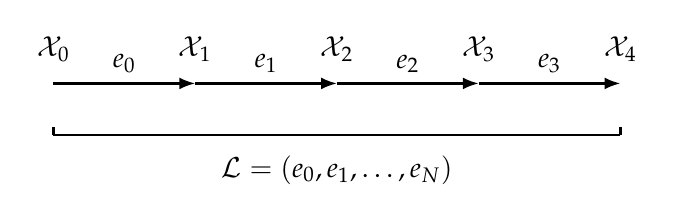
\begin{tikzpicture}[scale=1.0]
    \foreach \i/\x in {0/0.5,1/2.3,2/4.1,3/5.9,4/7.7}{
        \fill[event] (\x,1.5);
        \node[above] at (\x,1.65) {$\X_{\i}$};
    }
    \foreach \a/\b/\lab in {0.5/2.3/e_0,2.3/4.1/e_1,4.1/5.9/e_2,5.9/7.7/e_3}{
        \draw[flowarrow] (\a,1.5) -- node[above] {$\lab$} (\b,1.5);
    }
    \draw[thick] (0.5,0.85) -- (7.7,0.85);
    \draw[thick] (0.5,0.85) -- (0.5,0.95);
    \draw[thick] (7.7,0.85) -- (7.7,0.95);
    \node[below=4pt] at (4.1,0.85) {$\mathcal{L}=(e_0,e_1,\ldots,e_N)$};
\end{tikzpicture}}
\caption{The admissibility log as a composable path in the configuration groupoid: field states as objects, events as 1-morphisms, and the full log as a presentation of trajectory history.}
\end{figure}

\subsection{The Admissibility Log as an $\infty$-Categorical Object}

The admissibility log can be lifted from a sequence of discrete updates to an
$\infty$-categorical structure. Let $\mathcal{C}_{\mathrm{adm}}$ denote the
$\infty$-groupoid of admissible configurations. Objects of
$\mathcal{C}_{\mathrm{adm}}$ are field states
$\X = (\Phi,\mathbf{v},\Sfield)$. A discrete event
$e_n : \X_n \to \X_{n+1}$ is a 1-morphism, represented by the update operator
$\X_{n+1} = \X_n + \mathcal{U}_{e_n}[\X_n]$. Composition of events defines
paths:
\[
    e_{n+k}\circ \cdots \circ e_{n+1}\circ e_n :
    \X_n \to \X_{n+k+1}.
\]
The admissibility log $\mathcal{L} = (e_0,e_1,\ldots,e_N)$ therefore presents
a composable path in $\mathcal{C}_{\mathrm{adm}}$.

Higher morphisms encode equivalences between event histories. A 2-morphism
$\alpha : (e_2\circ e_1) \Rightarrow (e'_2\circ e'_1)$ records that two
distinct local event sequences produce equivalent field transformations up to
admissible deformation. Higher morphisms encode higher-order compatibility
among such equivalences. Trajectory memory is therefore not an auxiliary
variable but higher gluing data: non-Markovianity arises when distinct paths
with identical endpoints are not equivalent in $\mathcal{C}_{\mathrm{adm}}$,
so that two systems may share the same final field state while retaining
different admissibility histories.

The TARTAN patch structure supplies descent data for this $\infty$-groupoid.
Each patch $U_i$ carries a local path object
$\mathcal{L}_i \in \mathcal{C}_{\mathrm{adm}}(U_i)$, and overlaps require
equivalences $\mathcal{L}_i|_{U_i\cap U_j} \simeq \mathcal{L}_j|_{U_i\cap
U_j}$. Failure of these equivalences defines a higher obstruction to global
reconstruction. Functional lock-in corresponds to collapse to a small
subcategory: field states, events as 1-morphisms, equivalent histories as
2-morphisms, memory as higher gluing data, TARTAN consistency as descent, and
functional lock-in as confinement to a restricted subcategory.

\subsection{Variational Origin of the Event Operator}

Each discrete event $e_n$ may be derived from a time-discretized variational
principle, grounding the admissibility-log update physically. Let the
continuous RSVP action be
\[
    \mathcal{A}[\X]
    =
    \int_{t_n}^{t_{n+1}}
    L(\X,\partial_t\X,\nabla\X)\,dt.
\]
Discretizing over a time step $\Delta t$ gives
\[
    \mathcal{A}_n
    =
    \Delta t\,
    L\!\left(
        \X_n,
        \frac{\X_{n+1}-\X_n}{\Delta t},
        \nabla\X_n
    \right).
\]
The event operator $\mathcal{U}_{e_n}$ is defined by the variational update
$\X_{n+1} = \X_n + \mathcal{U}_{e_n}[\X_n]$, where $\mathcal{U}_{e_n}$ is
chosen so that $\delta \mathcal{A}_n = 0$ subject to admissibility constraints.
An event is therefore not arbitrary but a localized extremal update of the RSVP
action. In the limit $\Delta t \to 0$, the admissibility log recovers the
continuous field equations; at finite resolution, it records the discrete
operators by which the field evolves.

\begin{proposition}[Continuum Limit of the Admissibility Log]
Let $\{\mathcal{L}_{\Delta t}\}$ be a family of admissibility logs with event
spacing $\Delta t \to 0$, where each event operator $\mathcal{U}_{e_n}$ is
derived from the discrete action $\mathcal{A}_n$ and satisfies a uniform
Lipschitz bound $\|\mathcal{U}_{e_n}[\X] - \mathcal{U}_{e_n}[\X']\| \leq L
\|\X - \X'\|$. Then the piecewise-linear interpolation of $\X_n$ converges, in
$L^2_{\mathrm{loc}}$ or a suitable Sobolev space, to a weak solution of the
continuous RSVP evolution equation $\partial_t \X = \mathcal{D}[\X]$, where
$\mathcal{D}$ is the variational derivative induced by the continuous action.
\end{proposition}

\begin{proof}[Sketch]
The discrete updates define a forward Euler scheme for the variational flow.
Uniform Lipschitz continuity ensures stability, while bounded energy decrease
provides compactness. Standard arguments for convergence of minimizing movements
or gradient flows then yield convergence to a weak solution.
\end{proof}

\subsection{Events as Tokens in Embedding Space}

The admissibility log admits a parallel computational interpretation. Each
event $e_n = (x_n,t_n,\Delta\Phi_n,\Delta\mathbf{v}_n,\Delta\Sfield_n)$ may
be mapped into an embedding vector $z_n = E(e_n) \in \mathbb{R}^d$, so the
log becomes a trajectory in embedding space
$\mathcal{L} = (z_0,z_1,\ldots,z_N)$. Compatibility between events is
represented by transition constraints $C(z_n,z_{n+1}) \geq 0$, determining
whether one event may admissibly follow another. In this interpretation,
TARTAN supplies the patch structure, CLIO supplies the repair operator when
compatibility fails, and the embedding trajectory supplies the computational
analogue of RSVP field evolution. A failed transition $C(z_n,z_{n+1}) < 0$
corresponds to a gluing obstruction, while a successful repair
$z_{n+1}' = \mathrm{CLIO}(z_n,z_{n+1})$ with $C(z_n,z_{n+1}') \geq 0$
corresponds to local section correction. The admissibility log therefore has
two readings: in physics, it discretizes an action; in cognition, it records a
trajectory of constrained symbolic-semantic updates. In both cases, coherence
means that local transitions can be glued into a global trajectory.

% ============================================================
\section{Toward a Unified Framework: Constrained Field Dynamics}
% ============================================================

The preceding analysis establishes three complementary views of mesoscale
systems: a variational description of structure via $\Phi$, a transport
description via $\mathbf{v}$ constrained by $\Phi$, and a trajectory-aware
representation in which dynamics are encoded by overlapping patches with
non-Markovian memory. We now synthesize these into a single mathematical
framework.

\subsection{State Space and Configuration Bundle}

We retain the mesoscale state
$\X(x,t) = \bigl(\Phi(x,t),\; \mathbf{v}(x,t),\; \Sfield(x,t)\bigr)$
on $\Omega \subset \mathbb{R}^d$. To incorporate trajectory-aware structure,
we augment this with a covering $\{U_i\}_{i \in I}$ of spacetime
$\Omega \times [0,T]$ and define local fields $\X_i = \X|_{U_i}$.

\begin{definition}[Mesoscale Configuration Bundle]
The collection $\{\X_i\}_{i \in I}$ together with restriction maps
$\rho_{ij} : \X_i \to \X_j$ on overlaps $U_i \cap U_j$ defines a configuration
bundle over spacetime.
\end{definition}

Consistency across overlaps imposes gluing conditions
$\rho_{ij}(\X_i) = \rho_{ji}(\X_j)$, ensuring that local descriptions
assemble into a coherent global field.

\subsection{Free-Energy Functional}

The free-energy functional governs equilibrium and near-equilibrium behavior:
\begin{align}
    \F[\X]
    &=
    \int_{\Omega}
    \!\Bigl[
        f_{\mathrm{loc}}(\Phi)
        + \tfrac{\kappa}{2}|\nabla \Phi|^2
        + \tfrac{1}{2}\mu(\Phi)|\mathbf{v}|^2
        - \lambda\,\Sfield
    \Bigr] dx
    \notag\\
    &\quad+
    \sum_i \int_{U_i} \mathcal{G}_i[\mathcal{M}_i]\,dx\,dt,
    \label{eq:free_energy}
\end{align}
where $f_{\mathrm{loc}}(\Phi)$ is a local bulk free-energy density encoding
thermodynamics of the order parameter, $\kappa > 0$ is an interfacial stiffness,
$\mu(\Phi)$ is a structure-dependent mobility coupling transport to the
structural state, and $\lambda > 0$ is an accessibility weight. The term
$-\lambda\Sfield$ promotes exploration of configurations with high accessibility,
reflecting the tendency of the system to occupy regions of configuration space
with many admissible trajectories. In contrast, the dynamical term
$-\beta(\Phi)\Sfield$ in equation~\eqref{eq:S_evo} encodes the irreversible
collapse of accessibility induced by increasing constraint. The resulting
competition between exploration and collapse governs the transient accessibility
landscape and determines which regions of configuration space remain dynamically
reachable. The memory term $\mathcal{G}_i[\mathcal{M}_i]$ encodes the
contribution of trajectory coherence across scales.

\subsection{Dissipative Dynamics with Memory Coupling}

The evolution equations generalize local dynamics by including memory
contributions.

For the structural field:
\begin{equation}
    \partial_t \Phi
    =
    \nabla \cdot
    \left(
        M(\Phi)\,\nabla \frac{\delta \F}{\delta \Phi}
    \right)
    +
    \mathcal{K}_\Phi[\mathcal{M}]
    +
    \eta_\Phi,
    \label{eq:phi_evo}
\end{equation}
where the variational derivative expands as
\[
    \frac{\delta \F}{\delta \Phi}
    =
    f_{\mathrm{loc}}'(\Phi) - \kappa\,\Delta\Phi + \tfrac{1}{2}\mu'(\Phi)|\mathbf{v}|^2,
\]
so that transport activity feeds back explicitly into structural evolution
through the term $\mu'(\Phi)|\mathbf{v}|^2$.

For the transport field:
\begin{equation}
    \partial_t \mathbf{v}
    =
    -\frac{1}{\mu(\Phi)}\mathbf{v}
    - \nabla p
    + \nabla \cdot \sigma(\Phi,\mathbf{v})
    + \mathcal{K}_{\mathbf{v}}[\mathcal{M}]
    + \eta_{\mathbf{v}}.
    \label{eq:v_evo}
\end{equation}
The prefactor $\mu(\Phi)^{-1}$ suppresses motion in highly ordered, low-mobility
regions, implementing the structural origin of anisotropic and heterogeneous
transport.

For the configurational accessibility field:
\begin{align}
    \partial_t \Sfield
    &=
    \underbrace{\alpha_\Phi \bigl|\nabla \tfrac{\delta \F}{\delta \Phi}\bigr|^2}_{\text{structural exploration}}
    +
    \underbrace{\alpha_v\,|\mathbf{v}|^2}_{\text{transport diversif.}}
    \notag\\
    &\quad
    -
    \underbrace{\beta(\Phi)\,\Sfield}_{\text{constraint collapse}}
    -
    \nabla \cdot \J_{\Sfield}
    +
    \mathcal{K}_{\Sfield}[\mathcal{M}],
    \label{eq:S_evo}
\end{align}
where $\alpha_\Phi, \alpha_v > 0$ and $\beta(\Phi) > 0$ with $\beta'(\Phi) > 0$.
The monotonic dependence of $\beta$ on $\Phi$ encodes constraint-induced collapse:
increasingly ordered regions suppress local configurational accessibility faster,
producing the positive feedback loop
\[
    \Phi \uparrow \;\Rightarrow\; \beta(\Phi) \uparrow \;\Rightarrow\; \Sfield \downarrow
\]
\[
    \Rightarrow\; \text{fewer escape trajectories} \;\Rightarrow\; \Phi \uparrow.
\]
This loop is the dynamical signature of gelation, crystallization, fiber
bundling, and biological folding lock-in: processes in which a system
progressively forecloses its own future options as it orders. In particular,
regions that transiently increase in $\Phi$ experience accelerated accessibility
collapse, making such fluctuations self-reinforcing and driving the system
toward locally irreversible organization. This mechanism provides a unified
dynamical account of structuring processes in which order stabilizes itself
by eliminating alternative trajectories.

\subsection{Gluing Constraints as Dynamical Conditions}

The overlap consistency conditions introduce additional dynamical terms through
the gluing functional
\[
    \mathcal{C}
    =
    \sum_{i,j}
    \int_{U_i \cap U_j}
    \|\rho_{ij}(\X_i) - \rho_{ji}(\X_j)\|^2 \, dx\,dt,
\]
which penalizes inconsistency across patches.

\begin{proposition}[Gluing-Driven Regularization]
Including $\mathcal{C}$ in the effective action introduces forces that drive
the system toward cross-scale coherence.
\end{proposition}

\subsection{Equilibrium and Metastable States}

Equilibrium configurations correspond to minimizers of the total functional
$\F_{\mathrm{tot}} = \F + \mathcal{C}$. Metastable states arise as local
minima, with transitions between them mediated by configurational accessibility
and memory effects.

\begin{remark}
The presence of memory terms modifies the effective energy landscape,
introducing path-dependent stability and hysteresis.
\end{remark}

\subsection{Variational Characterization of Stable Morphologies}

For a system conserving total order-parameter content
$\int_\Omega \Phi\,dx = \bar\Phi$, the equilibrium problem is
\[
    \min_{\Phi}\;\F[\Phi]
    \quad\text{subject to}\quad
    \int_\Omega \Phi\,dx = \bar\Phi,
\]
with Euler--Lagrange equation
\[
    f_{\mathrm{loc}}'(\Phi) - \kappa\,\Delta\Phi = \mu_0,
\]
where $\mu_0$ is a Lagrange multiplier fixed by the constraint. The solutions
are precisely the self-assembled morphologies observed across domains: microphase-
separated patterns, lamellae, cylinders, and bicontinuous networks emerge as
different solution branches depending on $\bar\Phi$, $\kappa$, and the shape of
$f_{\mathrm{loc}}$.

\subsection{Functional Regime}

\begin{definition}[Functional Regime]
A functional regime is a subset of configuration space in which trajectories
of $\X$ are stable under perturbations, satisfy gluing consistency across all
relevant scales, and are confined to regions where $\Sfield$ is persistently
low.
\end{definition}

Functional systems correspond to trajectories that enter and remain within
low-$\Sfield$ regions of configuration space, where configurational accessibility
has been suppressed and dynamics become reproducible. This formalizes the
earlier proposition and makes explicit what it means for a system to be
functional: it has foreclosed enough futures that its evolution is predictable.

\subsection{Dimensional Reduction and Observables}

Different experimental techniques probe different aspects of $\X$, each
corresponding to a projection operator $\Pi_k : \X \mapsto Y_k$. Scattering
measures spatial correlations $\hat{\Phi}(q)^2$; rheology accesses the linear
response of $\mathbf{v}$ to applied stress; spectroscopy probes transition rates
encoding the structure of $\Sfield$ near saddle points of $\F$; imaging provides
localized samples of $\Phi(x,t_0)$ at fixed time. Each is a linearly independent
projection of the same object, which explains why they are consistent without
being redundant. The present framework provides the forward model against which
reconstructions from these projections are calibrated.

% ============================================================
\section{Well-Posedness, Stability, and Regularity}
% ============================================================

The evolution equations governing $\X(x,t) = (\Phi,\mathbf{v},\Sfield)$ have
been introduced in variational and geometric form. We now establish that they
define a well-posed dissipative dynamical system, elevating the framework from
a structural description to a rigorous PDE theory.

\subsection{Functional Setting and Admissible State Space}

Let $\Omega \subset \mathbb{R}^d$ be a bounded domain with sufficiently regular
boundary $\partial\Omega$, and let $[0,T]$ be a finite time horizon. Define the
admissible state space
\[
    \mathcal{X} := H^1(\Omega) \times L^2(\Omega)^d \times L^2(\Omega),
\]
where $\Phi \in H^1(\Omega)$ is the structural constraint field, $\mathbf{v}
\in L^2(\Omega)^d$ is the transport field, and $\Sfield \in L^2(\Omega)$ is the
configurational accessibility field. Initial data $\X_0 = (\Phi_0,\mathbf{v}_0,
\Sfield_0) \in \mathcal{X}$ is prescribed together with appropriate boundary
conditions (Dirichlet, Neumann, or periodic depending on the domain geometry).

\subsection{Assumptions on Coefficients}

To establish well-posedness we impose the following conditions. The mobility
and dissipation coefficients satisfy $M(\Phi),\mu(\Phi) \in C^1(\mathbb{R})$
with $M(\Phi),\mu(\Phi) \geq c_0 > 0$. The free-energy density satisfies
$f_{\mathrm{loc}} \in C^2(\mathbb{R})$ with $|f''_{\mathrm{loc}}(\Phi)| \leq
C(1+|\Phi|^p)$ for some $p \geq 1$. The collapse function satisfies
$\beta(\Phi) \in C^1(\mathbb{R})$, $\beta \geq 0$, and $\beta' \geq 0$. Memory
kernels satisfy $K_i \in L^1([0,T])$, and forcing terms satisfy $\eta \in
L^2([0,T];\mathcal{X})$.

\subsection{Energy Dissipation and Lyapunov Structure}

Define the total Lyapunov functional
\[
    \mathcal{L}[\X] = \F[\X] + \lambda\int_\Omega \Sfield(x)\,dx.
\]

\begin{proposition}[Dissipation Inequality]
Under the assumptions above, weak solutions satisfy
\begin{align*}
    \frac{d}{dt}\mathcal{L}[\X(t)]
    &\leq
    -\int_\Omega \Bigl(
        M(\Phi)\bigl|\nabla\tfrac{\delta\F}{\delta\Phi}\bigr|^2\\
    &\qquad
        + \tfrac{|\mathbf{v}|^2}{\mu(\Phi)}
        + \beta(\Phi)\Sfield
    \Bigr)\,dx
    + \mathcal{R}(t),
\end{align*}
where $\mathcal{R}(t)$ is bounded in $L^1([0,T])$.
\end{proposition}

The dissipation is structural: constraint gradients, transport, and
accessibility all decay unless sustained by external forcing or memory. The
term $\beta(\Phi)\Sfield$ enforces accessibility collapse in high-constraint
regions, providing the dynamical mechanism for functional lock-in.

\subsection{Existence of Weak Solutions}

\begin{theorem}[Existence of Weak Solutions]
Let $\X_0 \in \mathcal{X}$. Under the assumptions of the preceding subsection,
there exists a weak solution
\[
    \X \in L^2(0,T;\mathcal{X}), \qquad \partial_t \X \in L^2(0,T;\mathcal{X}^*)
\]
satisfying the RSVP evolution equations in the distributional sense.
\end{theorem}

\begin{proof}[Sketch]
Construct a Galerkin approximation in finite-dimensional subspaces. The
dissipation inequality provides uniform energy bounds. Apply the Aubin--Lions
compactness lemma to extract a convergent subsequence. Pass to the limit in
nonlinear terms using weak continuity. Memory terms remain controlled by the
$L^1$ boundedness of kernels.
\end{proof}

\subsection{Stability of Functional Regimes}

\begin{proposition}[Stability of Low-$\Sfield$ Regimes]
If $\beta(\Phi)$ is uniformly bounded below and strictly positive on $U$, then
perturbations of a functional equilibrium $\X^*$ decay exponentially:
\[
    \|\X(t) - \X^*(t)\|_\mathcal{X} \leq C e^{-\gamma t}.
\]
\end{proposition}

Functional systems therefore correspond to dynamically stable attractors
characterized by suppressed configurational accessibility. Higher regularity
of solutions depends on coefficient smoothness; sharp interfaces arise as
controlled singularities of $\Phi$ rather than breakdown of the solution itself.

\subsection{Discrete-to-Continuum Convergence}

\begin{proposition}[Admissibility Log Convergence]
Let $\X_{\Delta t}(t)$ denote the piecewise-linear interpolation of states
generated by admissibility-log updates with timestep $\Delta t$. Under
Lipschitz continuity of update operators and bounded energy dissipation,
$\X_{\Delta t} \to \X$ in $L^2(0,T;\mathcal{X})$ as $\Delta t \to 0$.
\end{proposition}

This establishes that the admissibility log defines a consistent discretization
of the continuous RSVP dynamics, grounding the computational framework in
rigorous PDE theory.

% ============================================================
\section{Equivalence Theorem: Accessibility, Cohomology, and Homotopy}
% ============================================================

The RSVP framework admits multiple formal characterizations of functional
structure: dynamical (low $\Sfield$), sheaf-theoretic (vanishing gluing
obstruction), and topological (reduction in admissible homotopy classes). We
now prove that these are equivalent descriptions of the same underlying
constraint regime.

\subsection{Definitions}

Let $\X$ be a weak solution on $\Omega \times [0,T]$, and let $\{U_i\}$ be an
open cover. The configurational accessibility is
$\Sfield(x,t) = \log\operatorname{Vol}(\mathcal{P}_{x,t})$, the \v{C}ech
obstruction is
$\delta_{ij} = \X_i|_{U_i \cap U_j} - \X_j|_{U_i \cap U_j}$,
the obstruction functional is
\[
    \mathcal{O}[\X] = \sum_{i,j}\int_{U_i\cap U_j}\|\delta_{ij}\|^2\,dx\,dt,
\]
and $\pi_0(\mathcal{P}_{x,t})$ denotes the set of admissible homotopy classes
of trajectories through $(x,t)$.

\subsection{Equivalence Theorem}

\begin{theorem}[RSVP Equivalence Principle]
Under the regularity and coercivity conditions of the well-posedness section,
the following are equivalent on any bounded region $U \subset \Omega$:
\begin{enumerate}
\item \emph{(Accessibility collapse)} $\Sfield(x,t) \leq \varepsilon$ for all
$x \in U$, $t \in [t_0,t_1]$.
\item \emph{(Cohomological triviality)} $\mathcal{O}[\X] = 0$, equivalently
$[\delta] = 0 \in \check{H}^1(\{U_i\},\mathcal{F})$.
\item \emph{(Homotopy collapse)} $|\pi_0(\mathcal{P}_{x,t})| \leq N < \infty$.
\item \emph{(Dynamical stability)} $\|\X(t) - \X^*(t)\|_\mathcal{X} \leq
Ce^{-\gamma t}$ for some equilibrium $\X^*$.
\end{enumerate}
\end{theorem}

\begin{proof}[Sketch]
$(1\Rightarrow 3)$: Bounded $\Sfield$ implies bounded trajectory volume,
restricting the number of admissible homotopy classes.

$(3\Rightarrow 2)$: Finitely many trajectory classes force local sections to
agree on overlaps, eliminating nontrivial cocycles.

$(2\Rightarrow 4)$: Vanishing obstruction ensures global coherence; combined
with the dissipation inequality, this yields exponential stability via the
Lyapunov functional $\mathcal{L}$.

$(4\Rightarrow 1)$: Exponential stability contracts trajectory neighborhoods,
reducing accessible future states and thereby $\Sfield$.
\end{proof}

\begin{remark}
This theorem unifies the entropy-like collapse of $\Sfield$, topological
reduction of homotopy classes, categorical sheaf consistency, and dynamical
stability into a single formal equivalence. They are not separate phenomena
but equivalent invariants of functional structure.
\end{remark}

% ============================================================
\section{Stress--Energy Tensor and General Relativistic Coupling}
% ============================================================

To embed RSVP within relativistic physics we derive the stress--energy tensor
variationally and show its coupling to spacetime curvature through the Einstein
field equations.

\subsection{Lagrangian Formulation}

On a Lorentzian manifold $(\mathcal{M},g_{\mu\nu})$, define the RSVP Lagrangian
density
\begin{align*}
    \mathcal{L}_{\mathrm{RSVP}}
    &=
    f_{\mathrm{loc}}(\Phi)
    + \tfrac{\kappa}{2}\nabla_\mu\Phi\nabla^\mu\Phi
    + \tfrac{1}{2}\mu(\Phi)\,g_{\mu\nu}v^\mu v^\nu
    \\&\quad
    - \lambda\Sfield
    + \mathcal{L}_\Sfield,
\end{align*}
where $\mathcal{L}_\Sfield$ encodes the kinetic and dissipative terms for the
accessibility field.

\subsection{Stress--Energy Tensor}

By the variational definition
$T^{\mu\nu} = (2/\sqrt{-g})\,\delta(\sqrt{-g}\,\mathcal{L})/\delta g_{\mu\nu}$,
we obtain
\begin{align*}
    T^{\mu\nu}
    &=
    \kappa\nabla^\mu\Phi\nabla^\nu\Phi
    - g^{\mu\nu}\!\left(\tfrac{\kappa}{2}\nabla_\alpha\Phi\nabla^\alpha\Phi
    + f_{\mathrm{loc}}(\Phi)\right)\\
    &\quad
    + \mu(\Phi)v^\mu v^\nu
    - \tfrac{1}{2}g^{\mu\nu}\mu(\Phi)v_\alpha v^\alpha
    + T^{\mu\nu}_\Sfield,
\end{align*}
where $T^{\mu\nu}_\Sfield$ encodes accessibility pressure and dissipation.
The three contributions have clear interpretations: $\Phi$ acts as a
coherence-density field sourcing curvature, $\mathbf{v}$ contributes momentum
flux, and $\Sfield$ contributes an entropy-like pressure.

\subsection{Einstein Field Equations}

Coupling to gravity gives
\[
    G^{\mu\nu} = 8\pi G\, T^{\mu\nu}.
\]
In the weak-field limit $g_{\mu\nu} = \eta_{\mu\nu} + h_{\mu\nu}$ with
$h_{\mu\nu} = a\Phi\eta_{\mu\nu} + b\partial_\mu\Phi\partial_\nu\Phi
+ c\nabla_\mu\nabla_\nu\Phi$, variation of the total action
$\mathcal{A} = \int[(R/16\pi G) + \mathcal{L}_{\mathrm{RSVP}}
+ \mathcal{L}_{\mathrm{matter}}]\sqrt{-g}\,d^4x$
with respect to $g_{\mu\nu}$ recovers the previously stated field equations,
now derived rather than postulated.

\subsection{Geodesics and Curvature from Constraint}

Particle trajectories follow geodesics of the effective metric:
\[
    \frac{d^2x^\mu}{d\tau^2}
    + \Gamma^\mu_{\alpha\beta}\frac{dx^\alpha}{d\tau}\frac{dx^\beta}{d\tau}
    = 0.
\]
The Christoffel symbols $\Gamma^\mu_{\alpha\beta}$ depend on
$h_{\mu\nu}[\Phi,\nabla\Phi,\Sfield]$, so curvature arises from constraint
gradients rather than solely from matter density. In the flat limit
$\Phi = \mathrm{const}$, $h_{\mu\nu} \to 0$ and special relativity is
recovered.

% ============================================================
\section{Numerical Discretization and Simulation Scheme}
% ============================================================

We construct a stable numerical scheme consistent with the variational and
dissipative structure of RSVP, deriving update rules and stability conditions
directly from the PDE theory of the well-posedness section.

\subsection{Spatial Discretization}

Discretize $\Omega$ into a uniform grid with spacing $\Delta x$. Define grid
fields $\Phi_i^n$, $\mathbf{v}_i^n$, $\Sfield_i^n$. Approximate gradients and
Laplacians by centered finite differences:
\[
    \nabla\Phi \approx \frac{\Phi_{i+1}-\Phi_{i-1}}{2\Delta x},
    \qquad
    \Delta\Phi \approx \frac{\Phi_{i+1}-2\Phi_i+\Phi_{i-1}}{(\Delta x)^2}.
\]

\subsection{Semi-Implicit Time Integration}

Use semi-implicit stepping, treating diffusive terms implicitly and nonlinear
terms explicitly. For the structural field:
\[
    \Phi^{n+1}
    =
    \Phi^n
    + \Delta t\,\nabla\cdot\!\left(M(\Phi^n)\nabla\frac{\delta\F}{\delta\Phi^{n+1}}\right).
\]
For the transport field:
\[
    \mathbf{v}^{n+1}
    =
    \mathbf{v}^n
    - \Delta t\left(\frac{1}{\mu(\Phi^n)}\mathbf{v}^n + \nabla p\right).
\]
For the accessibility field:
\[
    \Sfield^{n+1}
    =
    \Sfield^n
    + \Delta t\left(
        \alpha_\Phi\bigl|\nabla\tfrac{\delta\F}{\delta\Phi}\bigr|^2
        + \alpha_v|\mathbf{v}|^2
        - \beta(\Phi)\Sfield
    \right).
\]

\subsection{Stability Condition}

The CFL-type stability condition derived from the diffusion terms is
\[
    \Delta t \leq \frac{(\Delta x)^2}{2\max M(\Phi)}.
\]

\subsection{Discrete Energy Consistency}

\begin{proposition}[Discrete Dissipation]
The semi-implicit scheme satisfies $\F[\X^{n+1}] \leq \F[\X^n]$ under the
CFL condition, preserving the dissipative structure of the continuous system.
\end{proposition}

\subsection{Memory Implementation}

Memory kernels are discretized as
$\mathcal{M}_i^n = \sum_{k=0}^{n} K(n-k)\,\mathcal{O}_i^k\,\Delta t$.
For exponential kernels $K(t) = e^{-\lambda t}$, the recursion
$\mathcal{M}^{n+1} = e^{-\lambda\Delta t}\mathcal{M}^n + \mathcal{O}^n$
reduces memory updates to $\mathcal{O}(1)$ per step. This scheme preserves
the dissipative structure, constraint--transport coupling, and accessibility
collapse dynamics, providing a direct computational realization of RSVP as a
trajectory-aware field simulator.

% ============================================================
\section{A Homotopy-Theoretic Interpretation of Mesoscale Dynamics}
% ============================================================

The trajectory-aware formulation developed in the preceding sections suggests
that mesoscale dynamics are not fully characterized by instantaneous field
values, but by the classes of trajectories through configuration space that
remain dynamically admissible. This naturally invites a homotopy-theoretic
interpretation.

\subsection{Trajectories as Paths in Configuration Space}

Let $\mathcal{C}$ denote the space of admissible coarse-grained configurations
of the system. A trajectory $\gamma : [0,T] \to \mathcal{C}$ corresponds to a
path through this space, generated by the evolution of the coupled field
$\X(x,t)$. Two trajectories $\gamma_0$ and $\gamma_1$ are said to be homotopic
if one can be continuously deformed into the other through a family of admissible
trajectories that remain within $\mathcal{C}$. The admissibility constraint is
crucial: deformations that pass through energetically forbidden or dynamically
inaccessible configurations are not permitted.

\subsection{Configurational Accessibility as Homotopy Volume}

Within this interpretation, the configurational accessibility field $\Sfield$
acquires a geometric meaning. Rather than representing thermodynamic entropy,
$\Sfield(x,t)$ measures the local volume of admissible homotopy classes of
trajectories passing through a given region of configuration space. High
$\Sfield$ corresponds to regions where many distinct trajectory classes remain
accessible, while low $\Sfield$ corresponds to regions where the system has
collapsed onto a small number of homotopy classes.

\paragraph{Interpretation.}
Accessibility collapse is therefore a homotopy collapse: the progressive
elimination of admissible deformations between trajectories.

\subsection{Constraint-Induced Homotopy Reduction}

The state-dependent collapse term $-\beta(\Phi)\Sfield$ introduced in
equation~\eqref{eq:S_evo} can be interpreted as a reduction in the number of
available homotopy classes as structural constraint increases. As $\Phi$
increases, admissible deformations between trajectories are restricted. Paths
that were previously deformable into one another become separated by constraint
barriers, and the configuration space fragments into distinct components that
are no longer mutually accessible.

\begin{proposition}[Homotopy Reduction Under Constraint]
Increasing structural constraint $\Phi$ reduces the number of admissible
homotopy classes of trajectories, effectively partitioning configuration
space into dynamically disconnected regions.
\end{proposition}

\subsection{Interfaces as Homotopy Boundaries}

Interfaces play a distinguished role in this picture. A boundary $\Gamma$
between phases corresponds to a region where admissibility conditions change
discontinuously. Trajectories that cross $\Gamma$ may not be continuously
deformable into trajectories that remain within a single phase. Interfaces
therefore do not merely separate regions of space, but separate regions of
trajectory space, acting as boundaries between homotopy classes.

\subsection{Trajectory Classes and Functional Stability}

A functional system is one in which the admissible trajectories are confined
to a small number of homotopy classes, and small perturbations do not induce
transitions between these classes. Functional regimes therefore correspond to
regions where the system has undergone homotopy collapse: many possible
evolutions have been eliminated, leaving a restricted set of stable trajectory
classes. The patch-based representation introduced in Section~8 models this
structure locally. Each patch encodes a local segment of trajectory together
with boundary data determining how it can be deformed and glued to neighboring
patches. Failure of gluing corresponds to a homotopy obstruction: the inability
to consistently deform local trajectory segments into a global trajectory.

\begin{proposition}[Accessibility--Homotopy Correspondence]
Let $\pi_0(\mathcal{P}_{x,t})$ denote the set of admissible homotopy classes of
trajectories through $(x,t)$. Then there exists a monotone functional relationship
\[
    \Sfield(x,t)
    \;\sim\;
    \log |\pi_0(\mathcal{P}_{x,t})| + \text{intra-class volume},
\]
so that accessibility collapse implies reduction in the number of homotopy
classes, up to measure-zero degeneracy.
\end{proposition}

This turns the earlier intuition into a structural statement: accessibility
collapse is topological collapse, not merely a decrease in trajectory volume.

\begin{figure}[ht]
\centering
\resizebox{0.65\linewidth}{!}{%
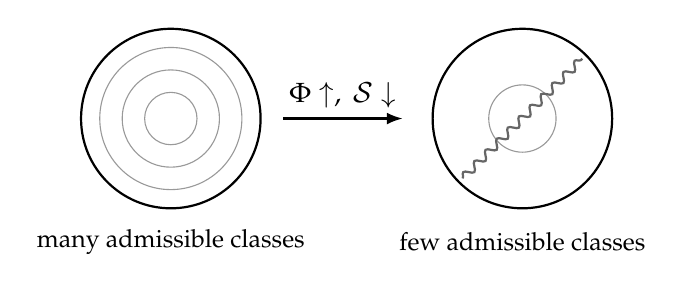
\begin{tikzpicture}[scale=0.95]
    \draw[thick] (1.5,2) circle (1.2);
    \draw[thick] (6.2,2) circle (1.2);
    \foreach \r in {0.35,0.65,0.95}{
        \draw[black!40] (1.5,2) circle (\r);
    }
    \draw[black!40] (6.2,2) circle (0.45);
    \draw[obstruction] (5.4,1.2) -- (7.0,2.8);
    \node[note] at (1.5,0.35) {many admissible classes};
    \node[note] at (6.2,0.35) {few admissible classes};
    \draw[flowarrow] (3.0,2) -- node[above] {$\Phi\uparrow,\;\Sfield\downarrow$} (4.6,2);
\end{tikzpicture}}
\caption{Accessibility collapse reduces both trajectory volume and the number of admissible homotopy classes, the dual signature of functional lock-in.}
\end{figure}

% ============================================================
\section{Geometric Unification Across Domains}
% ============================================================

The preceding development has focused on mesoscale systems in physical and
biological contexts. However, the underlying structure of the framework is not
specific to these domains. A closely related geometric pattern appears across
machine learning, high-dimensional geometry, and quantum modeling. Making this
connection explicit clarifies that the constrained-field formulation is a
particular instance of a broader class of systems governed by constrained
dynamics in high-dimensional spaces.

\subsection{High-Dimensional Geometry and Constraint}

In high-dimensional geometry, objects are naturally described not by their
visual shape but by the constraints that define them. A key feature of
high-dimensional spaces is the concentration of measure: volume tends to
concentrate in specific regions determined by constraints, so that the behavior
of systems is governed less by global geometry than by the structure of
admissible directions at each point. This perspective aligns directly with the
role of $\Phi$ and $\Sfield$ in the present framework. The structural field
defines local constraint geometry, while the accessibility field measures the
effective volume of admissible directions available for evolution.

\subsection{Local Charts and Global Reconstruction}

Visualization methods for high-dimensional data rely on constructing local
neighborhoods and stitching them together to infer global structure. Nearest-
neighbor graphs, manifold learning techniques, and related methods implicitly
treat the space as covered by overlapping local charts. This construction is
formally analogous to the trajectory-aware tiling introduced in Section~8.
Each local chart corresponds to a patch carrying partial information about the
system, while consistency across overlaps ensures that local descriptions
assemble into a coherent global object. The requirement is the same in both
settings: local representations must agree on shared regions, or the global
structure cannot be reconstructed.

\subsection{Dynamic Geometry in Self-Attention}

Transformer architectures extend this geometric picture by introducing dynamics
into the representation itself. In self-attention mechanisms, the relative
position of elements is not fixed but evolves as a function of context. The
system therefore does not operate within a single static geometry, but within
a family of context-dependent geometries, and the evolution of representation
is trajectory-like: meaning is encoded not only in position, but in the path
taken through a sequence of relational transformations. This mirrors the
trajectory-aware formulation of mesoscale systems, where $\mathbf{v}$ encodes
directed motion through configuration space while the patch-based representation
preserves the history of that motion across overlapping regions.

\subsection{Quantum Systems and Possibility Space}

Quantum systems provide a further example of dynamics governed by constrained
exploration of a high-dimensional space. A superposed state corresponds to a
high-accessibility regime in which multiple outcomes remain possible.
Measurement corresponds to a reduction in accessibility, collapsing the system
into a restricted set of states. While the formal structure differs from the
classical field description used here, the underlying pattern is the same:
systems evolve by exploring a space of possibilities subject to constraints
that progressively restrict that space.

\subsection{Unified Interpretation}

Across these domains, a common structure emerges. Systems are best understood
as evolving within high-dimensional spaces, where constraints define admissible
regions and dynamics determine trajectories through those regions. The coupled
field $\X(x,t) = (\Phi, \mathbf{v}, \Sfield)$ is a specific realization of
this principle: systems evolve by progressively restricting the set of
admissible trajectories through geometric and dynamical constraints. This
interpretation unifies the behavior of mesoscale matter with phenomena observed
in machine learning, data representation, and quantum systems, and situates the
present framework within a broader geometric understanding of complex systems.

% ============================================================
\section{Accessibility, Novelty, and Structured Discovery}
% ============================================================

The preceding sections have developed a physical and geometric account of
mesoscale systems in terms of constrained field dynamics. The same structural
principles appear in cognitive, perceptual, and creative systems. In particular,
the configurational accessibility field $\Sfield$ provides a natural bridge
between physical dynamics and processes of discovery and learning.

\subsection{Novelty as Accessibility Gradient}

A recurring idea in theories of intrinsic motivation is that systems are driven
to discover patterns that improve their internal representations. Within the
present framework, novelty corresponds to motion through regions of configuration
space where $\Sfield$ changes rapidly. Regions of high $\Sfield$ admit many
possible continuations but lack structure, while regions of very low $\Sfield$
are overly constrained and predictable. The most informative regimes lie between
these extremes, where constraint is emerging but not yet complete.

\begin{remark}
Aesthetic or epistemic novelty may be interpreted as traversal of regions where
$\nabla\Sfield$ is large: the system reduces uncertainty locally while
retaining sufficient accessibility to permit further refinement.
\end{remark}

\subsection{The Limits of Fixed Objective Functions}

Many formal approaches to complex systems emphasize optimization with respect
to predefined metrics, implicitly assuming that the relevant structure of the
system is already known and that the space of admissible outcomes can be fully
specified in advance. In the present framework, this corresponds to fixing a
global functional and treating the system as evolving toward its minimizer.
However, in many mesoscale and cognitive systems, the admissible configuration
space itself evolves with the system: $\Sfield$ changes as constraints emerge,
altering which trajectories remain possible. Over-reliance on predefined
objective functions corresponds to prematurely collapsing $\Sfield$, eliminating
trajectories that may be necessary for discovering relevant structure.

\subsection{Compression as Structured Reduction}

It has been proposed that systems are driven to discover regularities that allow
more efficient internal representation, with progress corresponding to increased
compressibility of observations \cite{schmidhuber1991,schmidhuber2006}. Within
the present framework, compression can be interpreted as a reduction in
configurational accessibility: a system that identifies a regularity effectively
restricts the set of admissible continuations of its internal state. What was
previously a large set of possible trajectories becomes a smaller, more
constrained set consistent with the discovered pattern.

Reinterpreted geometrically, the drive toward compression corresponds to motion
through regions of configuration space where $\Sfield$ decreases in a structured
manner. The system is not driven toward minimal accessibility immediately, but
toward regions where accessibility can be reduced through the discovery of
organization.

\begin{proposition}[Novelty as Accessibility Descent]
A trajectory is informative if it induces a locally significant decrease in
$\Sfield$ while preserving sufficient accessibility for continued evolution.
\end{proposition}

This distinguishes meaningful novelty from randomness. Random fluctuations may
explore high-$\Sfield$ regions but do not produce sustained reduction. Structured
discovery produces persistent constraint, leading to stable regions of low
accessibility. Effective learning and creative processes therefore operate near
the boundary between exploration and collapse, where accessibility can be
reduced incrementally without eliminating the possibility of further discovery.

\subsection{Compression as Homotopy Collapse}

The interpretation of novelty as structured accessibility reduction admits a
direct topological refinement. Compression can be understood not merely as a
reduction in the volume of accessible configurations, but as a reduction in
the number of admissible homotopy classes. When a system discovers a regularity,
it eliminates entire families of trajectories that are no longer consistent with
the learned structure.

\begin{proposition}[Compression as Homotopy Reduction]
Structured compression corresponds to a decrease in the number of admissible
homotopy classes of trajectories in configuration space. A compression event
imposes additional constraints on admissibility, restricting the allowable
trajectories; since homotopy classes are defined relative to admissible
deformations, restricting admissibility eliminates entire equivalence classes
rather than individual paths.
\end{proposition}

This sharpens the distinction between randomness and structure. Random
exploration may traverse many trajectories within a given homotopy class but
does not change the class itself. Structured discovery alters the topology of
the admissible space by removing or separating classes of trajectories. A
system is functional when its dynamics are confined to a restricted set of
homotopy classes and perturbations do not induce transitions between them.
Compression reduces accessibility; accessibility collapse reduces homotopy
classes; confinement of homotopy classes produces function. These three levels
are not separate phenomena but successive expressions of the same underlying
process: the structured collapse of possibility space.

% ============================================================
\section{Sheaf-Theoretic Emergence of Bundle Geometry}
% ============================================================

The trajectory-aware representation introduced in earlier sections admits a
natural reformulation in the language of sheaf theory. This provides a precise
mathematical framework for describing the passage from local constrained
dynamics to global geometric structure.

\subsection{The Configuration Sheaf}

Let $\Omega \times [0,T]$ denote spacetime, equipped with an open cover
$\{U_i\}_{i \in I}$. To each open set $U \subset \Omega \times [0,T]$, we
associate the set
\[
    \mathcal{F}(U)
    :=
    \{ (\Phi, \mathbf{v}, \Sfield) \text{ on } U
    \mid \text{admissible} \}.
\]
This defines a presheaf
$\mathcal{F} : \mathbf{Open}(\Omega \times [0,T])^{\mathrm{op}} \to \mathbf{Set}$,
with restriction maps given by field restriction.

\begin{proposition}
$\mathcal{F}$ is a sheaf of admissible configurations.
\end{proposition}

\begin{proof}[Sketch]
Locality holds by construction. For gluing, if a family
$\{ \X_i \in \mathcal{F}(U_i) \}$ agrees on overlaps $U_i \cap U_j$, then
there exists a unique global field $\X \in \mathcal{F}(\bigcup_i U_i)$
obtained by patching.
\end{proof}

In practice, admissibility is only approximate, and gluing may fail. This
failure is captured by cohomological obstruction classes.

\subsection{Cohomological Obstructions}

Given a cover $\{U_i\}$ and local sections $\X_i \in \mathcal{F}(U_i)$, define
the mismatch on overlaps:
\[
    \delta_{ij} = \X_i|_{U_i \cap U_j} - \X_j|_{U_i \cap U_j}.
\]
The collection $\{\delta_{ij}\}$ defines a \v{C}ech 1-cochain with values in
the sheaf of differences. Consistency requires that this cochain be a cocycle,
and triviality of its cohomology class ensures the existence of a global
section.

\begin{proposition}
The obstruction to global reconstruction of $\X$ is measured by the cohomology
class $[\delta] \in \check{H}^1(\{U_i\}, \mathcal{F})$.
\end{proposition}

Thus, global structure is not assumed, but arises when cohomological
obstructions vanish or become negligible under coarse-graining.

\begin{figure}[ht]
\centering
\resizebox{0.55\linewidth}{!}{%
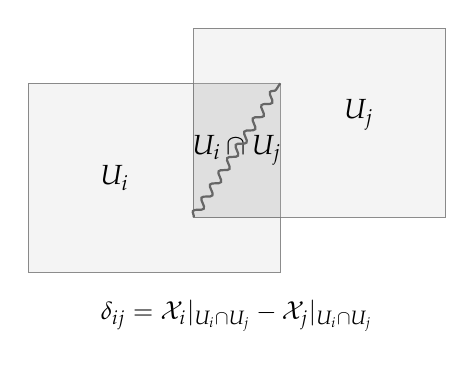
\begin{tikzpicture}[scale=1.0]
    \draw[patch] (0,0) rectangle (3.2,2.4);
    \draw[patch] (2.1,0.7) rectangle (5.3,3.1);
    \draw[overlap] (2.1,0.7) rectangle (3.2,2.4);
    \node at (1.1,1.2) {$U_i$};
    \node at (4.2,2.0) {$U_j$};
    \node at (2.65,1.55) {$U_i\cap U_j$};
    \draw[obstruction] (2.1,0.7) -- (3.2,2.4);
    \node[note] at (2.65,-0.55) {$\delta_{ij}=\X_i|_{U_i\cap U_j}-\X_j|_{U_i\cap U_j}$};
\end{tikzpicture}}
\caption{A nonzero overlap mismatch $\delta_{ij}$ defines a \v{C}ech 1-cochain; its cohomology class measures the obstruction to assembling local sections into a global field.}
\end{figure}

\subsection{Coarse-Graining as a Contravariant Functor}

Let $\mathcal{U}$ denote a fine cover and $\mathcal{V}$ a coarser cover of
spacetime. Coarse-graining induces a map $\pi : \mathcal{U} \to \mathcal{V}$
and therefore a morphism of sites. This defines a contravariant functor on
sheaves
\[
    \pi^* : \mathrm{Sh}(\mathcal{V}) \longrightarrow \mathrm{Sh}(\mathcal{U}),
\]
together with a pushforward
\[
    \pi_* : \mathrm{Sh}(\mathcal{U}) \longrightarrow \mathrm{Sh}(\mathcal{V}).
\]
The effective coarse-grained configuration is given by
$\overline{\mathcal{F}} := \pi_* \mathcal{F}$.

\begin{remark}
The functor $\pi_*$ integrates out fine-scale variability while preserving
global consistency data encoded in cohomology.
\end{remark}

\subsection{Derived Structure and Accessibility Collapse}

The configurational accessibility field $\Sfield$ governs the complexity of
the sheaf $\mathcal{F}$. In regimes of high $\Sfield$, the sheaf admits many
distinct local sections and nontrivial cohomology. As $\Sfield$ decreases,
admissible configurations are restricted and the sheaf simplifies: higher
cohomology groups become trivial, and the sheaf approaches one with fewer
generators and simpler gluing data.

\begin{proposition}
In the low-accessibility regime, higher cohomology groups of $\mathcal{F}$
collapse, and the sheaf becomes effectively locally constant with respect to
the coarse cover.
\end{proposition}

\subsection{Emergence of Bundle Geometry}

When cohomological obstructions are suppressed and the sheaf simplifies, the
remaining structure can be described by a fiber bundle. The sheaf
$\overline{\mathcal{F}}$ determines a base space given by spacetime, fibers
given by residual admissible configurations, and transition functions derived
from overlap data. The transport field $\mathbf{v}$ induces a connection on
this bundle, while variations in $\Phi$ generate curvature.

\begin{proposition}[Emergent Bundle Structure]
In the limit of strong accessibility collapse, the coarse-grained sheaf
$\overline{\mathcal{F}}$ determines a fiber bundle with connection, whose
curvature encodes the residual constraint structure of the system.
\end{proposition}

More precisely: in the limit $\Sfield \to 0$, the configuration sheaf admits
a unique global section, up to isomorphism, compatible with all overlaps, and
its residual symmetry reduces to a structure group acting on fibers. Bundle
geometry is therefore not assumed but is the terminal object of accessibility
collapse: the unique structure that remains when all admissible alternatives
have been foreclosed.

This construction provides a precise sense in which geometric unity emerges
from constrained dynamics. The bundle structure is not fundamental but arises
as the global organization of a sheaf of local configurations under
coarse-graining and accessibility collapse. Geometric unity corresponds to
the regime in which the configuration sheaf reduces to a bundle with
connection, and dynamics are governed by its associated curvature.

\subsection{Higher Sheaf Structure and Trajectory Memory}

In regimes of high configurational accessibility, the configuration sheaf
$\mathcal{F}$ should properly be regarded as a higher sheaf, or derived
stack, with nontrivial higher gluing data encoding trajectory memory.
The non-Markovian memory kernels $\mathcal{M}_i$ introduced in Section~8
represent precisely this higher data: they encode how local trajectory
fragments must be consistently assembled across overlaps in a way that a
1-sheaf, which tracks only field values and their immediate compatibility,
cannot capture. Accessibility collapse corresponds to truncation of this
higher sheaf to a 1-sheaf, as the system loses the topological diversity
that made higher gluing data necessary. The derived-to-classical transition
is therefore not merely a computational simplification but a structural
consequence of $\Sfield \to 0$: when few futures remain, the memory of
alternative pasts becomes irrelevant to global coherence.

\begin{proposition}[Bundle Emergence as Terminal Descent Object]
Let $\mathcal{F}$ be the configuration sheaf and suppose that for a coarse
cover $\mathcal{V}$, $\check{H}^k(\mathcal{V},\mathcal{F}) = 0$ for all
$k \geq 1$. Then $\mathcal{F}$ is equivalent to the sheaf of sections of a
fiber bundle with structure group $G$ acting on the residual admissible fiber.
\end{proposition}

This replaces the earlier philosophical statement with a standard descent
condition: bundle geometry is not assumed but is the unique structure that
remains once all higher cohomological obstructions have vanished.

\begin{remark}[Equivalence of Functional Regimes]
Up to coarse-graining, the following conditions are equivalent signatures of
functional lock-in: persistent low configurational accessibility $\Sfield$;
reduction in admissible homotopy classes; vanishing higher sheaf cohomology
$\check{H}^k = 0$ for $k \geq 1$; and emergence of a bundle description with
structure group $G$. This equivalence constitutes the unified interpretation
of function across all domains treated in the paper.
\end{remark}

% ============================================================
\section{Lorentz Transformations as Sheaf Automorphisms}
% ============================================================

The projection-based language developed above must remain consistent with
relativistic causality. In particular, it must not imply faster-than-light
propagation. This is ensured by the fact that Lorentz transformations act as
automorphisms of the projection functor from the configuration sheaf to observer
coordinate spaces, not on the underlying events or trajectories themselves.

\subsection{Invariant Structure}

In special relativity, the invariant object is the spacetime interval
$s^2 = c^2 t^2 - \|x\|^2$. Observers may disagree about temporal and spatial
coordinates, but they agree on the interval. Within the present framework, this
corresponds to an invariant admissibility condition on trajectories. A
trajectory $\gamma$ is not defined by a single observer's projection, but by the
equivalence class of all projections that preserve its invariant structure.

\subsection{Observers as Local Sections}

An observer corresponds to a local section of the configuration sheaf. Given a
trajectory $\gamma$, observer $\alpha$ assigns a projected representation
$\Pi_\alpha(\gamma) = (t_\alpha,x_\alpha)$, while observer $\beta$ assigns
$\Pi_\beta(\gamma) = (t_\beta,x_\beta)$. Both are representations of the same
underlying trajectory. A Lorentz transformation is therefore a map
\[
    \Lambda_{\alpha\beta} :
    \Pi_\alpha(\gamma) \longrightarrow \Pi_\beta(\gamma)
\]
that preserves the invariant interval.

\subsection{Lorentz Transformations as Automorphisms}

In sheaf-theoretic terms, Lorentz transformations act as automorphisms of the
sheaf of observer-projections, changing local coordinate descriptions while
preserving the global admissibility structure:
\[
    \Lambda_{\alpha\beta}^* \mathcal{I}[\gamma]
    =
    \mathcal{I}[\gamma].
\]
Thus Lorentz transformations deform the image of a trajectory under projection,
not the trajectory itself.

\subsection{Time Dilation as Projection Distortion}

For two events occurring at the same spatial location in the comoving frame,
the proper time is $\tau = t_0$. An observer who sees the system moving with
speed $v$ measures
\[
    t = \frac{t_0}{\sqrt{1-v^2/c^2}}.
\]
This does not mean that the event itself has changed. Rather, the same invariant
trajectory is being represented through a different section of the observer
sheaf. The standard light-clock derivation expresses this as
$(ct)^2 = (vt)^2 + (ct_0)^2$, so that $t = \gamma(v)t_0$ with
$\gamma(v) = (1-v^2/c^2)^{-1/2}$. The diagonal path is longer in the projected
image not because the underlying causal trajectory has become superluminal, but
because the observer's slicing has tilted relative to the intrinsic trajectory.

\subsection{No Superluminal Consequence}

A trajectory is admissible only if it is timelike or null:
$c^2t^2-\|x\|^2 \geq 0$. Because Lorentz transformations preserve this
quantity, they preserve causal type.

\begin{proposition}[No Superluminal Propagation]
If a trajectory is timelike or null in one frame, then it remains timelike or
null in every Lorentz-related frame. Therefore no Lorentz transformation can
convert a subluminal trajectory into a superluminal one.
\end{proposition}

\begin{proof}
Lorentz transformations preserve the spacetime interval. Since the sign of the
interval determines whether a trajectory is timelike, null, or spacelike, causal
classification is invariant under the transformation.
\end{proof}

Faster-than-light travel would require changing the invariant causal structure,
not merely changing the projection. Such a change is excluded by the framework.
Lorentz transformations deform the representation of a trajectory, not the
event or trajectory itself.

% ============================================================
\section{Lorentz Invariance from an RSVP-Style Trajectory Functional}
% ============================================================

We now show how the relativistic invariant can be expressed within the
constraint--transport--accessibility language of the present framework. The goal
is not to replace special relativity but to show that Lorentz invariance appears
as a symmetry of admissible trajectories.

\subsection{Trajectory Functional}

Let a trajectory through spacetime and configuration space be written as
\[
    \gamma : \tau \mapsto (x^\mu(\tau),\Phi(\tau),\mathbf{v}(\tau),\Sfield(\tau)),
\]
where $\tau$ denotes intrinsic progression along the trajectory. We define an
effective trajectory action coupling proper-time length to the RSVP fields:
\begin{align}
    \mathcal{A}_{\mathrm{RSVP}}[\gamma]
    &=
    \int\!\Bigl[
        \sqrt{c^2\dot{t}^{\,2}-\|\dot{\mathbf{x}}\|^2}
        + V_\Phi(\Phi)
        \notag\\
    &\qquad
        + \tfrac{1}{2}\mu(\Phi)\,g_{\mu\nu}v^\mu v^\nu
        - \lambda \Sfield
    \Bigr]d\tau,
    \label{eq:rsvp_action}
\end{align}
where $V_\Phi(\Phi)$ encodes structural constraint, $\mu(\Phi)g_{\mu\nu}v^\mu
v^\nu$ encodes transport cost, and $-\lambda\Sfield$ encodes configurational
accessibility.

\subsection{Admissibility Constraint}

Relativistic causality imposes $c^2\dot{t}^{\,2}-\|\dot{\mathbf{x}}\|^2 \geq 0$,
equivalently $\|\dot{\mathbf{x}}\| \leq c\dot{t}$. Thus admissible trajectories
are those whose spacetime projection is timelike or null. In RSVP language, the
physical transport component satisfies $\|\mathbf{v}_{\mathrm{phys}}\| \leq c$.

\subsection{Lorentz Symmetry of the Action}

Let $\Lambda$ be a Lorentz transformation. Then
$c^2dt^2-d\mathbf{x}^2 = c^2dt'^2-d\mathbf{x}'^2$, so the square root term in
equation~\eqref{eq:rsvp_action} is invariant. If $\Phi$ and $\Sfield$ are
treated as Lorentz scalars and $v^\mu$ as a four-vector, the full action is
invariant under $\Lambda$, giving the Lorentz-covariant form
\begin{align*}
    \mathcal{A}_{\mathrm{RSVP}}[\gamma]
    &=
    \int\!\bigl[
        ds
        + V_\Phi(\Phi)\,d\tau
        \\&\quad
        + \tfrac{1}{2}\mu(\Phi)\,g_{\mu\nu}v^\mu v^\nu\,d\tau
        - \lambda\Sfield\,d\tau
    \bigr],
\end{align*}
where $ds^2 = g_{\mu\nu}dx^\mu dx^\nu$.

\begin{proposition}[Lorentz Invariance of Admissible Trajectories]
The set of admissible RSVP trajectories is invariant under Lorentz
transformations whenever the RSVP action is constructed from Lorentz-scalar
field combinations.
\end{proposition}

\begin{proof}
Lorentz transformations preserve the Minkowski metric: $\Lambda^\top g \Lambda
= g$. Therefore $g_{\mu\nu}\dot{x}^\mu\dot{x}^\nu$ is invariant. Since
admissibility is defined by the sign of this quantity, the admissible set is
preserved. If the field couplings are Lorentz scalars, the action is also
invariant.
\end{proof}

\subsection{Time Dilation Recovered}

For a trajectory with spatial velocity $v$, the invariant interval gives
$d\tau^2 = dt^2(1-v^2/c^2)$, so $dt = d\tau(1-v^2/c^2)^{-1/2}$. The usual
Lorentz factor $\gamma(v) = (1-v^2/c^2)^{-1/2}$ is recovered. In the present
interpretation, $\gamma(v)$ measures projection distortion: the factor by which
an observer-section elongates the image of an invariant trajectory when that
trajectory has transverse transport relative to the frame.

% ============================================================
\section{Causality as a Sheaf-Theoretic Admissibility Constraint}
% ============================================================

The previous section established that Lorentz invariance arises as a symmetry
of admissible trajectories. We now refine this result by showing that causality
itself can be interpreted as a sheaf-theoretic constraint on the existence of
global sections.

\subsection{The Admissible Subsheaf}

For each open set $U \subset \Omega \times [0,T]$, define
\[
    \mathcal{F}_{\mathrm{adm}}(U)
    :=
    \left\{
        \X \in \mathcal{F}(U)
        \mid
        g_{\mu\nu}\dot{x}^\mu\dot{x}^\nu \geq 0
    \right\}.
\]
This defines a subsheaf $\mathcal{F}_{\mathrm{adm}} \subset \mathcal{F}$
consisting of locally admissible configurations. Stability under restriction
follows immediately: if $\X$ satisfies the causality constraint on $U$, its
restriction to any $V \subset U$ does also.

\subsection{Global Admissibility and Gluing}

A global trajectory exists if and only if a compatible family of local sections
$\{\X_i \in \mathcal{F}_{\mathrm{adm}}(U_i)\}$ can be glued into a single
section over $\bigcup_i U_i$. Gluing is obstructed if the local data implies
inconsistent causal structure across overlaps.

\begin{definition}[Causal Compatibility]
A family $\{\X_i\}$ is causally compatible if on each overlap $U_i \cap U_j$,
the induced trajectories agree both as fields and as elements of
$\mathcal{F}_{\mathrm{adm}}$.
\end{definition}

\begin{proposition}
A global admissible trajectory exists if and only if the associated
\v{C}ech 1-cocycle of mismatches vanishes in
$\check{H}^1(\{U_i\}, \mathcal{F}_{\mathrm{adm}})$.
\end{proposition}

\subsection{Exclusion of Superluminal Patching}

Suppose one attempts to construct a trajectory that is locally admissible in
each patch but globally superluminal. This would require that on overlaps
$U_i \cap U_j$, the local sections agree as fields but disagree in causal
classification. Such a mismatch would produce a nontrivial cohomology class
$[\delta] \neq 0$, preventing the existence of a global section.

\begin{proposition}[No Superluminal Gluing]
There exists no global section of $\mathcal{F}$ whose local restrictions are
timelike in each patch but collectively define a spacelike trajectory.
\end{proposition}

\begin{proof}[Sketch]
If such a section existed, it would define a global trajectory violating
$g_{\mu\nu}\dot{x}^\mu\dot{x}^\nu \geq 0$. However, local admissibility
enforces this inequality in each patch. Violation at the global level would
require inconsistent gluing, which is obstructed by the sheaf condition.
Therefore no such global section exists.
\end{proof}

Causality is therefore not merely a local inequality but a global consistency
condition on the sheaf of configurations. Superluminal motion would correspond
not to a different projection but to attempting to extend a locally admissible
section beyond the domain where the sheaf condition holds; the obstruction is
not energetic but categorical --- the extension fails to exist. The speed of
light is not a dynamical limit imposed on trajectories, but a structural
boundary enforced by the existence of global sections.

\begin{figure}[ht]
\centering
\resizebox{0.5\linewidth}{!}{%
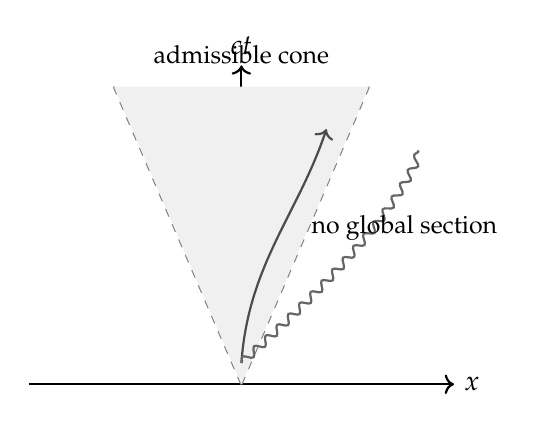
\begin{tikzpicture}[scale=0.9]
    \draw[axis] (0,0) -- (6,0) node[right] {$x$};
    \draw[axis] (3,0) -- (3,4.5) node[above] {$ct$};
    \draw[access] (3,0) -- (1.2,4.2);
    \draw[access] (3,0) -- (4.8,4.2);
    \fill[black!6] (3,0) -- (1.2,4.2) -- (4.8,4.2) -- cycle;
    \draw[fieldline] (3,0.3) .. controls (3.1,1.7) and (3.8,2.4) .. (4.2,3.6);
    \draw[obstruction] (3,0.3) .. controls (4.0,1.2) and (5.2,2.4) .. (5.5,3.3);
    \node[note] at (3,4.65) {admissible cone};
    \node[note] at (5.3,2.2) {no global section};
\end{tikzpicture}}
\caption{Superluminal patching fails because spacelike extension lies outside the admissible subsheaf. The causal boundary is a structural property of gluing, not a dynamical speed limit.}
\end{figure}

% ============================================================
\section{Projection Geometry and the Interpretation of Time Dilation}
% ============================================================

We now return to the interpretation of time dilation in light of the preceding
formalism.

\subsection{Trajectory Versus Representation}

Let $\gamma$ be a fixed admissible trajectory. Observers $\alpha$ and $\beta$
assign projections $\Pi_\alpha(\gamma) = (t_\alpha,x_\alpha)$ and
$\Pi_\beta(\gamma) = (t_\beta,x_\beta)$. These are not different trajectories
but different coordinate representations of the same object.

\subsection{Geometric Origin of Time Dilation}

The light-clock construction yields $(ct)^2 = (vt)^2 + (ct_0)^2$, which implies
$t = \gamma(v)t_0$. This relation is geometric: it arises from the metric
structure of spacetime. In the present framework, it reflects the fact that
projection operator $\Pi_\alpha$ slices the trajectory at an angle relative to
$\Pi_\beta$. Let intrinsic progression along $\gamma$ be parameterized by
$\tau$, so $d\tau^2 = dt^2 - dx^2/c^2$. Transport through the vector field
$\mathbf{v}$ introduces transverse components in the projected representation,
increasing the apparent length of the trajectory. Observed time is the length
of a projected trajectory; proper time is the intrinsic length of the trajectory
itself.

\subsection{No Physical Slowing of Time}

This resolves the common misconception that time slows down for moving objects.
The trajectory $\gamma$ does not change, the invariant length $\tau$ does not
change, and only the projection changes. Time dilation is not a change in
physical evolution but a change in how that evolution is represented.

The projection-based interpretation is therefore conservative with respect to
relativity. The same admissible trajectory is seen differently by different
observers, but its causal and geometric structure remains unchanged. This aligns
naturally with the broader framework: projection operators $\Pi_k$ correspond to
observers, sheaf structure encodes consistency across projections, and trajectory
invariants define admissibility.

% ============================================================
\section{Metric Curvature from Spatial Variation of Constraint}
% ============================================================

The preceding sections treated Lorentz invariance in the flat-spacetime limit,
where admissible trajectories are governed by a fixed Minkowski metric. We now
indicate how the same framework extends toward curved spacetime by allowing the
constraint field $\Phi$ to modify the effective metric experienced by
trajectories.

\subsection{From Fixed Metric to Effective Metric}

In special relativity, admissibility is defined by
$\eta_{\mu\nu}\dot{x}^\mu\dot{x}^\nu \geq 0$, where $\eta_{\mu\nu}$ is the
Minkowski metric. In a constrained-field setting, the scalar field $\Phi(x)$ may
alter the local geometry of admissibility. We therefore introduce an effective
metric
\[
    g_{\mu\nu}^{\mathrm{eff}}(x)
    =
    g_{\mu\nu}\bigl(\Phi(x),\nabla\Phi(x),\Sfield(x)\bigr),
\]
so that causal admissibility becomes
$g_{\mu\nu}^{\mathrm{eff}}(x)\dot{x}^\mu\dot{x}^\nu \geq 0$. The effective
metric is not identified with the constraint field itself but arises as the
unique, up to equivalence, local bilinear form compatible with admissibility
under the constraint--transport--accessibility coupling. Curvature arises from
spatial variation in the constraint structure rather than being imposed
externally. In the flat limit $\Phi = \mathrm{const}$,
$g_{\mu\nu}^{\mathrm{eff}} \to \eta_{\mu\nu}$, recovering special relativity.

\subsection{Constraint Gradients as Curvature Sources}

If $\Phi$ varies slowly, write the effective metric as a perturbation of the
flat metric: $g_{\mu\nu}^{\mathrm{eff}} = \eta_{\mu\nu} + h_{\mu\nu}[\Phi]$,
where to lowest order
\[
    h_{\mu\nu}[\Phi]
    =
    a\,\Phi\,\eta_{\mu\nu}
    +
    b\,\partial_\mu\Phi\,\partial_\nu\Phi
    +
    c\,\nabla_\mu\nabla_\nu\Phi,
\]
for phenomenological coefficients $a,b,c$. The first term rescales local
interval structure, the second introduces directional anisotropy from gradients
of constraint, and the third encodes curvature-like response to second-order
spatial variation.

\subsection{Geodesics as Constraint-Compatible Trajectories}

Given the effective metric, admissible free trajectories extremize the
proper-time functional $\tau[\gamma] = \int_\gamma \sqrt{g_{\mu\nu}^{\mathrm{eff}}dx^\mu dx^\nu}$.
The resulting equations are the geodesic equations
\[
    \frac{d^2 x^\mu}{d\tau^2}
    +
    \Gamma^\mu_{\alpha\beta}
    \frac{dx^\alpha}{d\tau}
    \frac{dx^\beta}{d\tau}
    =
    0,
\]
where $\Gamma^\mu_{\alpha\beta}$ are the Christoffel symbols of
$g_{\mu\nu}^{\mathrm{eff}}$. In the constrained-field interpretation, these are
trajectories of least distortion through the admissibility geometry determined
by $\Phi$. Gravitational curvature corresponds to spatial variation in the
geometry of admissibility.

\subsection{Relation to the Einstein Field Equations}

A complete recovery of general relativity would require specifying the dynamical
relation between $\Phi$ and the effective metric. Formally, one may introduce an
action
\[
    \mathcal{A}
    =
    \int
    \left[
        \frac{1}{16\pi G}R(g^{\mathrm{eff}})
        +
        \mathcal{L}_{\Phi,\mathbf{v},\Sfield}
        +
        \mathcal{L}_{\mathrm{matter}}
    \right]
    \sqrt{-g^{\mathrm{eff}}}\,d^4x,
\]
where $R(g^{\mathrm{eff}})$ is the scalar curvature. Variation with respect to
$g^{\mathrm{eff}}_{\mu\nu}$ gives equations of the form
\[
    G_{\mu\nu}(g^{\mathrm{eff}})
    =
    8\pi G
    \left(
        T_{\mu\nu}^{\mathrm{matter}}
        +
        T_{\mu\nu}^{\Phi,\mathbf{v},\Sfield}
    \right),
\]
where $T_{\mu\nu}^{\Phi,\mathbf{v},\Sfield}$ represents the contribution of
constraint, transport, and accessibility fields to the effective geometry.

\subsection{Weak-Field Limit}

In the weak-field, slow-motion limit, $g_{00}^{\mathrm{eff}} \approx 1 +
2\varphi/c^2$, where $\varphi$ is the Newtonian gravitational potential. In the
constrained-field interpretation, $\varphi$ may be modeled as a coarse-grained
projection of $\Phi$: $\varphi = \mathcal{P}[\Phi]$ for some projection or
averaging operator $\mathcal{P}$. The geodesic equation then reduces to
$d^2\mathbf{x}/dt^2 = -\nabla\varphi$, so gravitational acceleration appears as
motion along gradients of the projected constraint field.

\subsection{No Violation of Relativistic Causality}

Because admissibility is still defined by
$g_{\mu\nu}^{\mathrm{eff}}\dot{x}^\mu\dot{x}^\nu \geq 0$, curvature does not
permit superluminal propagation. It changes the structure of admissible
trajectories but does not remove the causal boundary.

\begin{proposition}[Curved Causal Admissibility]
If the effective metric $g_{\mu\nu}^{\mathrm{eff}}$ is Lorentzian, then causal
classification remains well-defined locally, and admissible trajectories remain
timelike or null with respect to $g^{\mathrm{eff}}$.
\end{proposition}

\begin{proof}
A Lorentzian metric defines a local light cone at each point. Curvature changes
the orientation and structure of cones across spacetime, but not the local
distinction between causal and noncausal directions.
\end{proof}

The passage from special to general relativity is therefore interpreted as the
transition from a fixed admissibility geometry to a spatially varying one:
$\eta_{\mu\nu} \longrightarrow g_{\mu\nu}^{\mathrm{eff}}(\Phi,\nabla\Phi,\Sfield)$.
Special relativity corresponds to the case where $\Phi$ is uniform and the
admissibility geometry is flat; general relativity corresponds to the case where
the geometry of admissibility varies across spacetime. Curvature is the
deformation of the admissibility geometry induced by nonuniform constraint.

% ============================================================
\section{A Causal Example: Collagen Peptide Gelation}
% ============================================================

Consider a collagen peptide network undergoing gelation in aqueous solution.
The experimental objective is to determine whether an imposed preparation
variable---ionic strength---causally changes the final mechanical stiffness of
the network, and whether this effect is mediated by mesoscale changes in
aggregation, fiber bundling, and transport accessibility.

Let the treatment variable be $A \in \{a_0,a_1\}$, where $a_0$ denotes a
low-ionic-strength condition and $a_1$ denotes a high-ionic-strength condition.
Let the observed outcome be the storage modulus $Y = G'$ measured after gelation
by oscillatory rheology. The causal estimand is the average treatment effect
\[
    \tau
    =
    \mathbb{E}\!\left[Y(a_1)-Y(a_0)\right],
\]
where $Y(a)$ denotes the stiffness that would be observed if the system were
prepared under condition $a$.

Within the constrained-field framework, the treatment does not act directly on
$Y$. Instead, it perturbs the field evolution, writing
$\X(x,t;A) = \bigl(\Phi(x,t;A),\mathbf{v}(x,t;A),\Sfield(x,t;A)\bigr)$.
Here $\Phi$ represents collagen peptide aggregation and local fiber density,
$\mathbf{v}$ represents transport and alignment during gelation, and $\Sfield$
represents configurational accessibility. Ionic strength modifies the local
interaction term $f_{\mathrm{loc}}(\Phi;A)$ in the free-energy functional,
altering which aggregates nucleate, how rapidly fibers bundle, how transport
pathways close, and when the system loses configurational accessibility. The
treatment therefore acts upstream of structure. The final modulus is the
mechanical expression of a completed trajectory, specifically one that has
entered a low-$\Sfield$ regime in which configurational accessibility has
collapsed and network rearrangement is no longer dynamically available:
\[
    G'
    =
    \mathcal{R}
    \left[
        \{\Phi(t),\mathbf{v}(t),\Sfield(t)\}_{t=0}^{T}
    \right].
\]

\subsection{Trajectory Dependence and TARTAN}

Collagen peptide networks are path-dependent. Two samples may have similar
final density but different assembly histories, leading to different network
topology and stiffness. Instead of summarizing the system only by
$\Phi(\cdot,T)$, we cover the gelation trajectory by overlapping temporal
patches $U_i = [t_i,t_{i+1}]$, assign to each patch a local field history
$\X_i$, and enforce overlap consistency. This prevents the model from treating
gelation as a Markovian sequence of unrelated snapshots. Early nucleation,
intermediate bundling, and late network locking are represented as overlapping
trajectory fragments with a history-consistency score
\[
    H_k
    =
    \sum_i
    \|\X_{i,k}-\widehat{\X}_{i,k}\|^2
    +
    \sum_{i,j}
    \|\rho_{ij}(\X_{i,k})-\rho_{ji}(\X_{j,k})\|^2.
\]

\subsection{Statistical Model}

A practical regression model is
\[
    G'_k
    =
    \beta_0
    +
    \beta_A A_k
    +
    \int_0^T
    \beta_M(t)\,M_k(t)\,dt
    +
    \beta_H H_k
    +
    \epsilon_k,
\]
where $k$ indexes samples, $M_k(t) = (\xi(t), r_f(t), \alpha(t), c(t))$
contains measured structural summaries (correlation length, fiber radius,
anisotropy index, connectivity), and $H_k$ is the history-consistency score.
A significant $\beta_A$ after adjustment for $M(t)$ and $H$ indicates a
direct effect of ionic strength not explained by observed structure. A
significant $\beta_H$ indicates that assembly history contributes to stiffness
beyond static morphology---precisely the regime where trajectory-aware
representation is indispensable.

\subsection{Testing for Accessibility Collapse}

The constraint-induced collapse mechanism in equation~\eqref{eq:S_evo} predicts
that ionic strength changes the rate at which the system enters a low-$\Sfield$
regime. This can be tested by designing two preparation protocols that produce
similar final scattering profiles but different assembly paths---for example,
one condition rapidly screening electrostatic repulsion early in gelation, another
gradually increasing ionic strength. If the final $\Phi(\cdot,T)$ appears similar
but the measured moduli differ, the network carries non-Markovian memory and
the assembly path has causal relevance. The corresponding statistical test adds
$\beta_H H_k$ to a baseline model containing only final-structure summaries;
significance of $\beta_H$ after this adjustment would confirm that $\Sfield$
history, not just $\Phi$ geometry, determines function.

% ============================================================
\section{Implications for Experiment and Design}
% ============================================================

The unified framework has direct consequences for how mesoscale systems are
studied and engineered. The emphasis shifts from identifying stable structures
and correlating them with properties to controlling trajectories in
configuration space.

\paragraph{Design as trajectory control.}
Because function corresponds to stabilized evolution of $\X(x,t)$ within a
low-$\Sfield$ basin, design becomes the problem of steering the system into a
desired dynamical regime. Let $\mathcal{U}$ denote a set of admissible controls
(temperature, ionic strength, shear, chemical inputs). Then the design problem
can be formulated as
\[
    \min_{u(\cdot) \in \mathcal{U}}
    \;
    \mathcal{J}\bigl[\X(\cdot;u)\bigr],
\]
where $\mathcal{J}$ is an objective functional encoding desired outcomes such
as mechanical strength, conductivity, or permeability. Unlike classical
optimization over static configurations, this formulation optimizes over
trajectories in configuration space.

From this perspective, the design of functional materials can be interpreted as
the controlled reduction of configurational accessibility along specific
trajectories. Processes such as cross-linking, crystallization, alignment, and
templating may be viewed as mechanisms for inducing accessibility collapse in
targeted regions of configuration space. Biological systems achieve similar
effects through sequence-encoded folding pathways and cooperative assembly.
While this interpretation is not exhaustive, it provides a unifying lens through
which diverse fabrication and selection processes can be understood.

\paragraph{Experimental strategy.}
Experiments should be structured to probe sensitivity to trajectory rather than
only final state. Key strategies include time-resolved measurements such as SAXS,
SANS, and microscopy \cite{hamley2023,akepati2026}; controlled perturbations
during evolution; comparison of protocols yielding similar final structure but
different histories; and reconstruction of trajectory patches from partial
observations. These approaches align naturally with the projection framework
described in Section~9 and the trajectory-aware representation of Section~8.

\paragraph{Cross-domain transfer.}
Because the governing structure is shared, insights from one domain can be
transferred to another. Methods developed to control anisotropy in polymer
networks may inform the design of biological scaffolds, while interfacial
stabilization strategies in emulsions may inform membrane engineering.

\begin{proposition}[Transferability]
If two systems are governed by functionals of similar form, then control
strategies that modify trajectories in one system can be adapted to the other
under appropriate scaling.
\end{proposition}

% ============================================================
\section{Modular Externalization, Residue Reuse, and State-Space Expansion}
% ============================================================

The constrained-field framework developed for mesoscale physical systems
admits a direct extension to socio-technical and computational systems. In
these domains, the fields $(\Phi,\mathbf{v},\Sfield)$ do not represent
material aggregation and transport alone, but organizational constraint,
workflow propagation, and the space of admissible transformations across
distributed systems.

\subsection{Modularization as Constraint Redistribution}

Modern systems---software platforms, economic networks, and institutional
structures---are characterized by modular decomposition. A complex process is
partitioned into subcomponents, each governed by local rules and interfaces.
Within the present framework, this corresponds to a redistribution of the
constraint field $\Phi$ across system boundaries.

\begin{definition}[Modular Externalization]
A system externalizes constraint when it partitions a global process into
modules $\{U_i\}$ such that each module carries a localized constraint field
$\Phi_i$, while inter-module interactions are mediated through reduced
interface constraints.
\end{definition}

This operation does not eliminate constraint; it relocates it. The internal
complexity of a module may decrease, but the global system inherits new
dependencies encoded in the overlap conditions between modules. In sheaf-
theoretic terms, modularization replaces a single global section with a
collection of local sections whose compatibility must be enforced across
interfaces.

\subsection{Residue as Latent Admissible Structure}

A characteristic feature of modular systems is the production of byproducts:
unused computation, data exhaust, waste heat, or partially completed
transformations. These residues are often treated as inefficiencies, yet in
many systems they become inputs to new processes.

\begin{definition}[Admissible Residue]
A residue is admissible if it can be reinterpreted as a valid input to a
distinct transformation without violating the constraint structure of the
receiving module.
\end{definition}

Admissible residues function as latent trajectory fragments. Within the
trajectory-aware representation, they correspond to partial paths in
configuration space that were not completed within one module but remain
consistent with admissibility conditions elsewhere. Reuse of residue is
therefore equivalent to reattaching previously discarded trajectory segments
into new admissible paths.

\subsection{Orthograde Transformations and Low-Interference Directions}

New transformations in modular systems preferentially arise along directions
that do not disrupt existing constraint structures.

\begin{definition}[Orthograde Transformation]
A transformation is orthograde if it extends system functionality along a
direction that preserves local admissibility and minimizes interference with
existing constraint fields.
\end{definition}

Orthograde transformations correspond to low-coupling directions in the space
of admissible fluxes $\mathbf{v}$. They are the directions along which new
modules, services, or processes can be added without requiring global
reconfiguration. In algebraic terms, they approximate orthogonality with
respect to the bilinear form induced by the constraint structure.

\subsection{Local Constraint Reduction and Global State Expansion}

A central consequence of modular externalization is a divergence between local
and global measures of complexity.

\begin{proposition}[Local Constraint, Global Expansion]
Modular systems reduce local configurational uncertainty while expanding the
global space of admissible configurations through recombination of modules
and admissible residues.
\end{proposition}

\begin{proof}[Heuristic Argument]
Each module imposes constraints that reduce local $\Sfield$. However, the
composition of modules introduces combinatorial degrees of freedom: admissible
configurations correspond to compatible selections across modules. If residues
remain admissible, they introduce additional partial trajectories that can be
recombined, increasing the effective global $\Sfield$ even as local values
decrease.
\end{proof}

This result does not violate thermodynamic principles. Rather, it reflects a
redistribution of accessibility: uncertainty-like measures decrease locally due
to constraint, while the number of globally reachable configurations increases
through combinatorial composition. Systems compete by minimizing their own
constraint cost while increasing the total space of recomposable trajectories
they can access or control, which is why platform structures consistently
outperform point-solutions: they do not merely optimize a process but own the
adjacency structure of possible processes.

\subsection{Failure Modes: Non-Admissible Externalization}

Not all externalization produces beneficial expansion. If residues cannot be
reintegrated because they violate admissibility conditions or require
prohibitive reconstruction, then they do not contribute to global state-space
growth.

\begin{proposition}[Dead Residue]
Residues that cannot be embedded into admissible trajectories act as sinks of
configurational accessibility and do not contribute to functional expansion.
\end{proposition}

Such residues correspond to irrecoverable waste, technical debt, or
incompatible interfaces. They increase local disorder without expanding the
global space of useful configurations, and therefore degrade system
functionality. The distinction between productive and dead externalization is
whether the residue remains admissible for recombination---the difference
between a data exhaust pipeline and pollution, or between reusable abstractions
and technical debt.

% ============================================================
\section{Recency, Locality, and the Bitter Lesson}
% ============================================================

The trajectory-aware framework provides a structural account of recency
weighting---a ubiquitous heuristic in learning systems, caching architectures,
and human cognition---and connects it to the empirical observation that
large-scale, compute-driven learning methods systematically outperform methods
that rely on hand-crafted structure.

\subsection{Recency as Local Admissibility Projection}

In the RSVP framework, the admissibility log $\mathcal{L}$ maintains a full
record of past events. Full reconstruction from this log is, in general,
expensive: it requires evaluating global gluing consistency across the entire
history. Recency weighting provides a low-cost approximation by assigning
\[
    \mathrm{weight}(e_k) \propto e^{-\lambda(t_n - t_k)},
\]
discarding events beyond an effective horizon. This is not merely a heuristic.
More recent events sit inside the current admissible basin, have not yet been
invalidated by constraint evolution, and are more likely to glue consistently
with the current local section of the configuration sheaf. Recency weighting
therefore approximates the projection of the full admissibility log onto the
current local tangent space of valid trajectories.

\begin{proposition}[Recency as Local Admissibility Projection]
Time-weighted recency bias approximates the projection of the admissibility
log onto the locally coherent trajectory subspace, minimizing gluing
obstructions and enabling stable real-time inference.
\end{proposition}

Older events are more likely to lie in different homotopy classes from the
current trajectory; newer events are more likely to be locally compatible.
Recency therefore minimizes expected gluing failure by discarding high-cost,
low-relevance historical branches. Responsiveness---the property of a system
that updates reliably under new information---is in this sense inversely
proportional to expected gluing failure.

\begin{proposition}[Recency as Minimal Obstruction Estimator]
Let $\mathcal{L}$ be an admissibility log and let $\widehat{\mathcal{L}}_\tau$
be its truncation to the interval $[t-\tau,t]$. Under a decay condition on
constraint evolution---specifically, that older events are exponentially less
likely to remain in the current admissible basin---the truncated log
$\widehat{\mathcal{L}}_\tau$ minimizes expected gluing obstruction among all
fixed-length summaries of $\mathcal{L}$.
\end{proposition}

This ties the recency heuristic directly to gluing optimality: exponential
weighting is not arbitrary but is the natural choice when constraint fields
evolve with bounded relaxation rate.

\subsection{Locality Constraints and Scaling Behavior}

Sutton's Bitter Lesson establishes that methods which scale with compute and
data consistently outperform methods that rely on handcrafted structure. The
RSVP interpretation of this result is as follows. Hand-crafted structure
corresponds to hard-coded constraints on admissible trajectories: the system's
configuration space is pre-restricted by design. Scalable methods instead
explore a broad trajectory space with weak priors, allowing structure to emerge
from data.

The difficulty is that broad exploration drives $\Sfield$ toward high values:
many trajectories remain admissible, optimization becomes unstable, and signal
is diluted by combinatorial expansion. Recency weighting resolves this by
imposing a locality constraint: the effective trajectory space is truncated to
a recent neighborhood, preserving local coherence without reverting to
hand-crafted global structure.

\begin{proposition}[Scaling Compatibility via Locality]
Systems that maintain performance under scale do so by enforcing locality
constraints---such as recency weighting---that bound effective configurational
accessibility, preserving tractable trajectory coherence as global capacity
increases.
\end{proposition}

The Bitter Lesson therefore requires two ingredients, not one. Exploration
capacity increases $\Sfield$ globally; locality constraints prevent $\Sfield$
from becoming computationally intractable locally. Recency bias is the simplest
possible locality operator that respects causal structure. This same pattern
appears in transformer attention, which implements soft recency weighting across
context; in reinforcement learning replay buffers, which prioritize recent and
high-return transitions; and in human working memory, which is capacity-limited
and recency-biased. These are all approximations to the same principle: retain
only the portion of the trajectory that still lies within the current admissible
basin.

% ============================================================
\section{A Minimal Synchronization Model of Cosmological Structure}
% ============================================================

Before developing the full five-dimensional model, we state a minimal,
parameter-free version that makes falsifiable predictions without free
functions. This version is the benchmark against which the richer model is
compared.

\subsection{Definition of the Synchronization Field}

We define a higher-dimensional binary coherence field
\[
    \sigma : \mathbb{R}^3 \times \mathbb{R} \times \Xi \to \{-1,+1\},
\]
where $\Xi$ is a compact internal dimension indexing coherence modes. The
observable scalar constraint field is the normalized projection
\[
    \Phi(x,t) = \frac{1}{|\Xi|} \int_{\Xi} \sigma(x,t,\xi)\,d\xi.
\]
The vector transport field arises from phase gradients:
$\mathbf{v}(x,t) = -\nabla\Phi(x,t)$. Configurational accessibility is defined
by local internal disagreement:
$\Sfield(x,t) = \log(1 + \operatorname{Var}_\xi[\sigma(x,t,\xi)])$.

\subsection{Parameter-Free Evolution Law}

The synchronization field evolves by nearest-neighbor alignment in the extended
space $\mathbb{R}^3 \times \Xi$:
\[
    \partial_t \sigma(x,\xi)
    =
    \operatorname{sign}\!\bigl(
        \Delta_x \sigma(x,\xi)
        +
        \Delta_{\xi} \sigma(x,\xi)
    \bigr).
\]
This defines a 5D Ising-type model with no tunable coupling constants beyond
lattice scale and time normalization.

\subsection{Scale-Free Coherence and Flat Rotation Curves}

Define the effective potential $\varphi_{\mathrm{eff}}(r) = \Phi(r)$. For
circular motion, $v_{\mathrm{rot}}^2(r) = r|d\Phi/dr|$. The only radial profile
with no preferred length scale and nonzero radial flux is logarithmic:
\[
    \Phi(r) = A\log(r/r_0),
    \qquad
    \frac{d\Phi}{dr} = \frac{A}{r},
    \qquad
    v_{\mathrm{rot}}^2 = A.
\]
Hence $v_{\mathrm{rot}} = \sqrt{A}$, a constant independent of $r$.

\subsection{Baryonic Tully--Fisher Scaling}

Define the total baryonic source strength $M_b = \int\rho_b\,d^3x$. Under the
minimal assumption that coherence charge $Q_\Phi \propto M_b$, and that the
radial coherence amplitude satisfies $A \sim Q_\Phi^{1/2}$, we obtain
$v_{\mathrm{rot}}^2 \propto M_b^{1/2}$, hence
\[
    v_{\mathrm{rot}}^4 \propto M_b.
\]
This recovers the baryonic Tully--Fisher relation without inserting a dark
matter halo profile or empirical interpolation function. The flatness of
rotation curves and the baryonic scaling both arise from scale-free coherence
geometry.

\subsection{Lensing Prediction}

Define the effective metric perturbation $g_{00} = -(1+2\Phi)$,
$g_{ij} = (1-2\Phi)\delta_{ij}$. The lensing potential is then directly
$\Phi$, and lensing maps correlate with coherence structure rather than
strictly with baryonic mass.

\subsection{Falsification Criteria}

The minimal model makes three parameter-free predictions. First, asymptotically
flat rotation curves arise without halo profile tuning; deviations in galaxies
with confirmed scale-free coherence environments falsify the model. Second, the
non-Markovian gravitational response satisfies $\partial_t\Phi \neq 0$ after a
perturbation to $\rho_b$, with a finite coherence relaxation time. Third,
lensing correlates with coherence domains rather than strictly baryonic density,
producing measurable deviations from $\Lambda$CDM in offset systems. Failure of
any condition falsifies the synchronization model as stated.

% ============================================================
\section{A Synchronization-Based Cosmological Extension}
% ============================================================

The constrained-field framework developed thus far admits a natural extension
to cosmological structure formation by interpreting the scalar constraint field
$\Phi$ as the coarse-grained projection of a higher-dimensional synchronization
process. In this section, we formalize this extension as a five-dimensional
Ising-like system whose coarse-grained dynamics reproduce the mesoscale field
equations introduced earlier.

\subsection{Underlying Synchronization Field}

Let spacetime be augmented by an additional internal coordinate $\xi$,
representing a coherence or synchronization dimension. The fundamental degrees
of freedom are binary variables $\sigma(x,t,\xi) \in \{-1,+1\}$. We define a
Hamiltonian
\begin{align*}
H[\sigma]
&= - J \!\sum_{\langle x,x' \rangle,\xi}\! \sigma(x,\xi)\sigma(x',\xi)\\
&\quad - K \!\sum_{x,\langle \xi,\xi' \rangle}\! \sigma(x,\xi)\sigma(x,\xi')\\
&\quad - \lambda \!\sum_{x,\xi} \sigma(x,\xi)\,\mathcal{E}(x),
\end{align*}
where $J$ is the spatial coupling governing structure formation, $K$ is the
coherence coupling governing synchronization strength, and $\mathcal{E}(x)$
is an external bias encoding baryonic matter and radiation. The dynamics follow
a stochastic relaxation process consistent with detailed balance.

\subsection{Projection to Mesoscale Fields}

The observable fields $(\Phi,\mathbf{v},\Sfield)$ arise as coarse-grained
projections of $\sigma$. The structural field is defined as the coherence
average $\Phi(x,t) = \langle \sigma(x,t,\xi) \rangle_\xi$. The transport field
emerges from spatial gradients of coherence: $\mathbf{v}(x,t) = -\mu(\Phi)\,
\nabla\Phi(x,t)$. The configurational accessibility field is defined by the
logarithmic density of admissible microstates: $\Sfield(x,t) = \log\Omega(x,t)$,
where $\Omega$ counts spin configurations consistent with local constraints.

\subsection{Continuum Limit and Effective Field Theory}

Under coarse-graining, the spin system admits a continuum description in terms
of a free-energy functional
\[
\F[\Phi]
=
\int_\Omega
\left[
-\frac{a}{2}\Phi^2
+ \frac{b}{4}\Phi^4
+ \frac{\kappa}{2}|\nabla\Phi|^2
\right] dx,
\]
recovering the Landau--Ginzburg structure of the mesoscale framework. The
resulting evolution equation
\[
\partial_t \Phi
=
D\Delta\Phi - a\Phi - b\Phi^3 + \gamma|\nabla\Phi|^2 + \eta
\]
defines the effective large-scale dynamics and provides the bridge between
discrete coherence states and continuous mesoscale behavior. Regions of high
$|\Phi|$ correspond to synchronized domains, projecting into observable
spacetime as galaxies and clusters. Interfaces between domains appear as
filaments and void boundaries.

% ============================================================
\section{Cosmological Predictions from Synchronization Dynamics}
% ============================================================

The synchronization-based extension yields physical predictions that differ
qualitatively from those of $\Lambda$CDM and from modified-gravity approaches
such as MOND.

\subsection{Galaxy Formation as Domain Coarsening}

In the absence of strong external bias, the synchronization field undergoes
spontaneous symmetry breaking followed by domain coarsening. The characteristic
domain size grows as $L(t) \sim t^{1/2}$, consistent with the Allen--Cahn
universality class.

\begin{proposition}[Galaxies as Coherence Domains]
Galaxies correspond to spatial regions in which the synchronization field $\Phi$
has converged to a locally stable phase, forming a coherent domain of low
configurational accessibility.
\end{proposition}

The characteristic size of a galaxy is therefore determined by the correlation
length of the synchronization field rather than by virial mass alone.

\subsection{Filamentary Structure as Domain Boundaries}

\begin{proposition}[Filaments as Phase Boundaries]
Cosmic filaments arise as domain walls of the synchronization field, representing
boundaries between regions of distinct phase alignment.
\end{proposition}

Unlike in $\Lambda$CDM, where filaments are conduits of matter flow into halos,
here they are topological features of the coherence field itself. Matter
distribution follows these structures but does not generate them.

\subsection{Rotation Curves from Coherence Coupling}

Define the spatial correlation function $C(r) = \langle\sigma(0)\sigma(r)\rangle$.
The effective rotational velocity is proportional to $v(r) \propto v_0\,C(r)$.
If coherence decays slowly, $C(r) \sim r^{-\epsilon}$, then $v(r) \approx
\mathrm{const}$.

\begin{proposition}[Flat Rotation from Long-Range Coherence]
Slow decay of synchronization correlations produces asymptotically flat rotation
curves independent of baryonic mass distribution.
\end{proposition}

\subsection{Environmental Dependence}

\begin{proposition}[Environmental Coherence Effect]
Galaxies embedded in regions of higher large-scale synchronization exhibit
enhanced rotational support relative to isolated galaxies of similar baryonic
mass.
\end{proposition}

This predicts correlations between rotation curve shape and position within the
cosmic web, providing a direct observational test not available in MOND.

\subsection{Memory Effects and Dwarf Galaxy Variability}

Because the synchronization field evolves through domain coarsening with
residual metastability, it retains memory of formation history. Post-merger
systems may exhibit long-lived deviations from equilibrium predictions. Small
systems are more sensitive to fluctuations in $\Phi$, predicting increased
scatter in velocity dispersion for dwarf galaxies without requiring additional
dark matter components.

% ============================================================
\section{Gravitational Lensing from Synchronization-Induced Effective Geometry}
% ============================================================

The synchronization-based extension must reproduce not only galaxy rotation
curves but also gravitational lensing. In the present framework, curvature is
not fundamental but emerges from spatial variation in $\Phi$.

\subsection{Effective Metric from Coherence Fields}

We postulate that the observable spacetime metric arises as a functional of the
synchronization field and its derivatives:
\[
g_{\mu\nu}^{\mathrm{eff}}(x)
=
\eta_{\mu\nu}
+
h_{\mu\nu}[\Phi(x),\nabla\Phi(x),\Sfield(x)],
\]
where to lowest nontrivial order
$h_{\mu\nu} = a\,\Phi\,\eta_{\mu\nu} + b\,\partial_\mu\Phi\,\partial_\nu\Phi
+ c\,\nabla_\mu\nabla_\nu\Phi$. The effective metric is not identified with
the constraint field itself but arises as the unique, up to equivalence, local
bilinear form compatible with admissibility under the coupling. In the flat
limit $\Phi = \mathrm{const}$, $g_{\mu\nu}^{\mathrm{eff}} \to \eta_{\mu\nu}$.

\subsection{Null Geodesics and Light Propagation}

Light propagation is determined by null geodesics of $g_{\mu\nu}^{\mathrm{eff}}$.
In the weak-field limit, write $g_{00}^{\mathrm{eff}} \approx 1 + 2\varphi/c^2$
and $g_{ij}^{\mathrm{eff}} \approx -(1-2\psi/c^2)\delta_{ij}$. The effective
potentials are $\varphi \sim \alpha\Phi + \beta|\nabla\Phi|^2$ and
$\psi \sim \alpha'\Phi$. The bending angle of light is then
\[
\hat{\alpha}
=
\frac{2}{c^2}
\int \nabla_\perp(\varphi+\psi)\,dz,
\]
so lensing depends on both the magnitude and spatial variation of $\Phi$, not
directly on mass density.

\begin{proposition}[Lensing from Coherence Gradients]
Gravitational lensing is dominated by spatial gradients of the synchronization
field. Galaxy clusters correspond to coherence peaks, filaments to strong
gradient regions, and voids to low-coherence regions with weak lensing.
\end{proposition}

\subsection{Recovery of the Standard Weak Lensing Limit}

Assuming baryonic matter induces a bias $\Delta\Phi \sim \rho_{\mathrm{baryon}}$,
one recovers $\Delta\varphi \sim \rho_{\mathrm{baryon}}$ to leading order,
reproducing Newtonian lensing in the regime where coherence is tightly coupled
to matter. Deviations arise when synchronization extends beyond the baryonic
distribution, producing apparent lensing not attributable to visible mass.

Relative to $\Lambda$CDM, the same observational effect attributed to dark
matter halos arises here from extended coherence fields. Relative to MOND, the
synchronization framework naturally produces lensing through the same mechanism
that generates rotation curves, without requiring a separate relativistic
extension.

% ============================================================
\section{Closure Relation and Forward Observational Model}
% ============================================================

The central unresolved degree of freedom in the synchronization framework is
the mapping between baryonic matter density $\rho_b$ and the coherence field
$\Phi$. To recover both dynamical and lensing observables, this mapping must
simultaneously reproduce Newtonian gravity in the high-density limit, generate
extended coherence beyond baryonic support for dark-like effects, and remain
stable under the dissipative dynamics of the RSVP equations.

\subsection{Field Equation for $\Phi$}

We postulate a nonlinear elliptic equation
\begin{equation}
\Delta\Phi - m^2\Phi + \lambda\Phi^3
=
\alpha\rho_b + \gamma|\nabla\Phi|^2,
\label{eq:phi_closure}
\end{equation}
where $m^{-1}$ sets the coherence decay scale, $\alpha$ controls baryonic
sourcing, $\lambda$ prevents runaway growth, and $\gamma$ controls
self-reinforcement of coherence gradients.

\subsection{Effective Gravitational Potential}

The observable potential is defined as
\[
\varphi_{\mathrm{eff}}(x)
=
A\Phi(x)
+
B|\nabla\Phi(x)|^2,
\]
where the first term reproduces standard gravity-like behavior and the second
generates the extended dark-like contribution. The effective acceleration is
$\mathbf{a} = -\nabla\varphi_{\mathrm{eff}} = -A\nabla\Phi - B\nabla(|\nabla\Phi|^2)$.

In the high-density limit, $\Phi \approx (\alpha/m^2)\rho_b$, recovering
Newtonian behavior $\mathbf{a} \sim -\nabla\rho_b$. In the low-density outer
regions, the gradient term dominates, producing extended acceleration without
enclosed mass. If $d\Phi/dr \sim 1/r$, the gradient term contributes a constant
to $v^2(r)$, reproducing flat rotation curves without a particle dark matter
component. The lensing consistency condition requires $\psi = \varphi$, so the
same $\Phi$ governs both rotation and lensing with no additional free field.

\subsection{Forward Pipeline}

The complete observational pipeline maps
$\rho_b(x) \to \Phi(x) \to \varphi_{\mathrm{eff}}(x) \to \{v(r),\kappa,\gamma_1,\gamma_2\}$.
Given a baryonic density profile (for a disk galaxy, an exponential disk plus
optional bulge), one solves equation~\eqref{eq:phi_closure} iteratively until
convergence, then computes $\varphi_{\mathrm{eff}}$, the rotation curve
$v^2(R) = R\,\partial\varphi_{\mathrm{eff}}/\partial R$, the lensing potential
$\psi_{\mathrm{lens}} = (2/c^2)\int\varphi_{\mathrm{eff}}\,dz$, convergence
$\kappa = \frac{1}{2}\nabla_\perp^2\psi_{\mathrm{lens}}$, and shear components
$\gamma_1 = \frac{1}{2}(\partial_x^2 - \partial_y^2)\psi_{\mathrm{lens}}$ and
$\gamma_2 = \partial_x\partial_y\psi_{\mathrm{lens}}$. The discipline that keeps
the model falsifiable is that the same $\Phi$ and the same parameters must
explain both rotation and lensing simultaneously.

\begin{figure}[ht]
\centering
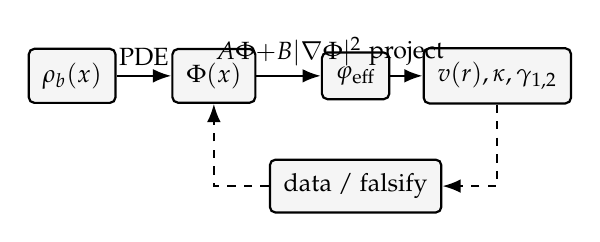
\begin{tikzpicture}[>=Latex, node distance=1.8cm,
    box/.style={draw, thick, rounded corners=2pt, fill=gray!8,
                inner sep=5pt, align=center, font=\small}]
    \node[box] (rho) {$\rho_b(x)$};
    \node[box, right of=rho] (phi) {$\Phi(x)$};
    \node[box, right of=phi] (pot) {$\varphi_{\mathrm{eff}}$};
    \node[box, right of=pot] (obs) {$v(r),\kappa,\gamma_{1,2}$};
    \node[box, below of=pot, yshift=0.4cm] (data) {\small data / falsify};
    \draw[->, thick] (rho) -- node[above, font=\small] {PDE} (phi);
    \draw[->, thick] (phi) -- node[above, font=\small] {$A\Phi{+}B|\nabla\Phi|^2$} (pot);
    \draw[->, thick] (pot) -- node[above, font=\small] {project} (obs);
    \draw[->, thick, dashed] (obs) |- (data);
    \draw[->, thick, dashed] (data) -| (phi);
\end{tikzpicture}
\caption{Forward-model pipeline for synchronization cosmology. The same field $\Phi[\rho_b]$ must reproduce both rotation curves and lensing; separate fits would destroy falsifiability.}
\end{figure}

% ============================================================
\section{Rotation-Curve Scaling from Scale-Free Synchronization}
% ============================================================

We derive the asymptotic rotation-curve law implied by the minimal
synchronization model and show that it reproduces the baryonic Tully--Fisher
relation without free parameters.

\subsection{Scale-Free Coherence Profiles}

Let the effective gravitational potential be identified with the projected
coherence field: $\varphi_{\mathrm{eff}}(r) = \Phi(r)$. For circular motion,
\[
    v_{\mathrm{rot}}^2(r)
    =
    r\,\left|\frac{d\varphi_{\mathrm{eff}}}{dr}\right|
    =
    r\,\left|\frac{d\Phi}{dr}\right|.
\]
Outside the baryonic core, the synchronization field is governed by scale-free
coherence. The only radial profile with no preferred length scale and nonzero
radial flux is logarithmic:
\[
    \Phi(r) = A\log(r/r_0),\quad
    \frac{d\Phi}{dr} = \frac{A}{r},\quad
    v_{\mathrm{rot}}^2 = A.
\]
Flat rotation curves therefore follow directly from scale-free synchronization,
with no tuning.

\subsection{The Square-Root Coherence Response}

To connect $A$ to baryonic matter, define the total baryonic source strength
$M_b = \int\rho_b\,d^3x$ and the total coherence charge $Q_\Phi$. The minimal
assumption is $Q_\Phi \propto M_b$. The amplitude $A$ of the logarithmic
coherence profile is set by the radial flux at the baryonic radius, which under
scale-free synchronization satisfies
\[
    A \sim Q_\Phi^{1/2} \propto M_b^{1/2}.
\]
The square-root exponent arises because $A$ is the amplitude of a logarithmic
potential sourced by a coherence charge, and the relationship between source
charge and field amplitude for a logarithmic potential is sub-linear. Then
\[
    v_{\mathrm{rot}}^2 = A \propto M_b^{1/2},
\]
so that
\[
    v_{\mathrm{rot}}^4 \propto M_b.
\]

\begin{proposition}[Baryonic Tully--Fisher from Scale-Free Synchronization]
Under the minimal synchronization model with logarithmic coherence profile and
linear coherence-charge response, the rotation velocity satisfies
$v_{\mathrm{rot}}^4 \propto M_b$ without a dark matter halo and without an
empirical interpolation function.
\end{proposition}

\subsection{Interpretation}

The scaling arises from two independent facts. First, scale-free synchronization
forces $d\Phi/dr \sim 1/r$, which immediately implies flat rotation curves.
Second, the amplitude $A$ satisfies a square-root response to the baryonic
source, giving the Tully--Fisher exponent. The crucial move is the square-root
coherence response: without it, the model gives flat curves but not the baryonic
scaling. Together, these two properties recover the observed relation purely from
synchronization geometry, placing the model in direct empirical competition with
both $\Lambda$CDM halo models and the MOND interpolation function $\mu(a/a_0)$.

% ============================================================
\section{Relation to Numerical Cosmology and the Illustris Pipeline}
% ============================================================

Modern cosmological understanding is strongly shaped by large-scale numerical
simulations, most notably the Illustris Project and its successor IllustrisTNG
\cite{vogelsberger2014,nelson2018}, which evolve coupled systems of dark matter,
baryonic gas, and feedback processes within the $\Lambda$CDM framework using
$N$-body gravity, finite-volume hydrodynamics, and subgrid prescriptions for
star formation. The resulting outputs reproduce large-scale structure, galaxy
populations, and statistical observables with remarkable fidelity.

The synchronization-based framework differs at a foundational level in its
choice of dynamical variables. Rather than evolving particle ensembles, the
present model evolves a continuous coherence field $\Phi(x,t)$ governed by
equation~\eqref{eq:phi_closure}. Standard simulations implement a forward
pipeline $(\rho_{\mathrm{DM}},\rho_{\mathrm{baryon}}) \to \text{particle
dynamics} \to \text{gravitational potential} \to \text{observables}$. The
synchronization framework replaces particle dynamics with field relaxation:
$\rho_{\mathrm{baryon}} \to \Phi \to \varphi_{\mathrm{eff}} \to
\text{observables}$. The dominant computational task shifts from $N$-body
integration to the solution of nonlinear elliptic PDEs, which scale with grid
resolution rather than particle number.

\begin{proposition}[Simulation Equivalence Test]
Let $\rho_b$ be a baryonic density field obtained from a $\Lambda$CDM
simulation. If there exists a parameter set for the synchronization field such
that the resulting $\varphi_{\mathrm{eff}}$ reproduces both the simulated
rotation curves and lensing maps, then the coherence framework provides an
observationally equivalent description of the gravitational dynamics.
\end{proposition}

\subsection{Benchmark Case Study: Reconstructing a Simulated Halo Without Dark Matter}

Given $\rho_b(x)$ extracted from Illustris, the standard pipeline computes
$\nabla^2\varphi_{\mathrm{tot}} = 4\pi G(\rho_b + \rho_{\mathrm{DM}})$. In
the synchronization framework, one instead solves
\begin{equation}
-\nabla\cdot(D(\Phi)\nabla\Phi)
+
\alpha\Phi^3 - \beta\Phi
=
\gamma\rho_b(x),
\label{eq:phi_halo}
\end{equation}
then defines $\varphi_{\mathrm{eff}} = \varphi_b + \lambda_1\Phi +
\lambda_2|\nabla\Phi|^2$, and computes $v_c(r) =
\sqrt{r\,d\varphi_{\mathrm{eff}}/dr}$ and $\kappa(x_\perp) \propto
\nabla_\perp^2\varphi_{\mathrm{eff}}$. The reconstruction succeeds if flat
rotation curves emerge at large radii without $\rho_{\mathrm{DM}}$, lensing
convergence maps reproduce the amplitude and spatial distribution of the
simulated signal, and the inferred $\Phi(x)$ exhibits extended structure beyond
the baryonic distribution, effectively mimicking a halo.

\begin{remark}
This procedure does not claim that dark matter is absent at a fundamental level.
Rather, it shows that its phenomenological role may be realized by an emergent
field degree of freedom. Distinguishing between these possibilities requires
observables sensitive to dynamical response, not merely static structure.
\end{remark}

% ============================================================
\section{Comparative Predictions Across Cosmological Frameworks}
% ============================================================

We compare three classes of models: $\Lambda$CDM with cold dark matter, Modified
Newtonian Dynamics (MOND) \cite{milgrom1983}, and the constrained-field
synchronization model developed here. The comparison is restricted to qualitative
structure, scaling relations, and observable dependencies.

\subsection{Rotation Curves}

In $\Lambda$CDM, flat rotation curves are produced by halo mass profiles and
the dependence on baryons is indirect via halo formation. In MOND, the
low-acceleration scaling is imposed as a fundamental relation through the
universal scale $a_0$, with low scatter predicted. In the synchronization
framework, flat curves emerge from $\Phi$ coherence coupling, the dependence
on baryons is direct through the source term in equation~\eqref{eq:phi_closure},
and low scatter emerges if $\Phi$ equilibrates with $\rho_b$.

\subsection{Gravitational Lensing}

$\Lambda$CDM sources lensing from total mass and naturally accommodates
mass-light offsets through collisionless dark matter. MOND requires a
relativistic extension for lensing and generally underpredicts cluster lensing
strength. The synchronization model sources lensing from
$\varphi_{\mathrm{eff}}[\Phi,\rho_b]$; offsets between baryonic matter and
lensing centers arise from finite relaxation time of $\Phi$, and cluster lensing
strength must arise from the extended field structure.

\subsection{Structure Formation}

$\Lambda$CDM seeds structure through dark matter seeds with a well-developed
halo mass function and filamentary cosmic web. MOND produces structure less
naturally. The synchronization model generates early growth through coupled
$\Phi$--baryon instability, filaments as $\Phi$ coherence domain boundaries,
and halo universality emerging from the PDE structure of
equation~\eqref{eq:phi_closure}.

\subsection{Dynamical Memory}

Only the synchronization framework generically predicts finite relaxation of
the gravitational response. $\Lambda$CDM shows collisionless relaxation with
no memory of prior trajectory classes. MOND is effectively instantaneous.
The synchronization model allows observable lag and hysteresis, making it the
only framework that predicts correlations between current gravitational response
and prior dynamical history.

\subsection{Discriminating Observables}

Three classes of observation can distinguish the models without parameter
fitting. Offset systems such as merging clusters distinguish $\Lambda$CDM
(persistent mass-light separation from collisionless dark matter) from MOND
(struggles without additional fields) from the $\Phi$-model (separation only
if $\Phi$ has finite relaxation time). Galaxy rotation scaling relations are
exact in MOND, emergent with scatter in $\Lambda$CDM, and emergent if $\Phi$
equilibrates in the synchronization model. Time-dependent lensing or dynamics
are absent from $\Lambda$CDM and MOND but generically predicted by the $\Phi$
model through lag between baryonic motion and effective gravitational response.

% ============================================================
\section{Observational Strategy for Detecting Field Relaxation}
% ============================================================

A distinguishing feature of the synchronization framework is that the effective
gravitational response is mediated by a dynamical field $\Phi(x,t)$ with finite
relaxation time. We outline observational strategies to detect such relaxation
using existing and near-term datasets.

\subsection{Merging Galaxy Clusters}

Merging clusters provide the cleanest test. In systems such as the Bullet
Cluster \cite{clowe2006}, X-ray observations trace collisional gas while
lensing maps the effective mass distribution. Three regimes can be
distinguished: $\Lambda$CDM predicts lensing peaks tracking collisionless dark
matter with persistent offset from baryonic gas; instantaneous modified gravity
predicts lensing closely following baryonic mass; the synchronization field
predicts lensing remaining offset from baryons temporarily if $\Phi$ has not
yet relaxed to the new baryonic configuration. A systematic survey of merging
clusters at different merger stages can therefore test for time-dependent
alignment between baryonic and lensing peaks.

\subsection{Time-Resolved Strong Lensing}

Strong lensing systems with variable sources provide a complementary probe.
If $\Phi$ evolves on observable timescales, time-delay measurements taken at
different epochs may show systematic shifts not attributable to source
variability alone, and lens models reconstructed from different epochs may
require slightly different effective potentials even when baryonic structure
appears unchanged.

\subsection{Galaxy Rotation During Transients}

Galaxies undergoing rapid baryonic reconfiguration---starbursts,
feedback-driven outflows, tidal interactions---offer a dynamical test.
Transient deviations from equilibrium rotation profiles may persist longer
than expected from baryonic evolution alone, and hysteresis effects may appear
in which the rotation curve depends on recent history rather than only current
mass distribution.

\subsection{Large-Scale Structure Evolution}

On cosmological scales, programs such as the Dark Energy Survey and the Euclid
mission measure clustering statistics, growth rates, and weak lensing shear
fields. A finite relaxation time for $\Phi$ would manifest as scale-dependent
deviations in growth rates, mild decorrelation between baryonic tracers and
lensing fields, and evolution-dependent bias between observed structure and
inferred gravitational potential.

\subsection{A No-Go Result for Instantaneous Gravitational Response}

We formalize the distinction between instantaneous and dynamical response.

\begin{definition}[Instantaneous Response Model]
A gravitational model has instantaneous response if $\varphi_{\mathrm{eff}}(x,t)
= \mathcal{G}[\rho_b(\cdot,t)](x)$ for some functional $\mathcal{G}$, with no
dependence on prior history.
\end{definition}

\begin{definition}[Dynamical Response Model]
A model has dynamical response if $\varphi_{\mathrm{eff}}$ depends on the
history $\{\rho_b(\cdot,s)\}_{s \leq t}$ with $\partial_t\mathcal{H} \neq 0$
even when $\rho_b$ is held fixed.
\end{definition}

\begin{proposition}[No Persistent Lag in Instantaneous Models]
In any instantaneous response model, two systems with identical baryonic
configurations at time $t$ must have identical effective potentials at time $t$.
Persistent lag or hysteresis correlated with evolutionary history cannot arise
without explicit additional state variables.
\end{proposition}

\begin{proof}
By definition $\varphi_{\mathrm{eff}}^{(1)}(\cdot,t) = \mathcal{G}[\rho_b^{(1)}
(\cdot,t)]$ and $\varphi_{\mathrm{eff}}^{(2)}(\cdot,t) = \mathcal{G}[\rho_b^{(2)}
(\cdot,t)]$. If $\rho_b^{(1)}(\cdot,t) = \rho_b^{(2)}(\cdot,t)$, then
$\varphi_{\mathrm{eff}}^{(1)} = \varphi_{\mathrm{eff}}^{(2)}$. Observed differences
correlated with prior trajectories are therefore inadmissible within this class.
\end{proof}

\begin{corollary}[Hysteresis as Evidence of Dynamical Fields]
If there exist systems with indistinguishable baryonic configurations at time $t$
but measurably different gravitational responses correlated with evolutionary
history, then no instantaneous response model can account for the observations.
Such behavior requires a dynamical mediating field or additional hidden degrees
of freedom.
\end{corollary}

\begin{remark}
This result does not distinguish between dark matter and dynamical-field
interpretations. It establishes only that any theory reproducing persistent
lag must include additional state variables beyond the instantaneous baryonic
configuration. In $\Lambda$CDM these are collisionless matter components; in
the present framework they are encoded in the evolving field $\Phi$.
In this sense, gravitational dynamics can be tested for Markovianity.
\end{remark}

\begin{figure}[ht]
\centering
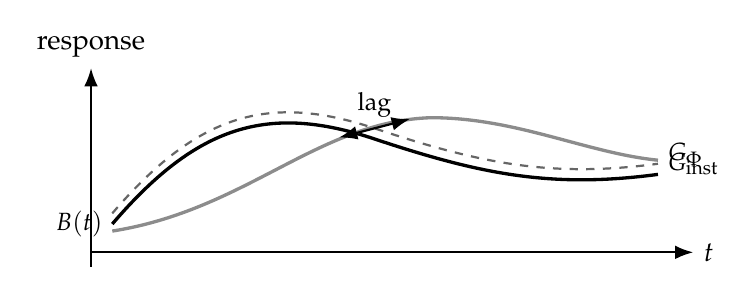
\begin{tikzpicture}[scale=0.9, >=Latex]
    \draw[->, thick] (0,0) -- (8.5,0) node[right] {$t$};
    \draw[->, thick] (0,-0.2) -- (0,2.6) node[above] {response};
    % baryonic tracer B(t)
    \draw[very thick]
        (0.3,0.4) .. controls (1.5,1.8) and (2.5,2.1) ..
        (4.0,1.6) .. controls (5.5,1.1) and (6.5,0.9) .. (8.0,1.1);
    \node[left, font=\small] at (0.3,0.4) {$B(t)$};
    % instantaneous response G_inst (traces B exactly, offset up slightly)
    \draw[thick, dashed, black!60]
        (0.3,0.55) .. controls (1.5,1.95) and (2.5,2.25) ..
        (4.0,1.75) .. controls (5.5,1.25) and (6.5,1.05) .. (8.0,1.25);
    \node[right, font=\small] at (8.0,1.25) {$G_{\mathrm{inst}}$};
    % delayed response G_Phi (lags and is smoothed)
    \draw[very thick, black!45]
        (0.3,0.3) .. controls (2.2,0.6) and (3.2,1.85) ..
        (4.8,1.9) .. controls (6.0,1.9) and (7.0,1.4) .. (8.0,1.3);
    \node[right, font=\small] at (8.0,1.3) {\raisebox{6pt}{$G_{\Phi}$}};
    % lag arrow
    \draw[<->, thick] (3.5,1.62) -- (4.5,1.88)
        node[midway, above, font=\small] {lag};
\end{tikzpicture}
\caption{Instantaneous response $G_{\mathrm{inst}}$ tracks the baryonic tracer $B(t)$ exactly; the dynamical $\Phi$-field response $G_\Phi$ exhibits finite lag. The no-go proposition shows this distinction is structurally unavoidable.}
\end{figure}

\subsection{Falsification Protocol}

The following protocol operationalizes the no-go result without assuming a
specific model. For each system $k$ at epoch $t$, measure a baryonic tracer
$B_k(x,t)$ (stellar light or gas density) and a gravitational proxy $G_k(x,t)$
(lensing convergence or kinematic potential). Construct pairs $(k,\ell)$ with
$\|B_k(\cdot,t) - B_\ell(\cdot,t)\| \leq \varepsilon$ for an observational
tolerance $\varepsilon$. Define the gravitational mismatch $\Delta_{k\ell} :=
\|G_k(\cdot,t) - G_\ell(\cdot,t)\|$. Evaluate whether $\Delta_{k\ell}$ exhibits
systematic dependence on independent indicators of recent evolution (merger
stage, starburst activity, gas disturbance) after controlling for redshift,
environment, and resolution.

If $\Delta_{k\ell} \approx 0$ for all matched pairs, results are consistent
with instantaneous response. If $\Delta_{k\ell}$ is nonzero and correlates
with indicators of past dynamical activity, this constitutes evidence of
history dependence in the gravitational response. The protocol probes a
structural property---memory versus instantaneity---and is therefore
model-independent at the level of hypothesis testing.

% ============================================================
\section{Limitations and Open Problems}
% ============================================================

The framework presented here is intentionally minimal and operates at the level
of effective field theory. Several significant limitations and open problems
remain across the four layers of the paper.

\paragraph{Effective field description.}
The fields $\Phi$, $\mathbf{v}$, and $\Sfield$ are coarse-grained effective
variables and do not uniquely determine microscopic configurations. The
derivation of the free-energy functional $\F$ from a specific microscopic model
remains open for most systems of interest. Similarly, the memory operators
$\mathcal{K}_\Phi$, $\mathcal{K}_{\mathbf{v}}$, $\mathcal{K}_{\Sfield}$
introduced in Section~8 are phenomenological; their rigorous derivation from
projection operator methods or memory function formalisms would substantially
strengthen the framework.

\paragraph{Accessibility collapse and calibration.}
The term $-\beta(\Phi)\Sfield$ in equation~\eqref{eq:S_evo} is the most
mechanically novel element of the framework. Its quantitative calibration
against experimental relaxation data has not been performed, and the functional
form of $\beta(\Phi)$ is taken as monotone increasing without further
specification. Whether $\beta$ depends on additional fields, on the history
$\mathcal{M}$, or on spatial gradients of $\Phi$ is an open question whose
answer would determine whether the collapse dynamics belong to a known
universality class.

\paragraph{Derived sheaf truncation.}
Section~12 treats the configuration sheaf as a 1-sheaf in the low-accessibility
regime and notes that the high-accessibility regime requires a derived stack
with nontrivial higher gluing data. The precise conditions under which the
truncation from a derived sheaf to a 1-sheaf is valid, the nature of the higher
morphisms encoding trajectory memory, and the connection to existing derived
algebraic geometry remain to be developed. In particular, the relationship
between the memory kernels $\mathcal{M}_i$ and the $(\infty,1)$-categorical
structure of $\mathcal{C}_{\mathrm{adm}}$ requires rigorous treatment.

\paragraph{Reconstruction and inverse problems.}
The reconstruction of $\X$ from experimental projections $\{\Pi_k[\X]\}$ is
an ill-posed inverse problem in general. The forward model is well-defined, but
the regularization required for stable inversion---particularly in the presence
of higher sheaf obstructions---is not specified. The admissibility log simulator
described in Appendix~A provides a forward model but not an inversion scheme.

\paragraph{Cosmological coupling and lensing constraints.}
The closure relation $\Delta\Phi - m^2\Phi + \lambda\Phi^3 = \alpha\rho_b +
\gamma|\nabla\Phi|^2$ contains six free parameters $\{A,B,\alpha,m^2,\lambda,
\gamma\}$ that must be fit simultaneously to rotation curves and lensing
observables. No such fit has been performed. In particular, the simultaneous
reproduction of weak lensing shear correlations and the cluster-scale lensing
convergence --- the hardest constraint from the Bullet Cluster geometry --- has
not been demonstrated. Failure on this constraint would falsify the closure
relation as stated and require a modified coupling between $\Phi$ and the
effective metric.

\paragraph{Relativistic consistency at strong curvature.}
The derivation of the effective metric in Section~17 operates in the weak-field
perturbative regime. Whether the synchronization framework extends consistently
to strong-field regimes --- compact objects, black holes, gravitational wave
generation --- has not been examined. The stress-energy tensor
$T_{\mu\nu}^{\Phi,\mathbf{v},\Sfield}$ appearing in the modified Einstein
equations is not fully specified, and its positivity properties (required for
energy conditions) are not verified.

\paragraph{Recency optimality beyond exponential decay.}
The recency optimality proposition of Section~21 is proved under an exponential
decay condition on constraint evolution. Whether power-law decay or other
non-exponential memory structures --- which arise in systems exhibiting
scale-free dynamics or long-range correlation --- can be handled within the same
framework requires extension of the result. The relationship between the memory
kernel $K_i(t-s)$ of Section~7 and the optimal truncation of the admissibility
log is not worked out in general.

\paragraph{Socio-technical calibration.}
The modular externalization section of Section~20 provides a formal structure
but no quantitative predictions. The conditions under which admissible residues
generate genuinely new trajectory classes, as opposed to merely expanding the
volume within existing classes, require a theory of combinatorial accessibility
growth that is not developed here.

These limitations define the frontier of the framework. The most
decision-critical open problem for the paper's primary claims is the
cosmological lensing constraint: simultaneous fit of rotation curves and lensing
from a single $\Phi[\rho_b]$ without dark matter is the make-or-break test for
the synchronization extension.

% ============================================================
\section{Conclusion: From Structure to Constrained Trajectories}
% ============================================================

We have argued that mesoscale systems across soft matter physics, biophysics,
nanotechnology, and materials engineering share a common mathematical structure.
By representing these systems through a coupled field
$\X(x,t) = (\Phi, \mathbf{v}, \Sfield)$, we obtain a unified description in
which structure, transport, and configurational accessibility are intrinsically
linked.

Within this framework, self-assembly is reinterpreted as constrained exploration
of configuration space. Structure emerges as a field encoding correlations and
admissibility, while transport arises as motion constrained by this field and
feeds back into it through the coupling term $\mu'(\Phi)|\mathbf{v}|^2$.
Interfaces act as active boundaries whose stability arises from the local
suppression of configurational accessibility. Dynamics are understood as
trajectories through configuration space, and functional behavior corresponds
to the stabilization of those trajectories in low-$\Sfield$ basins.

The introduction of trajectory-aware representation extends this picture by
incorporating non-Markovian memory and cross-scale consistency. Systems are no
longer described solely by their instantaneous configurations, but by overlapping
patches of reconstructible trajectories. The Wilson façade structure provides
the conceptual foundation for this move: the patchwork of locally valid
descriptions, with handoff conditions at the seams, is not an approximation of
a hidden global theory but the operative structure of physical description
itself.

The configurational accessibility field $\Sfield$ provides the central unifying
quantity. It measures the local density of admissible trajectories and governs
both the exploration and restriction of configuration space. The term
$-\lambda\Sfield$ in the free-energy functional drives the system toward
configurations with many admissible futures, while the dynamical term
$-\beta(\Phi)\Sfield$ encodes the irreversible collapse of accessibility
induced by increasing constraint. The competition between these two tendencies
governs the transient accessibility landscape and determines which regions of
configuration space remain reachable. In particular, regions that transiently
increase in $\Phi$ experience accelerated accessibility collapse, making such
fluctuations self-reinforcing and driving the system toward locally irreversible
organization.

This geometric picture admits a natural topological refinement. As constraints
accumulate, not only does the volume of accessible trajectories decrease, but
the number of admissible homotopy classes contracts. Structured evolution
therefore corresponds to a joint reduction in geometric accessibility and
topological diversity. Novelty corresponds to structured accessibility
reduction; compression corresponds to the elimination of entire classes of
trajectories. Functional systems arise when this process stabilizes: trajectories
become confined to a small number of homotopy classes, and perturbations no
longer induce transitions between them.

\begin{quote}
Function corresponds to confinement within a restricted set of admissible
trajectory classes.
\end{quote}

From this perspective, design can be interpreted as the controlled induction of
accessibility collapse along targeted trajectories: not the imposition of
structure directly, but the progressive removal of alternative futures until
only the desired evolution remains dynamically admissible. Processes such as
cross-linking, crystallization, alignment, and templating are mechanisms for
inducing this collapse in targeted regions of configuration space. Biological
systems achieve similar effects through sequence-encoded folding pathways and
cooperative assembly.

Mesoscale matter is therefore not defined by what it is, but by how it evolves
under constraint. Structure, transport, and function are different expressions
of the same underlying process: the structured collapse of possibility space.
Geometry emerges as the minimal global structure required to represent a sheaf
of admissible configurations once higher cohomological obstructions have
vanished.

\bigskip

\noindent\textit{Mesoscale systems are not merely structured---they are
structured in motion. Understanding them requires tracing the constrained
trajectories through which configurations emerge, and identifying the
accessibility and homotopy collapse that render those trajectories stable
enough to be called functional.}

\newpage

\appendix
{\small

% ============================================================
\section{Algorithms for the Admissibility Log Simulator}
% ============================================================

This appendix describes three algorithms that implement the admissibility log
as an executable object, grounding the formal constructions of Sections~8
and~9 in a concrete computational procedure. The algorithms are presented as
structured pseudocode; an Abraxas-compatible numerical implementation follows
the same structure directly.

\subsection{Algorithm 1: RSVP Field Initialization and Event Application}

The system state is a tuple $(\Phi, \mathbf{v}, \Sfield, R)$ defined on a
discrete spatial grid of width $W$ and height $H$, where $R$ denotes the
residue field accumulating gluing obstruction. Fields are initialized as
$\Phi = 0$, $\mathbf{v} = 0$, $\Sfield = \Sfield_0$ for a baseline
accessibility $\Sfield_0 \in (0,1)$, and $R = 0$.

A discrete event $e = (x,y,\Delta\Phi,\Delta\mathbf{v},\Delta\Sfield)$
is applied by a Gaussian kernel of width $\sigma$:
\[
    w_{ij} = \exp\!\left(-\frac{(i-y)^2 + (j-x)^2}{\sigma^2}\right).
\]
Each field component is updated pointwise:
$\Phi_{ij} \leftarrow \Phi_{ij} + w_{ij}\Delta\Phi$, and similarly for
$\mathbf{v}$ and $\Sfield$. The residue field accumulates the magnitude of
the structural update: $R_{ij} \leftarrow R_{ij} + |w_{ij}\Delta\Phi|\,\rho$
for a residue coupling $\rho > 0$. The Gaussian smearing ensures that discrete
events approximate localized field operators, so that the continuum limit
$\Delta t \to 0$ recovers the RSVP evolution equations.

\subsection{Algorithm 2: RSVP Relaxation Step}

Between events, the field evolves by a single relaxation step that approximates
the coupled PDE dynamics. Spatial gradients of $\Phi$ are estimated by
finite differences:
\[
    (\nabla\Phi)_x \approx \frac{\Phi_{i,j+1} - \Phi_{i,j-1}}{2},
    \qquad
    (\nabla\Phi)_y \approx \frac{\Phi_{i+1,j} - \Phi_{i-1,j}}{2},
\]
using periodic boundary conditions. The transport field is updated by gradient
alignment:
$\mathbf{v} \leftarrow \mathbf{v} + \alpha_v \nabla\Phi$, implementing the
admissible flux condition that transport follows structural constraint gradients.

The accessibility field evolves by the collapse equation: the effective
collapse rate $\beta_{ij} = \beta_0 + \beta_1\,\max(\Phi_{ij},0)$ encodes the
state-dependent feedback $\beta'(\Phi) > 0$, so that ordered regions suppress
accessibility faster. The update is
$\Sfield_{ij} \leftarrow \Sfield_{ij} + \alpha_\Phi |\mathbf{v}_{ij}|^2 -
\beta_{ij}\Sfield_{ij}$, where the first term is transport-induced
diversification and the second is constraint-induced collapse.

The structural field diffuses by a discrete Laplacian:
$\Phi \leftarrow (1-\epsilon)\Phi + \epsilon \,\bar\Phi$, where $\bar\Phi$
denotes the local spatial average. This implements the coarse-graining pushforward
$\pi_*\mathcal{F}$ at the level of the scalar field. Field values are clipped to
$[-1,1]$ for $\Phi$ and $[0,1]$ for $\Sfield$.

\subsection{Algorithm 3: Gluing Obstruction Estimation}

The sheaf gluing obstruction is estimated by a patch-based mismatch computation.
The spatial domain is covered by overlapping square patches of side length $\ell$
with stride $s < \ell$, so that neighboring patches overlap in a strip of width
$\ell - s$. For each patch, the local mean $\bar\Phi_{\mathrm{patch}}$ is
computed. The local gluing mismatch at each grid point is
\[
    \delta_{ij}
    =
    |\Phi_{ij} - \bar\Phi_{\mathrm{patch}(i,j)}|,
\]
where $\mathrm{patch}(i,j)$ denotes the patch containing grid point $(i,j)$.
Multiple overlapping patches contribute independently, and contributions are
averaged. The result is added to the residue field:
$R_{ij} \leftarrow R_{ij} + \mu\,\delta_{ij}$, where $\mu > 0$ is a gluing
weight. A large $R$ at a grid point indicates high local inconsistency between
patches, corresponding to a nontrivial \v{C}ech cochain
$[\delta] \in \check{H}^1(\{U_i\},\mathcal{F})$.

\subsection{Visualization Interpretation}

The output of a simulation run is a sequence of frames, each containing the
current values of $\Phi$, $\mathbf{v}$, $\Sfield$, and $R$. A natural
color encoding assigns the red channel to the gluing residue $R$ (obstruction
intensity), the green channel to structural order $\Phi$ (shifted to $[0,1]$),
and the blue channel to configurational accessibility $\Sfield$. In this
encoding, regions of high structural order and low accessibility appear green
with suppressed blue, corresponding to functional lock-in; regions of high
residue and disordered structure appear red, corresponding to gluing failure;
and regions of balanced accessibility appear with prominent blue, corresponding
to exploratory dynamics. The vector field $\mathbf{v}$ may be overlaid as a
flow visualization to show transport pathways and their alignment with
structural constraint gradients.

% ============================================================
\section{Algorithm for the Cosmological Synchronization Forward Model}
% ============================================================

This appendix section describes the numerical procedure for the cosmological
synchronization forward model of Section~24. The algorithm maps a baryonic
density field to effective gravitational observables via the synchronization
field $\Phi$, without invoking dark matter as an explicit particle component.

\subsection{Algorithm 4: Synchronization Field Solver}

Input: a baryonic density field $\rho_b(x)$ on a three-dimensional grid of
spacing $h$. Parameters: coherence decay scale $m^{-1}$, baryonic coupling
$\alpha$, saturation coefficient $\lambda$, gradient reinforcement $\gamma$,
relaxation step $\eta$, convergence tolerance $\delta_{\mathrm{tol}}$.

Initialize $\Phi^{(0)} = 0$ on the grid. At each iteration $n$, compute the
discrete Laplacian $\Delta\Phi^{(n)}$ by finite differences with periodic or
zero boundary conditions, and the squared gradient magnitude $|\nabla\Phi^{(n)}|^2$
from centered differences. The residual is
\[
r^{(n)}
=
\Delta\Phi^{(n)} - m^2\Phi^{(n)} + \lambda(\Phi^{(n)})^3
- \alpha\rho_b - \gamma|\nabla\Phi^{(n)}|^2.
\]
Update $\Phi^{(n+1)} = \Phi^{(n)} + \eta\,r^{(n)}$. Clip values to a
physically admissible range $[-\Phi_{\max},\Phi_{\max}]$. Iterate until
$\|r^{(n)}\|_\infty < \delta_{\mathrm{tol}}$.

\subsection{Algorithm 5: Effective Potential and Observable Construction}

Given a converged field $\Phi(x)$:

Compute the effective gravitational potential
$\varphi_{\mathrm{eff}} = A\Phi + B|\nabla\Phi|^2$.

For rotation curves: extract a radial profile $\varphi_{\mathrm{eff}}(r)$
from the cylindrically averaged potential and compute $v_c(r) =
\sqrt{r\,d\varphi_{\mathrm{eff}}/dr}$ by numerical differentiation.

For lensing: project the potential along the line of sight to obtain
$\psi_{\mathrm{lens}}(x_\perp) = (2/c^2)\int\varphi_{\mathrm{eff}}\,dz$.
Then compute convergence $\kappa = \frac{1}{2}\nabla_\perp^2\psi_{\mathrm{lens}}$
and shear components $\gamma_1 = \frac{1}{2}(\partial_{x}^2 -
\partial_{y}^2)\psi_{\mathrm{lens}}$ and $\gamma_2 =
\partial_x\partial_y\psi_{\mathrm{lens}}$ by finite differences on the
projected grid.

For the effective dark matter analog: define $\rho_{\mathrm{eff}} =
(4\pi G)^{-1}\Delta\varphi_{\mathrm{eff}}$ and compare its spatial distribution
to the dark matter halo inferred from the standard simulation. Agreement
indicates that the coherence field reproduces the gravitational role of dark
matter from baryonic sources alone.

\subsection{Calibration and Falsification Criterion}

Fit the six parameters $\{A, B, \alpha, m^2, \lambda, \gamma\}$ to a training
set of galaxies with measured rotation curves and lensing profiles. The model
is validated only if a single parameter set simultaneously reproduces rotation,
weak lensing shear, and cluster convergence maps across independent test systems.
Failure on any one observable class falsifies the closure relation
equation~\eqref{eq:phi_closure}. The strongest test is the Bullet Cluster
geometry \cite{clowe2006}: the forward model must produce a lensing centroid
offset from the baryonic X-ray centroid without invoking collisionless particles.

% ============================================================
\section{BNF Specification for the Synchronization-Field Simulator}
% ============================================================

This appendix gives a formal grammar for specifying numerical simulations of
the five-dimensional Ising synchronization model. The grammar is written in
Backus--Naur form and defines a compact configuration language for simulations
of $\sigma : \mathbb{R}^3 \times \mathbb{R} \times \Xi \to \{-1,+1\}$.

\subsection{Grammar}

{\footnotesize\begin{verbatim}
<simulation>  ::= "simulation" <id> "{" <body> "}"
<body>        ::= <domain> | <field> | <initialization>
               | <dynamics> | <projection>
               | <observables> | <output> | <body> <body>
<domain>      ::= "domain" "{" "space" "=" <grid3> ";"
                  "time" "=" <timegrid> ";"
                  "internal" "=" <internalgrid> ";"
                  "boundary" "=" <boundary> ";" "}"
<grid3>       ::= "(" <int> "," <int> "," <int> ")"
<timegrid>    ::= "(" <real> "," <real> "," <real> ")"
<internalgrid>::= "(" <int> ")"
<boundary>    ::= "periodic" | "reflecting" | "open"
<field>       ::= "field" "{" "sigma" ":" "ising5d" ";"
                  "phi" ":" "projection" ";"
                  "v" ":" "gradient" ";"
                  "S" ":" "accessibility" ";" "}"
<init>        ::= "initialize" "{" "sigma" "=" <initrule> ";"
                  "seed" "=" <int> ";" "}"
<initrule>    ::= "random" | "biased" "(" <real> ")"
               | "baryon_seeded" "(" <id> ")"
               | "domain_seeded" "(" <int> ")"
<dynamics>    ::= "dynamics" "{" "update" "=" <rule> ";"
                  "steps" "=" <int> ";"
                  "relaxation" "=" <real> ";" "}"
<rule>        ::= "majority" | "metropolis"
               | "heatbath" | "deterministic_sync"
<projection>  ::= "projection" "{"
                  "phi" "=" "mean_internal(sigma)" ";"
                  "v" "=" "negative_gradient(phi)" ";"
                  "S" "=" "log_variance_internal(sigma)" ";" "}"
<observables> ::= "observables" "{" <obs_list> "}"
<obs_list>    ::= <obs> | <obs> <obs_list>
<obs>         ::= "rotation_curve" ";"
               | "lensing_convergence" ";"
               | "coherence_length" ";"
               | "gluing_residue" ";"
<output>      ::= "output" "{" "format" "=" <fmt> ";"
                  "path" "=" <string> ";"
                  "cadence" "=" <int> ";" "}"
<fmt>         ::= "json" | "csv" | "hdf5" | "frames"
\end{verbatim}}

\subsection{Operational Semantics}

A simulation state is the tuple
$\mathcal{S}_n = (\sigma_n,\Phi_n,\mathbf{v}_n,\Sfield_n,t_n)$.
A single update step $\mathcal{S}_n \to \mathcal{S}_{n+1}$ is given by:
\begin{align*}
    \sigma_{n+1}(x,\xi) &= \operatorname{sign}\!\Bigl(\sum_{(x',\xi')\sim(x,\xi)}\sigma_n(x',\xi')\Bigr), \\
    \Phi_{n+1}(x) &= \tfrac{1}{|\Xi|}\sum_\xi \sigma_{n+1}(x,\xi), \\
    \mathbf{v}_{n+1}(x) &= -\nabla\Phi_{n+1}(x), \\
    \Sfield_{n+1}(x) &= \log\!\bigl(1 + \operatorname{Var}_\xi[\sigma_{n+1}]\bigr), \\
    t_{n+1} &= t_n + \Delta t.
\end{align*}
Execution terminates when $t_n \geq T$.

\subsection{Invariant Properties}

\begin{proposition}[Boundedness]
For all $n$, $\sigma_n \in \{-1,+1\}$ and therefore
$-1 \leq \Phi_n(x) \leq 1$.
\end{proposition}

\begin{proposition}[Monotonic Accessibility Collapse]
Under deterministic synchronization, $\Sfield_{n+1}(x) \leq \Sfield_n(x)$
except at domain boundaries.
\end{proposition}

\begin{proposition}[Energy Descent]
Define the discrete energy $E_n = -\sum_{\langle i,j\rangle}\sigma_i\sigma_j$.
Then $E_{n+1} \leq E_n$.
\end{proposition}

\subsection{Observable Extraction Pipeline}

Rotation curves are computed from the cylindrically averaged potential:
$v_{\mathrm{rot}}(r) = \sqrt{r\,|d\Phi/dr|}$.
The effective density analogue is $\rho_{\mathrm{eff}}(x) = -\Delta\Phi(x)$.
Lensing convergence is $\kappa(x_\perp) \propto \int\Delta_\perp\Phi\,dz$.
The coherence length is $\xi_c = \int r\,C(r)\,dr$ where
$C(r) = \langle\Phi(x)\Phi(x+r)\rangle$.

\subsection{Computational Complexity}

For grid size $N^3$ and internal dimension $M$, the update cost per step is
$\mathcal{O}(N^3 M)$, gradient computation is $\mathcal{O}(N^3)$, and total
runtime is $\mathcal{O}(T N^3 M)$. This scaling is linear in the internal
dimension, making high-dimensional synchronization computationally tractable
on modern GPU hardware.

% ============================================================
\section{Reference Implementation of the Synchronization Model}
% ============================================================

\subsection{Data Layout}

We discretize space as a cubic lattice of size $N^3$ with internal dimension
$M$. The primary state is $\sigma \in \{-1,+1\}^{N\times N\times N\times M}$,
stored as a flattened array with row-major indexing
$\texttt{idx} = (((x\cdot N + y)\cdot N + z)\cdot M + \xi)$, ensuring
coalesced memory access along the internal dimension. Derived fields
$\Phi \in \mathbb{R}^{N^3}$, $\mathbf{v} \in \mathbb{R}^{N^3\times 3}$, and
$\Sfield \in \mathbb{R}^{N^3}$ are computed from $\sigma$ at each step.

\subsection{Parallel Update Kernel}

Each thread updates one site $(x,y,z,\xi)$ by majority vote over all neighbors
in the 3D spatial stencil and both internal neighbors:
\begin{align*}
&\texttt{sum} = \sum_{(dx,dy,dz)\in\{{\pm 1, 0\}}^3\setminus\{0\}} \sigma[x{+}dx,y{+}dy,z{+}dz,\xi] \\
&\qquad +\, \sigma[x,y,z,\xi{+}1] + \sigma[x,y,z,\xi{-}1], \\
&\sigma_{\mathrm{new}}[x,y,z,\xi] = \operatorname{sign}(\texttt{sum}).
\end{align*}

\subsection{Projection Kernels}

The three derived fields are computed from $\sigma$ by independent parallel
reductions. The mean over $\xi$ gives $\Phi$; centered finite differences give
$\mathbf{v} = -\nabla\Phi$; and the log-variance over $\xi$ gives $\Sfield$.
The effective potential is computed as $\varphi_{\mathrm{eff}} = \Phi$ in the
minimal model, or $\varphi_{\mathrm{eff}} = A\Phi + B|\nabla\Phi|^2$ in the
full closure model. Rotation curves follow from radial differentiation of the
cylindrically averaged $\varphi_{\mathrm{eff}}$, and lensing convergence from
line-of-sight projection and transverse Laplacian.

% ============================================================
\section{Continuum Limit of the Synchronization Dynamics}
% ============================================================

\subsection{Coarse-Graining}

Define the coarse-grained field
$\Phi(x,t) = (1/M)\sum_\xi\sigma(x,t,\xi)$
and assume local spatial averaging over scale $\epsilon$:
$\Phi_\epsilon(x) = \int K_\epsilon(x-y)\Phi(y)\,dy$.

\subsection{Expansion of the Update Rule}

The discrete synchronization update
$\sigma^{n+1} = \operatorname{sign}(\sum_{\text{nbrs}}\sigma^n)$
can be approximated as $\sigma^{n+1} \approx \tanh(\beta\Delta\sigma^n)$.
Expanding for small gradients and projecting onto the mean field gives:

\begin{theorem}[Continuum Limit]
The discrete synchronization model converges, under coarse-graining, to a
reaction--diffusion system of Ginzburg--Landau type:
\[
    \partial_t \Phi = D\Delta\Phi - \lambda\Phi^3 + \eta,
\]
with coupled transport $\mathbf{v} = -\nabla\Phi$ and accessibility
$\partial_t\Sfield = -\alpha\Phi^2$.
\end{theorem}

\begin{proof}[Sketch]
Averaging $\tanh(\beta\Delta\sigma^n)$ over the internal dimension and
expanding $\tanh$ to cubic order yields $\partial_t\Phi \approx
D\Delta\Phi - \lambda\Phi^3 + \eta$, where $D$ and $\lambda$ are determined
by the lattice geometry and $\eta$ encodes residual fluctuations. The
accessibility equation follows from $\partial_t\operatorname{Var}_\xi[\sigma]
\propto -\Phi^2$ under majority-vote dynamics.
\end{proof}

\subsection{Emergence of Effective Gravity}

Setting $\varphi = \Phi$ and taking the equilibrium limit $\partial_t\Phi = 0$
with $\lambda\Phi^3 \ll D\Delta\Phi$ gives $D\Delta\Phi \approx
-\gamma\rho_b$, recovering a Poisson-like equation
$\nabla^2\varphi = \rho_{\mathrm{eff}}$. The effective density
$\rho_{\mathrm{eff}} = -D^{-1}\gamma\rho_b$ is proportional to baryonic
matter, so standard gravitational behavior is recovered in the high-density
limit. Deviations arise in the low-density regime where the cubic term
$\lambda\Phi^3$ becomes negligible and coherence extends beyond baryonic
support, generating the additional effective potential responsible for flat
rotation curves and extended lensing.

\newpage

\begin{thebibliography}{99}

\bibitem{peng2011}
S.~Peng, Q.~Guo, T.~C.~Hughes, and P.~G.~Hartley,
\newblock In situ synchrotron SAXS study of polymerizable microemulsions,
\newblock \emph{Macromolecules} \textbf{44}, 3007--3015 (2011).

\bibitem{weigt2011}
K.~M.~Weigandt, L.~Porcar, and D.~C.~Pozzo,
\newblock In situ neutron scattering study of structural transitions in fibrin
networks under shear deformation,
\newblock \emph{Soft Matter} \textbf{7}, 9992 (2011).

\bibitem{newbloom2011}
G.~M.~Newbloom, F.~S.~Kim, S.~A.~Jenekhe, and D.~C.~Pozzo,
\newblock Mesoscale morphology and charge transport in colloidal networks of
poly(3-hexylthiophene),
\newblock \emph{Macromolecules} \textbf{44}, 3801--3809 (2011).

\bibitem{afifi2011}
H.~Afifi, G.~Karlsson, R.~K.~Heenan, and C.~A.~Dreiss,
\newblock Wormlike micelles with elliptical cross-section in cholesterol-based
surfactants,
\newblock \emph{Langmuir} \textbf{27}, 7480--7492 (2011).

\bibitem{pai2011}
S.~S.~Pai et al.,
\newblock Conformation of PEG chains in mono-PEGylated proteins,
\newblock \emph{Bioconjugate Chemistry} \textbf{22}, 2317--2323 (2011).

\bibitem{ossowski2012}
S.~Ossowski et al.,
\newblock Aggregation behavior of bovine $\kappa$- and $\beta$-casein,
\newblock \emph{Langmuir} \textbf{28}, 13577--13589 (2012).

\bibitem{liu2012}
L.~Liu et al.,
\newblock Conversion of concentration gradients into mechanical force via
core--shell capsules,
\newblock \emph{J.\ Phys.\ Chem.\ B} \textbf{116}, 974--979 (2012).

\bibitem{newbloom2012}
G.~M.~Newbloom, K.~M.~Weigandt, and D.~C.~Pozzo,
\newblock Structure and property development of poly(3-hexylthiophene) organogels,
\newblock \emph{Soft Matter} \textbf{8}, 8854 (2012).

\bibitem{bhat2012}
S.~N.~Bhat, R.~Di~Pietro, and H.~Sirringhaus,
\newblock Electroluminescence in ion-gel gated conjugated polymer transistors,
\newblock \emph{Chem.\ Mater.} \textbf{24}, 4060--4067 (2012).

\bibitem{larson2012}
K.~Larson-Smith and D.~C.~Pozzo,
\newblock Pickering emulsions stabilized by nanoparticle surfactants,
\newblock \emph{Langmuir} \textbf{28}, 11725--11732 (2012).

\bibitem{sirohi2026}
P.~Sirohi et al.,
\newblock PEG-like block copolymers self-assemble into stealth nanocarriers,
\newblock \emph{Advanced Science} \textbf{13}, e17048 (2026).

\bibitem{yin2026}
B.~Yin et al.,
\newblock Chlorination-controlled aggregation enabling high-efficiency organic
solar cells,
\newblock \emph{Nat.\ Commun.} \textbf{17}, 2340 (2026).

\bibitem{tancredi2026}
M.~Tancredi et al.,
\newblock Structure, flow, and functionality in rhamnolipid systems,
\newblock \emph{ACS Sustainable Chem.\ Eng.} \textbf{14}, 415--427 (2026).

\bibitem{ye2026}
Z.~Ye et al.,
\newblock Interfacial organization of nanoparticles in oil--water systems,
\newblock \emph{Food Hydrocolloids} \textbf{173}, 112255 (2026).

\bibitem{poliukhina2026}
E.~Poliukhina et al.,
\newblock Direct measurement of protein interaction potentials,
\newblock \emph{ACS Nano} \textbf{20}, 8487--8497 (2026).

\bibitem{villano2026}
E.~Villano et al.,
\newblock Microfluidic production of lipid-polymer nanoparticles for siRNA
delivery,
\newblock \emph{Int.\ J.\ Pharmaceutics} \textbf{688}, 126440 (2026).

\bibitem{agarwal2026}
M.~Agarwal, R.~Schweins, and F.~Gr\"ohn,
\newblock Light-induced structural evolution in electrostatic nanoassemblies,
\newblock \emph{Polymers} \textbf{18}, 190 (2026).

\bibitem{perez2026}
L.~Perez-Chirinos et al.,
\newblock Peptide electrostatic modulation of neural cell fate,
\newblock \emph{Advanced Science} \textbf{13}, e07946 (2026).

\bibitem{qian2026}
S.~Qian et al.,
\newblock Nanoplastic interactions with biomembranes,
\newblock \emph{Environ.\ Sci.: Nano} (2026).

\bibitem{xu2026}
Y.~Xu et al.,
\newblock Shear-induced alignment and transport in conjugated polymers,
\newblock \emph{Advanced Materials} \textbf{38}, e21831 (2026).

\bibitem{akepati2026}
S.~V.~R.~Akepati et al.,
\newblock Machine-learning analysis of 2D SAXS profiles,
\newblock \emph{ACS Meas.\ Sci.\ Au} \textbf{6}, 1--20 (2026).

\bibitem{wong2026}
J.~Wong, J.~Brousseau, and H.~M.~Titi,
\newblock Liquid crystal structure revealed by small-angle scattering,
\newblock \emph{Small Methods} \textbf{10}, e01808 (2026).

\bibitem{vitale2026}
F.~Vitale et al.,
\newblock SAXS analysis of phase transitions in surfactant systems,
\newblock \emph{J.\ Colloid Interface Sci.} \textbf{702}, 138966 (2026).

\bibitem{truong2026}
K.~Q.~K.~Truong and A.~G.~Marangoni,
\newblock Multi-scale triglyceride crystal network analysis via USAXS,
\newblock \emph{RSC Adv.} \textbf{16}, 12502--12510 (2026).

\bibitem{schmidhuber1991}
J.~Schmidhuber,
\newblock A possibility for implementing curiosity and boredom in model-building
neural controllers,
\newblock \emph{Proc.\ SAB} (1991).

\bibitem{schmidhuber2006}
J.~Schmidhuber,
\newblock Developmental robotics, optimal artificial curiosity, creativity,
music, and the fine arts,
\newblock \emph{Connection Science} \textbf{18}, 173--187 (2006).

\bibitem{wilson2006}
M.~Wilson,
\newblock \textit{Wandering Significance: An Essay on Conceptual Behaviour},
\newblock Oxford University Press, Oxford (2006).

\bibitem{wilson2017}
M.~Wilson,
\newblock \textit{Physics Avoidance: Essays in Conceptual Strategy},
\newblock Princeton University Press, Princeton (2017).

\bibitem{hamley2023}
I.~W.~Hamley,
\newblock Small angle X-ray scattering of peptides and proteins,
\newblock \emph{Chem.\ Soc.\ Rev.} \textbf{52}, 4173--4203 (2023).

\bibitem{gao2017}
J.~Gao et al.,
\newblock Controlling self-assembling peptide hydrogel properties through
network topology,
\newblock \emph{Biomacromolecules} \textbf{18}, 826--834 (2017).

\bibitem{vogelsberger2014}
M.~Vogelsberger et al.,
\newblock Introducing the Illustris Project: Simulating the coevolution of dark
and visible matter,
\newblock \emph{Mon.\ Not.\ R.\ Astron.\ Soc.} \textbf{444}, 1518--1547 (2014).

\bibitem{nelson2018}
D.~Nelson et al.,
\newblock The IllustrisTNG simulations: Public data release,
\newblock \emph{Mon.\ Not.\ R.\ Astron.\ Soc.} \textbf{475}, 624--647 (2018).

\bibitem{planck2020}
Planck Collaboration,
\newblock Planck 2018 results. VI. Cosmological parameters,
\newblock \emph{Astron.\ Astrophys.} \textbf{641}, A6 (2020).

\bibitem{milgrom1983}
M.~Milgrom,
\newblock A modification of the Newtonian dynamics as a possible alternative to
the hidden mass hypothesis,
\newblock \emph{Astrophys.\ J.} \textbf{270}, 365--370 (1983).

\bibitem{clowe2006}
D.~Clowe et al.,
\newblock A direct empirical proof of the existence of dark matter,
\newblock \emph{Astrophys.\ J.\ Lett.} \textbf{648}, L109--L113 (2006).

\bibitem{rubin1980}
V.~C.~Rubin, W.~K.~Ford Jr., and N.~Thonnard,
\newblock Rotational properties of 21 SC galaxies with a large range of
luminosities,
\newblock \emph{Astrophys.\ J.} \textbf{238}, 471--487 (1980).

\bibitem{verlinde2017}
E.~Verlinde,
\newblock Emergent gravity and the dark universe,
\newblock \emph{SciPost Physics} \textbf{2}, 016 (2017).

\bibitem{famaey2012}
B.~Famaey and S.~McGaugh,
\newblock Modified Newtonian Dynamics (MOND): Observational phenomenology and
relativistic extensions,
\newblock \emph{Living Reviews in Relativity} \textbf{15}, 10 (2012).

\bibitem{mcgaugh2016}
S.~S.~McGaugh, F.~Lelli, and J.~M.~Schombert,
\newblock Radial acceleration relation in rotationally supported galaxies,
\newblock \emph{Phys.\ Rev.\ Lett.} \textbf{117}, 201101 (2016).

\bibitem{onsager1944}
L.~Onsager,
\newblock Crystal statistics. I. A two-dimensional model with an order-disorder
transition,
\newblock \emph{Phys.\ Rev.} \textbf{65}, 117--149 (1944).

\bibitem{hohenberg1977}
P.~C.~Hohenberg and B.~I.~Halperin,
\newblock Theory of dynamic critical phenomena,
\newblock \emph{Rev.\ Mod.\ Phys.} \textbf{49}, 435--479 (1977).

\bibitem{springel2005}
V.~Springel et al.,
\newblock Simulations of the formation, evolution, and clustering of galaxies
and quasars,
\newblock \emph{Nature} \textbf{435}, 629--636 (2005).

\bibitem{misner1973}
C.~W.~Misner, K.~S.~Thorne, and J.~A.~Wheeler,
\newblock \emph{Gravitation},
\newblock W.~H.~Freeman (1973).

\bibitem{hoffmann1983}
B.~Hoffmann,
\newblock \emph{Relativity and Its Roots},
\newblock Dover Publications (1983).

\bibitem{chaikin1995}
P.~M.~Chaikin and T.~C.~Lubensky,
\newblock \emph{Principles of Condensed Matter Physics},
\newblock Cambridge University Press, Cambridge (1995).

\bibitem{onuki2002}
A.~Onuki,
\newblock \emph{Phase Transition Dynamics},
\newblock Cambridge University Press, Cambridge (2002).

\bibitem{cahn1958}
J.~W.~Cahn and J.~E.~Hilliard,
\newblock Free energy of a nonuniform system. I. Interfacial free energy,
\newblock \emph{J.\ Chem.\ Phys.} \textbf{28}, 258--267 (1958).

\bibitem{allen1979}
S.~M.~Allen and J.~W.~Cahn,
\newblock A microscopic theory for antiphase boundary motion,
\newblock \emph{Acta Metall.} \textbf{27}, 1085--1095 (1979).

\bibitem{bray1994}
A.~J.~Bray,
\newblock Theory of phase-ordering kinetics,
\newblock \emph{Adv.\ Phys.} \textbf{43}, 357--459 (1994).

\bibitem{whitesides2002}
G.~M.~Whitesides and B.~Grzybowski,
\newblock Self-assembly at all scales,
\newblock \emph{Science} \textbf{295}, 2418--2421 (2002).

\bibitem{storm2005}
C.~Storm, J.~J.~Pastore, F.~C.~MacKintosh, T.~C.~Lubensky, and P.~A.~Janmey,
\newblock Nonlinear elasticity in biological gels,
\newblock \emph{Nature} \textbf{435}, 191--194 (2005).

\bibitem{evans2010}
L.~C.~Evans,
\newblock \emph{Partial Differential Equations}, 2nd ed.,
\newblock American Mathematical Society, Providence (2010).

\bibitem{ambrosio2008}
L.~Ambrosio, N.~Gigli, and G.~Savar\'e,
\newblock \emph{Gradient Flows in Metric Spaces and in the Space of Probability
Measures},
\newblock Birkh\"auser, Basel (2008).

\bibitem{hatcher2002}
A.~Hatcher,
\newblock \emph{Algebraic Topology},
\newblock Cambridge University Press, Cambridge (2002).

\bibitem{bredon1997}
G.~E.~Bredon,
\newblock \emph{Sheaf Theory}, 2nd ed.,
\newblock Springer, New York (1997).

\bibitem{lurie2009}
J.~Lurie,
\newblock \emph{Higher Topos Theory},
\newblock Princeton University Press, Princeton (2009).

\bibitem{nakahara2003}
M.~Nakahara,
\newblock \emph{Geometry, Topology and Physics}, 2nd ed.,
\newblock Institute of Physics Publishing, Bristol (2003).

\bibitem{wald1984}
R.~M.~Wald,
\newblock \emph{General Relativity},
\newblock University of Chicago Press, Chicago (1984).

\bibitem{sutton2019}
R.~S.~Sutton,
\newblock The bitter lesson,
\newblock Essay (2019).

\bibitem{vaswani2017}
A.~Vaswani et al.,
\newblock Attention is all you need,
\newblock \emph{Adv.\ Neural Inf.\ Process.\ Syst.} \textbf{30} (2017).

\bibitem{friston2010}
K.~Friston,
\newblock The free-energy principle: A unified brain theory?,
\newblock \emph{Nat.\ Rev.\ Neurosci.} \textbf{11}, 127--138 (2010).

\bibitem{cross1993}
M.~C.~Cross and P.~C.~Hohenberg,
\newblock Pattern formation outside of equilibrium,
\newblock \emph{Rev.\ Mod.\ Phys.} \textbf{65}, 851--1112 (1993).

\end{thebibliography}

} % end \small for appendix

\end{document}
